%% GABARIT POUR MÉMOIRE STANDARD
%%
%% Consulter la documentation de la classe ulthese pour une
%% description détaillée de la classe, de ce gabarit et des options
%% disponibles.
%%
%% [Ne pas hésiter à supprimer les commentaires après les avoir lus.]
%%
%% Déclaration de la classe avec le type de grade
%%   [l'un de MATDR, MArch, MA, LLM, MErg, MMus, MPht, MSc, MScGeogr,
%%    MServSoc, MPsEd]
%% et les langues les plus courantes. Le français sera la langue par
%% défaut du document.
\documentclass[MSc,english,french, nonatbib]{ulthese}
%\usepackage{notoccite}
\addto\captionsfrench{\def\tablename{Tableau}} % PE
\usepackage{fontspec} % PE
  %% Encodage utilisé pour les caractères accentués dans les fichiers
  %% source du document. Les gabarits sont encodés en UTF-8. Inutile
  %% avec XeLaTeX, qui gère Unicode nativement.
  \ifxetex\else \usepackage[utf8]{inputenc} \fi

  %% Charger ici les autres paquetages nécessaires pour le document.
  %% Quelques exemples; décommenter au besoin.
  \usepackage{amsmath}       % recommandé pour les mathématiques
 %---------------------------------------------------------------------------------------------------------------------------------
 \usepackage{float}
 \usepackage{xcolor}
 \usepackage{rotating}
 \usepackage{caption, threeparttable}
  \usepackage[pdfencoding=auto, psdextra]{hyperref}
  \usepackage{float}
  \usepackage{lettrine} % Package to accentuate the first letter of the text (lettrine)
  \usepackage{mathrsfs} % Paul
  \usepackage{amsfonts,amsthm} % Math packages for equations
  \usepackage[autostyle=false, style=english]{csquotes} % Paul: Required to generate language-dependent quotes in the bibliography
  \usepackage[french]{nomencl}
  \makenomenclature
  \usepackage{mathtools}
  \DeclareMathOperator{\sgn}{sgn}
  \renewcommand{\nomname}{Liste des abréviations}
  \usepackage{siunitx,booktabs,threeparttable,caption}
  \captionsetup[table]{justification=raggedright,singlelinecheck=off}
  \sisetup{separate-uncertainty=true}
  \usepackage{enumitem}
  \makeatletter
  \def\bstctlcite#1{\@bsphack
  	\@for\@citeb:=#1\do{%
  		\edef\@citeb{\expandafter\@firstofone\@citeb}%
 		 \if@filesw\immediate\write\@auxout{\string\citat
  ion{\@citeb}}\fi}%
  	\@esphack}
  \makeatother
  \bstctlcite{IEEEexample:BSTcontrol}
  \usepackage[compress]{cite}
  \usepackage{setspace,xparse,lipsum}

   %\usepackage{tabto}
\usepackage{subfig}
\usepackage{enumitem}
\usepackage{longtable}
\usepackage{silence}
\WarningFilter{latex}{Text page 4 contains only floats}
\WarningFilter{latex}{Text page 5 contains only floats}
\WarningFilter{latex}{Text page 6 contains only floats}
\WarningFilter{Memire_PEdimo111120851.tex:}{Memire_PEdimo111120851.tex}
%--------------------------------------------------------------------------------------------------------------------------------
  \usepackage{ncccomma}      % gestion de la virgule dans les nombres

  %% Utilisation d'une autre police de caractères pour le document.
  %% - Sous LaTeX
  %\usepackage{mathpazo}      % texte et mathématiques en Palatino
  %\usepackage{mathptmx}      % texte et mathématiques en Times
  %% - Sous XeLaTeX
  %\setmainfont{TeX Gyre Pagella}      % texte en Pagella (Palatino)
  %\setmathfont{TeX Gyre Pagella Math} % mathématiques en Pagella (Palatino)
  %\setmainfont{TeX Gyre Termes}       % texte en Termes (Times)
  %\setmathfont{TeX Gyre Termes Math}  % mathématiques en Termes (Times)

  %% Gestion des hyperliens dans le document. S'assurer que hyperref
  %% est le dernier paquetage chargé.
  \usepackage{hyperref}
  \hypersetup{colorlinks,allcolors=ULlinkcolor}
 	
  %% Options de mise en forme du mode français de babel. Consulter la
  %% documentation du paquetage babel pour les options disponibles.
  %% Désactiver (effacer ou mettre en commentaire) si l'option
  %% 'nobabel' est spécifiée au chargement de la classe.
  \frenchbsetup{%
    StandardItemizeEnv=true,       % format standard des listes
    ThinSpaceInFrenchNumbers=true, % espace fine dans les nombres
    og=«, fg=»                     % caractères « et » sont les guillemets
  }
  %
  %% Déclarations des pages de titre. Remplacer les éléments entre < >.
  %% Supprimer les caractères < >. Couper un long titre ou un long
  %% sous-titre manuellement avec \\.
  \titre{Analyse de frontière stochastique pour l'optimisation des plans en curiethérapie haut débit de dose}
  % \titre{Ceci est un exemple de long titre \\
  %   avec saut de ligne manuel}
  % \soustitre{Sous-titre le cas échéant}
  % \soustitre{Ceci est un exemple de long sous-titre \\
  %   avec saut de ligne manuel}
  \auteur{Paul Edimo}
  \annee{2017}
  \programme{Maîtrise en physique médicale}
  \direction{Luc Beaulieu, directeur de recherche}
  \codirection{Louis Archambault, codirecteur}
  % \codirection{<Prénom Nom>, <codirecteur ou codirectrice> de recherche \\
  %              <Prénom Nom>, <codirecteur ou codirectrice> de recherche}
  %
\addtocounter{tocdepth}{2}
%\addtocounter{tocdepth}{1}
%
\begin{document}
\frontmatter                    % pages liminaires

\pagestitre                     % production des pages de titre

\chapter*{Résumé}                      % ne pas numéroter
\phantomsection\addcontentsline{toc}{chapter}{Résumé} % inclure dans TdM
\begin{otherlanguage*}{french}
  La curiethérapie est une modalité particulière de traitement en radiothérapie qui se différencie de la radiothérapie externe par l’implantation intratumorale, de façon permanente ou temporaire, de sources radioactives scellées. Cette modalité de traitement a bénéficié des avancées technologiques telles que l’utilisation des projecteurs de sources et le développement de nouveaux algorithmes d’optimisation de dose qui ont contribué à l’amélioration de la qualité des plans de traitement. Cependant, le processus de planification de traitement en curiethérapie, indépendamment de l’algorithme d’optimisation implanté dans le système de planification de traitement (TPS), requiert toujours une forte interaction entre le planificateur et le TPS. Cette forte interaction, non seulement, augmente la durée de la planification, mais conduit aussi souvent à des plans finaux dont la qualité est tributaire du jugement et de l’expérience du planificateur.  Le présent a consisté à développer des modèles pour l’optimisation de la qualité des plans en curiethérapie de la prostate haut débit de dose, optimisation basée sur les paramètres géométriques spécifiques à chaque patient, grâce au formalisme de l’analyse de frontière stochastique, une méthode empruntée de l’économie. Les paramètres géométriques qui ont permis de caractériser chaque plan sont : le volume des différentes structures (CTV, organes à risque), leurs proximités mutuelles par le biais de la distance de Hausdorff, et la divergence des cathéters dans la prostate. Les modèles ainsi développés constituent un outil d’aide à la planification en prédisant à l’avance (au début du processus de planification) le meilleur compromis qu’il est possible d’atteindre entre la couverture du volume tumorale et la limitation de la dose aux organes à risque alentour. Les modèles ont été développés pour les indices dosimétriques d’intérêt analysés en clinique pour la validation des plans pour chacune des structures telles que : la prostate, la vessie, le rectum et l’urètre. Les résultats obtenus sur la base d’un échantillon de 495 patients montrent que ces modèles peuvent aider le planificateur à personnaliser le processus d’optimisation sur la base du profil de paramètres géométriques de ce dernier, minimisant ainsi l’impact du jugement et l’expérience du planificateur sur la qualité du plan final. Leur utilisation peut être étendue comme un outil robuste pour la sélection de meilleurs plans pour les études de type \enquote{knowledge-based study}. Le projet doit cependant se poursuivre par l’exploration d’autres paramètres géométriques et par la validation clinique de ceux-ci avant leur implémentation en routine clinique.
\end{otherlanguage*}
                % résumé français
\chapter*{Abstract}                      % ne pas numéroter
\phantomsection\addcontentsline{toc}{chapter}{Abstract} % inclure dans TdM
\begin{otherlanguage*}{english}
Brachytherapy is a special modality of radiotherapy for cancerous tissues treatment. Unlike of external radiotherapy, this form of radiation therapy modality uses sealed radiation sources positioned permanently or temporarily within (or close to) the treatment volume. Brachytherapy treatment modality has benefited from technological advances such as the use of Remote-afterloading units and the development of new dose optimization algorithms that led to the improvement of treatment quality plans. However, the treatment planning process, regardless of the optimization algorithm used for dose calculation in the treatment planning system (TPS), still requires a strong interaction between the planner and the TPS. This strong interaction not only increases the planning time, but also often leads to final plans whose quality depends on the planner's judgment, as well as planner's experience. The goal of the current project was to develop models for the optimization of the quality of high dose rate prostate brachytherapy plans, based on patient’s specific geometric parameters, using stochastic frontier analysis, a method of economic modeling. Geometric parameters involved in the modeling process are the volume of contoured structures such as the clinical target volume (CTV) and organs at risk (OARs); the Hausdorff distance between CTV and OARs, and a third parameter measuring the degree of non-parallelism of catheters within the prostate. The built models are expected to be helpful in the treatment planning process by predicting dosimetric parameters values attainable at the starting point of the treatment planning. They will provide valuable indications in advance, on the level of dose reduction to OARs, as well as, the target volume coverage achievable. Models were built for dosimetric parameters of interest analyzed in the clinic for clinical validation of plans for each structure (prostate, bladder, rectum and urethra). The modelling results based on a dataset of 495 plans show that the developed models can be helpful to assist planner in the optimization process based on the geometric parameters profile of each plan, thus minimizing the impact of the judgment and the planner's experience on the final quality plan. Furthermore, their use can be extended as an accurate means for selecting optimized plans for a knowledge-based study. However, further research is required in order to investigate others geometric parameters, as well as, for the clinical benchmarking the performance of the developed models before their implementation in a clinical setting.
\end{otherlanguage*}
              % résumé anglais
\cleardoublepage

\tableofcontents                % production de la TdM
\cleardoublepage

\listoftables                   % production de la liste des tableaux
\cleardoublepage

\listoffigures                  % production de la liste des figures
%
\printnomenclature[2.5cm]
\addcontentsline{toc}{chapter}{Liste des abréviations}
%
\cleardoublepage

\dedicace{Michel $\&$ Rosine}

\cleardoublepage

\epigraphe{La connaissance s'acquiert par l'expérience,
tout le reste n'est que de l'information.}{Albert Einstein}
\cleardoublepage

\chapter*{Remerciements}         % ne pas numéroter
\phantomsection\addcontentsline{toc}{chapter}{Remerciements} % inclure dans TdM
%
Le travail présenté dans ce mémoire a été effectué sous la direction du Prof. Luc Beaulieu et la co-direction du Prof. Louis Archambault. Je voudrais ici leur exprimer ma profonde gratitude pour avoir accepté de diriger ce travail. Je leur suis reconnaissant pour la confiance qu'ils m'ont accordée, et leur soutien pour présenter ce travail aux conférences sur le plan national et international.\newline
\newline
%
Ce travail a été soutenu partiellement  par le programme CREATE Medical Physics Research Training Network du Conseil de Recherches en Sciences Naturelles et en Génie (subvention: 432290), et par le programme de bourses du Ministère de la Santé et des Services sociaux. Je voudrais par la présente apprécier leur support financier.\newline
\newline
%
Je ne saurai terminer sans remercier tous les physiciens du département de radio-oncologie de l'Hôtel-Dieu de Québec, particulièrement Mmes Marie-Claude Lavallée et Annie Letourneau, pour leur aide dans la collecte des données patients nécessaires à la réalisation de ce projet.
         % remerciements
\include{avantpropos}           % avant-propos

\mainmatter                     % corps du document
% 
\chapter{Introduction}     % numéroté
\section{Bref historique}
%
\lettrine[nindent=0em,lines=2]{L}{}a découverte des rayons X par Wilhelm Roentgen en 1895, suivie de la radioactivité par Henri Becquerel en 1896, ainsi que le radium par Pierre et Marie Curies en 1898 ont été des événements qui ont révolutionné le monde médical sur le plan diagnostic (naissance de la radiologie), et thérapeutique (naissance de la radiothérapie). Ces découvertes ont ouvert la voie aux traitements de nombreuses maladies réfractaires aux traitements connus à l’époque.  Cependant, la radiothérapie a souffert pendant longtemps des possibilités limitées de la technologie et de la physique. Les traitements étaient par exemple essentiellement limités aux cancers superficiels (peau), certaines tumeurs ORL \nomenclature{ORL}{Oto-Rhino-Laryngologie} et aux traitements palliatifs et antalgiques; les générateurs à l’époque ne pouvant produire que le rayonnement X ayant un faible pouvoir pénétrant (100-400 kV). Le développement des générateurs de Van de Graaff et des bêtatrons en fin des années 1930 et début des années 1940 a rendu possible l’accélération des électrons aux énergies de quelques MeV pour le Van de Graaff et environ 10 MeV pour les bêtatrons, ce qui a favorisé l’essor de la radiothérapie externe avec les faisceaux du mégavoltage. Le bêtatron est devenu l’accélérateur de choix après la seconde guerre mondiale et, durant la même période, le développement des accélérateurs linéaires médicaux a vu le jour en utilisant les sources de micro-ondes utilisées dans les systèmes radars, mais le bêtatron restait la technologie la plus utilisée pour les applications médicales à cause de sa faible complexité et son faible coût. Les progrès sur le développement des accélérateurs linéaires ont progressivement supplanté l’utilisation des bêtatrons pour les applications médicales, au profit des accélérateurs linéaires médicaux que l’on retrouve dans tous les départements de radio-oncologie de par le monde. L’autre alternative à l'époque, et sur laquelle repose notre projet était la curiethérapie, qui par opposition à la radiothérapie externe, est une forme de radiothérapie qui consiste à placer les sources radioactives scellées, soit directement dans le volume tumoral ou soit à proximité de celui-ci. Elle fait partie des principales modalités de traitement des tumeurs cancéreuses, notamment : la radiothérapie (externe, curiethérapie), la chimiothérapie et la chirurgie. La curiethérapie permet de délivrer une dose élevée localement dans le volume tumoral, tout en épargnant les tissus sains périphériques. Le début de la curiethérapie s’est fait avec la poudre de radium encapsulée dans des tubes ou aiguilles de platine. Les tubes de radium étaient insérés dans les cavités utérines et vaginales pour traiter les cancers du col, et les aiguilles étaient implantées dans le volume tumoral pour le traitement de certaines tumeurs telles que, le cancer de la peau ou de la langue. Par la suite, les aiguilles de radium ont été progressivement remplacées par les fils d'Iridium-192, améliorant ainsi l’efficacité et la tolérance au traitement. Les avancées technologiques et la meilleure connaissance des propriétés physiques des sources radioactives, ainsi que les effets radiobiologiques des rayonnements ionisants se sont avérées être les piliers de la pratique de la curiethérapie moderne de ce $21^{\grave{e}me}$ siècle.
%
\section{Différents types de curiethérapie}
Étant donné que les différentes formes de curiethérapie peuvent se différentier en fonction du type d’implant et de sa durée, de l’intensité de la source radioactive et du type de chargement de celle-ci, on envisager la classification de la curiethérapie en fonction de chacun de ces facteurs. Les tableaux \ref{TypeImplant}, \ref{DureeImplant} et  \ref{TypeChargement} résument ce classement respectivement en fonction du type d’implant, sa durée et le type de chargement de la source. La classification par débit de dose telle que défini par l’ICRU  \cite{ICRU} est :
%
\begin{itemize}[label=\textbullet, font=\LARGE]
\item \textbf{Bas débit de dose : 0.4-2 Gy/h}\newline
Forme de curiethérapie utilisée pour le traitement la cavité buccale, la prostate, les sarcomes et le cancer de l’oropharynx.
%
\item \textbf{Débit de dose moyen} : 2-12 Gy/h\newline
La littérature indique que ce débit de dose, également connu sous le nom de \enquote{débit de dose intermédiaire} est rarement utilisé en pratique puisqu’il conduirait à une exposition excessive si un tel implant était chargé manuellement. D’autre part, dans quelques cas où cette gamme de débit de dose a été utilisée, les résultats cliniques se sont avérés pauvres par rapport à ceux que l’on obtient pour la technique bas débit de dose ou haut débit de dose \cite{Podgorsak}.
%
\item \textbf{Haut débit de dose} : > 12 Gy/h \newline
Forme de curiethérapie indiquée pour le traitement du cancer des poumons, de l’œsophage, des seins, du col de l’utérus et de la prostate.
\end{itemize}
%
Il existe également la curiethérapie par débit de dose pulsé (1-3 Gy/h) qui est une nouvelle technique apparue dans les années 1990. Cette technique simule les traitements faits à bas débit de dose en délivrant de petites fractions de dose, sous forme d’impulsion de durée entre 10-15 min. La source d’Iridium-192 est utilisée avec une intensité 10 à 20 fois plus faible que dans le cas des applications à haut débit de dose. Ces fractions de dose sont délivrées une fois toutes les heures et nécessitent une hospitalisation du patient.\newline
La curiethérapie peut être administrée en monothérapie pour les petites tumeurs de la peau (paupières, nez, oreilles, lèvres, cavité orale), ou pour le traitement du cancer de la prostate précoce à faible risque. Elle peut également être pratiquée en complément à la radiothérapie externe (boost). Les traitements en boost concernent les tumeurs de grande taille pour lesquelles les limites sont difficiles à définir avec une bonne précision. Enfin, la curiethérapie peut succéder une chirurgie.
%
\begin {table}[http]
%\begin {center}
\caption{Classification en fonction du type d’implant.}
\label{TypeImplant} 
\renewcommand{\arraystretch}{1.4}
	\begin{tabular}{p{5.5cm} p{9.0cm}}
		\toprule[1.25pt]
        \hline
        Type d'implant         &                            Description   \\ 
        \hline
		Intracavitaire         & Sources placées dans une cavité naturelle au contact direct de la tumeur (vagin, utérus, 				nasopharynx). \\ 
		Interstitielle 	   	   & Sources placées à l’intérieur du volume tumoral (peau, lèvre, sein, langue, anus, prostate). \\ 
		Surface (moule)        & Sources placées à la surface du tissu à traiter (œil, mélanome). \\ 
		Intraluminale          & Sources placées dans une cavité de petit diamètre (œsophage, bronche, canal biliaire). \\ 
        Intraoperative         & Sources implantées dans le volume tumoral par chirurgie. \\ 
        Intravasculaire        & Sources placées dans de petites ou grandes artères. \\
        \bottomrule[1.25pt]
	\end{tabular} 
	%\end {center}
\end {table}
%
\begin {table}[ht!]
%\begin {center}
\caption{Classification en fonction de la durée de l’implant.}
\label{DureeImplant} 
\renewcommand{\arraystretch}{1.4}
	\begin{tabular}{p{5.5cm} p{9.0cm}}
		\toprule[1.3pt]
        \hline
        Type d'implant     &                            Description   \\ 
        \hline
        Permanent          &  La dose est délivrée jusqu’à la décroissance radioactive complète de la source. \\ 
		Temporaire  	   & L’irradiation est délivrée sur une courte période de temps et les sources sont retirées dès que la dose prescrite est atteinte. \\ 
        \bottomrule[1.3pt]
	\end{tabular} 
	%\end {center}
\end {table}
%
\begin {table}[ht!]
\caption{Classification en fonction du type de chargement.}
\label{TypeChargement} 
\renewcommand{\arraystretch}{1.4}
	\begin{tabular}{p{5.5cm} p{9.0cm}}
		\toprule[1.3pt]
        \hline
        Type de chargement       &                            Description   \\ 
        \hline
        Chargement à chaud       & Les sources radioactives sont d’abord chargées dans l’applicateur et celui-ci est ensuite inséré  		 dans le patient.\\ 
		Chargement différé 	     &  Les applicateurs sont d'abord implantés dans le volume à irradier et les sources radioactives 		  sont ensuite chargées, soit manuellement (chargement différé manuel) ou automatiquement par un projecteur de source. \\ 
        \bottomrule[1.3pt]
	\end{tabular} 
\end {table}
%
Plus d’une douzaine d’isotopes radioactifs ont historiquement été utilisés pour les traitements en curiethérapie, mais les sources les plus utilisées sont : ${}^{60}$Co, ${}^{137}$Cs, ${}^{192}$Ir, ${}^{125}$I, ${}^{103}$Pd et ${}^{90}$Sr/${}^{90}$Y, toutes émetteur de photons. L’utilisation du ${}^{226}$Ra et du ${}^{222}$Rn a été progressivement abandonnée, principalement à cause des problèmes de radioprotection qu’elles posent. Ces sources sont commercialisées sous forme d’aiguilles, de grains, de fils souples, d’épingles ou de capsules cylindriques. Le tableau \ref{Sources} ci-dessous résume leurs caractéristiques physiques\cite{Podgorsak, Baltas@2006}. La curiethérapie haut débit de dose (HDD) \nomenclature{HDD}{Haut Débit de Dose} à l’Hôtel-Dieu de Québec (HDQ) \nomenclature{HDQ}{Hôtel-Dieu de Québec} est réalisée avec un projecteur de source de type Flexitron, commercialisé par la compagnie Elekta, et contenant une source d'${}^{192}$Ir dont le schéma est présenté à la figure \ref{Flexitron} \cite{Alizadeh}.
%
\vspace{2.0cm}
\begin {table}[!ht]
\caption{Caractéristiques physiques de certains isotopes  utilisés en curiethérapie. La demie-vie est exprimée en années (a) ou en jours (j). HVL (Half-Value Layer) est la couche de demi-atténuation. \nomenclature{HVL}{Half-Value Layer}}
\label{Sources} 
\renewcommand{\arraystretch}{1.4}
	\begin{tabular}{p{1.8cm} p{1.9cm} p{1.9cm} p{1.9cm}p{2.5cm} p{2.8cm}}
	\toprule[1.25pt]
       \hline
        Isotope & $\stackrel{-}{E_{\gamma}}$ (MeV) & Demie-vie  &  HVL (Pb) (mm)  &  Activité (GBq.mg$^{-1}$) & Type d'implant \\ 
         \hline
        Co-60      &      1,25     &    5,26 a    &    11     &     41.91    &   Temporaire  \\ 
        Cs-137     &      0,66     &     30 a     &    6,5    &     3,202    &   Temporaire  \\ 
        Au-198     &      0,41     &    2.7 j     &    2,5    &     9055,12  &   Permanent    \\ 
        Ir-192     &      0,38     &    73,8 j    &     3     &     340.98   &   Temporaire   \\ 
        I-125      &      0,028    &    60 j      &    0,02   &     650,15   &   Permanent ou temporaire \\ 
        Pa-103     &      0,021    &    17 j      &    0,01   &     2763,13  &   Permanent   \\ 
        \bottomrule[1.25pt]
	\end{tabular} 
\end{table}
%
\begin{figure}[!ht]
\centering
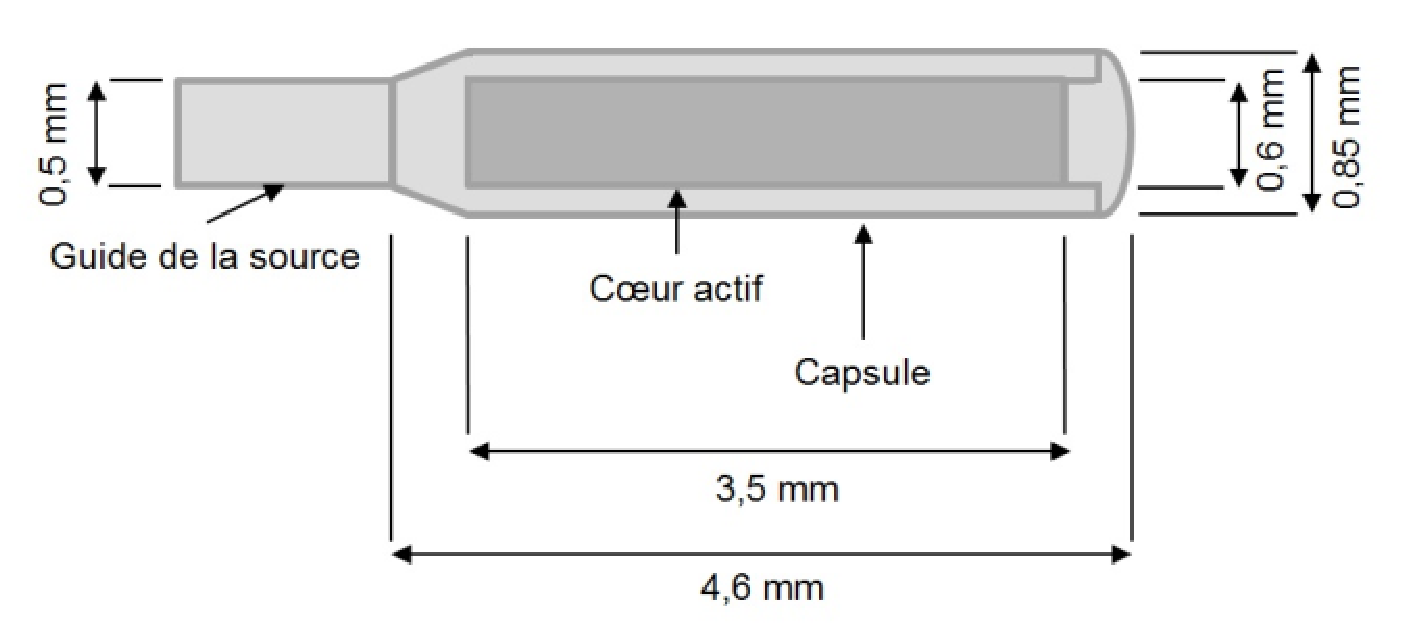
\includegraphics[width=11.0cm,height=5.0cm]{Flexitron.eps}
\caption{\label{Flexitron} Schéma de la composition de la source d’Iridium-192 se trouvant dans le Flexitron de la compagnie Elekta (Alizadeh et al., 2015).}
\end{figure}
%
\section{Équipement de traiment}
La forme de la curiethérapie sur laquelle repose le présent projet est la curiethérapie haut débit de dose (HDD) pour le cancer de la prostate. Les équipements nécessaires pour délivrer ce type de traitement sont un gabarit qui guide l’implantation des cathéters dans la prostate (figure \ref{GabaritProstate}). Le geste du radio-oncologue dans l’implantation des cathéters est guidé par une échographie transrectale (figure \ref{ImagerieSonde}). Lorsque tous les cathéters sont implantés, le patient passé au scanner pour l’acquisition des images pour la dosimétrie et par la suite, un projecteur de source contenant une source d’Iridium-192 est utilisé pour la délivrance de la dose (figure \ref{ProjecteurSource}).
%
\begin{figure}[http]
\centering
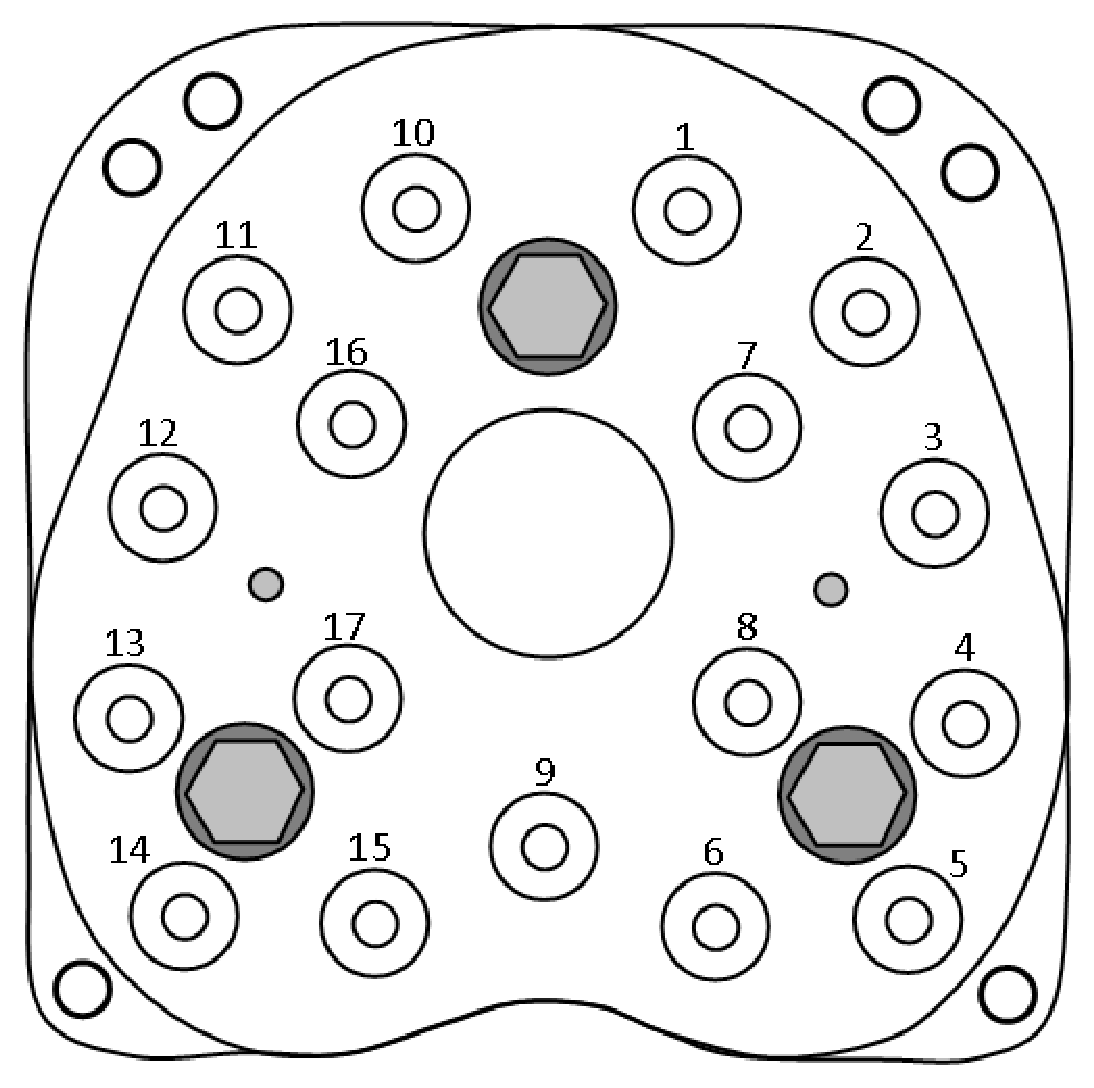
\includegraphics[width=5.5cm,height=5.3cm]{GabaritProstate.eps}
\caption{\label{GabaritProstate} Gabarit de Nucletron utilisé en curiethérapie de la prostate pour l’implantation des cathéters.}
\end{figure}
%
Les différents équipements cités ci-dessus appartiennent à une chaîne globale de traitement en curiethérapie HDD, qui s’étend de la phase diagnostique jusqu’à la délivrance de la dose. Lors de l’acquisition de ces équipements, leurs normes de fonctionnement qui avaient été considérées comme étant acceptables par le biais d’une phase de commissionnement, doivent être maintenues tout le long de leur durée d’exploitation, d’où l’intérêt d’un programme de contrôle qualité (CQ). \nomenclature{QC}{Contrôle Qualité} Ce programme de CQ s’insère dans d’un cadre plus global d’un programme d’assurance qualité de l’Hôpital. La section qui suit décrit les grandes lignes d’un programme de CQ en curiethérapie HDD et la phase de ce programme dans laquelle s’inscrit ce projet.
%
\begin{figure}[!ht]
\centering
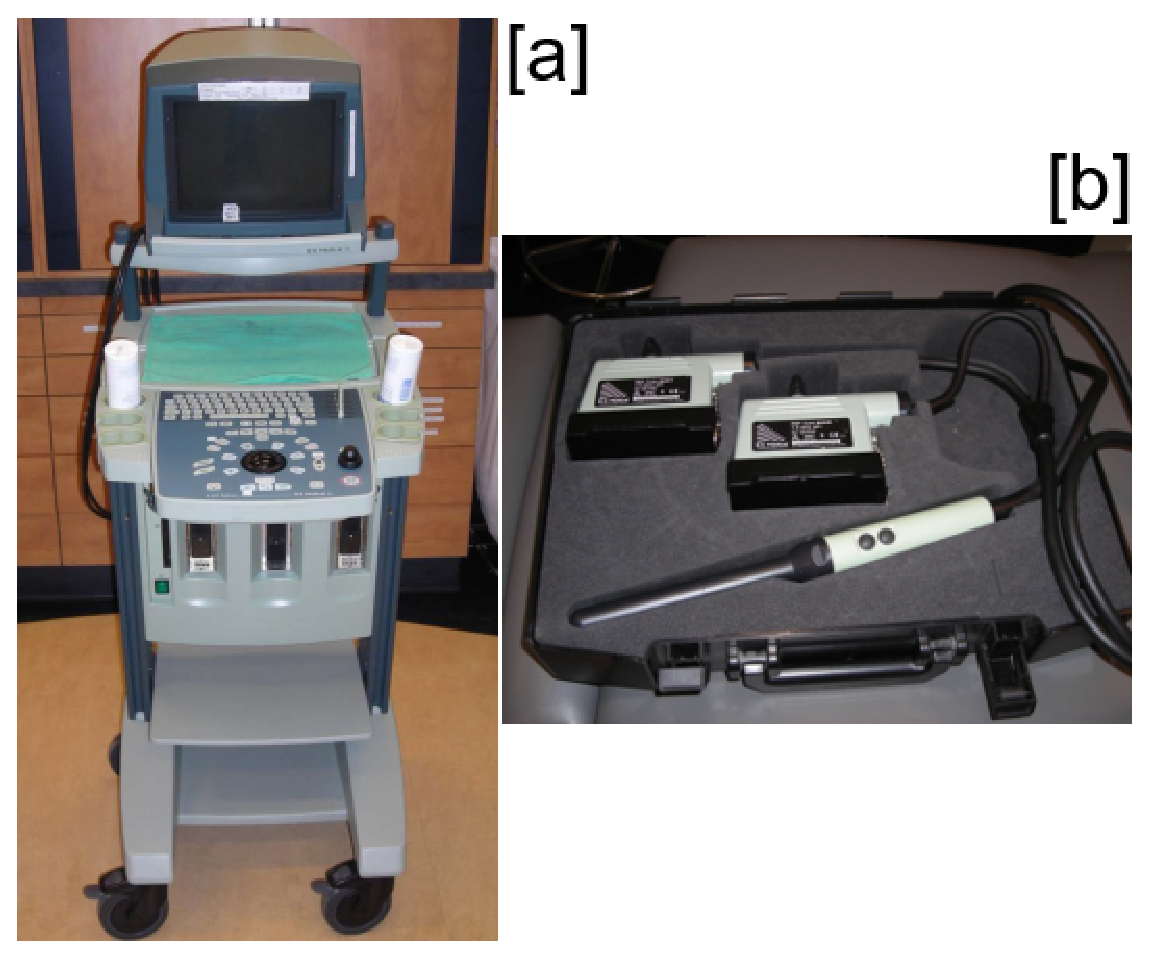
\includegraphics[width=8.5cm,height=6.5cm]{ImagerieSonde.eps}
\caption{\label{ImagerieSonde} Système d’échographie pour la localisation de la prostate et le guidage d’implantation des cathéters. Console d’acquisition et de visualisation (a) et sonde transrectale (b).}
\end{figure}
%
\begin{figure}[!ht]
\centering
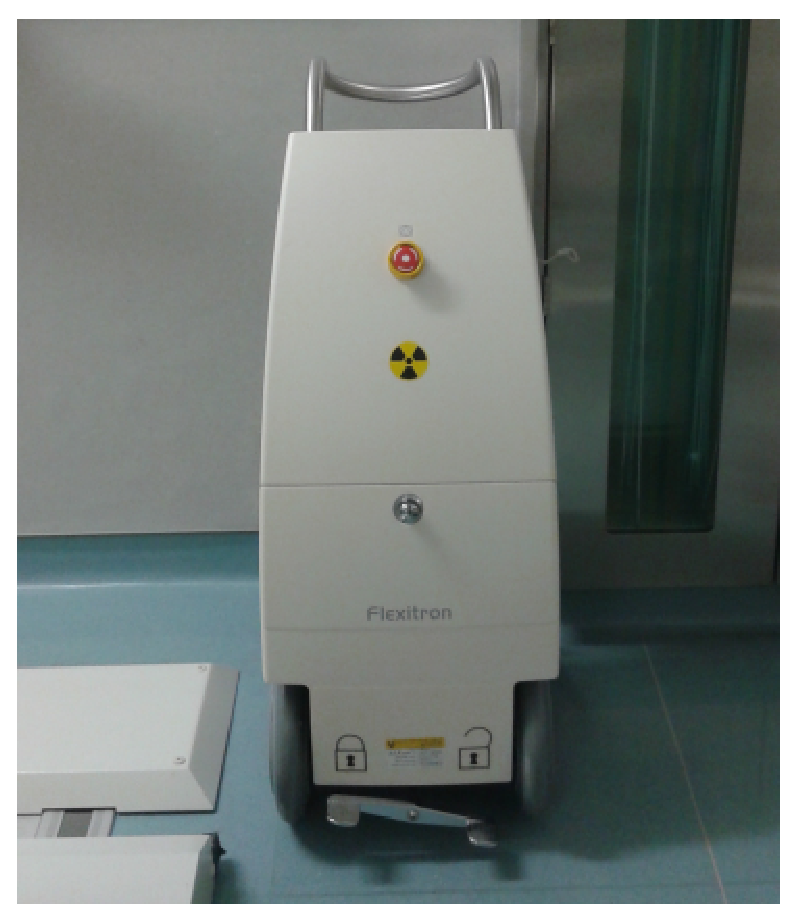
\includegraphics[width=6.0cm,height=7.0cm]{ProjecteurSource.eps}
\caption{\label{ProjecteurSource} Projecteur de source de marque Flexitron de la compagnie Elekta contenant une source d’Iridium-192.}
\end{figure}
%
\vspace{3cm}
\section{Assurance qualité et contrôle qualité en curiethérapie HDD}
\subsection{Assurance qualité}
L’assurance qualité (AQ) \nomenclature{AQ}{Assurance Qualité} et le CQ sont deux aspects importants en radiothérapie qui permettent de garantir la fiabilité et la précision de la dose délivrée au patient. Un programme d’AQ bien établi réduit les incertitudes et les erreurs dans la dosimétrie, la planification du traitement, la performance des équipements, la délivrance de la dose et, par conséquent, garantit la réalisation des objectifs cliniques.
%
\begin{itemize}[label=\textbullet, font=\LARGE]
	\item \textbf{Définition générale}\newline
	L'assurance qualité est l'ensemble des actions planifiées et systématiques nécessaires pour assurer avec une confiance 			suffisante qu'un produit ou un service satisfait aux exigences de qualité \cite{Podgorsak}.
    %
	\item \textbf{AQ en radiothérapie} \newline
	Dans le contexte de la radiothérapie, l’AQ est l’ensemble des procédures qui garantissent la cohérence d’une prescription 		médicale et l’exécution sécuritaire de celle-ci afin de délivrer la dose prescrite au volume cible, tout en minimisant la dose 		aux tissus normaux alentour, l’exposition du personnel et en garantissant la surveillance convenable du patient en vue 			d’évaluer le résultat final du traitement. Une telle définition englobe plusieurs aspects sur le plan organisationnel 			concernant, notamment, la prise en charge et le suivi adéquat des patients, la répartition des responsabilités, la formation et 	la gestion des équipements \cite{Podgorsak, Lisbona}.
\end{itemize}
% 
\subsection{Contrôle qualité}
Le  CQ est un des éléments essentiels d’un programme d’AQ si l’on veut garantir un niveau de confiance élevé dans l’utilisation des équipements, ou des procédés qui interviennent dans la chaîne de traitement. Il s’agit donc d’un processus réglementaire par lequel les performances réelles de la qualité sont mesurées par rapport aux normes existantes, et les mesures nécessaires sont prises pour maintenir, ajuster, ou corriger ces performances si les écarts de conformité aux normes sont observés.\newline 
En curiethérapie HDD, le contrôle qualité concerne:
%
\begin{itemize}[label=\textbullet, font=\LARGE]
\item Les équipements d'imagerie qui sont à la base du diagnostic, et qui fournissent des informations utiles pour la planification du trainement, à savoir, Le scanner, l’imagerie par résonance magnétique (IRM), \nomenclature{IRM}{Imagerie par Résonance Magnétique} la tomographie d’émission monophotonique couplée au scanner (SPECT/CT), \nomenclature{SPECT}{Single-Photon Emission Computed Tomography} la tomographie par émission de positons couplée au scanner (PET/CT) \nomenclature{PET}{Positron Emission Tomography} et l’échographie (CT). \nomenclature{CT}{Computed Tomography (Scanner)}
%
\item Les projecteurs de sources qui permettent de délivrer la dose au patient en assurant la radioprotection de ce dernier et celle du personnel.
%
\item les systèmes de planification de traitement (TPS) et les algorithmes de calcul de dose qui leur sont associés.
\end{itemize}
%
Le présent projet dont un des aspects est l’introduction d’un nouveau concept du CQ, s’insère dans la phase de la planification du traitement en curiethérapie HDD pour le cancer de la prostate.
%
\section{Le cancer de la prostate}     % numéroté
\subsection{Incidence et mortalité}
Le cancer est classé par l’Organisation Mondiale de la Santé (OMS) \cite{OMS} \nomenclature{OMS}{Organisation Mondiale de la Santé} comme étant la deuxième cause de mortalité dans le monde. Les dernières statistiques de GLOBOCAN 2012 \cite{GLOBOCAN} publiées en décembre 2013 estiment à 14,1 millions, le nombre de nouveaux cas de cancer et à 8,2 millions le nombre de décès liés au cancer survenus en 2012, en comparaison respectivement à 12,7 et 7,6 millions en 2008. L’OMS souligne qu’en 2015, 8,8 millions de décès sont attribués au cancer et que, près d’un décès sur 6 dans le monde est dû au cancer. Ces chiffres interpelant peuvent s’expliquer par plusieurs facteurs, entre autres : la croissance démographique et le vieillissement de la population, une augmentation de la prévalence des facteurs de risques bien établis tels que le tabagisme, le surpoids et l’inactivité physique \cite{Torre}. Sur le plan national, la publication \enquote{statistique canadienne sur le cancer} diffusée le 20 juin 2017 \cite{StatCanada} indique que le cancer est la première cause de mortalité au Canada, soit \textasciitilde 30\% par rapport aux autres maladies. La figure \ref{FigureStatCancer1} \cite{StatCanada} illustre le taux de mortalité au Canada en 2012, pour l’ensemble des causes de décès confondus.
%
\begin{figure}[ht]
\centering
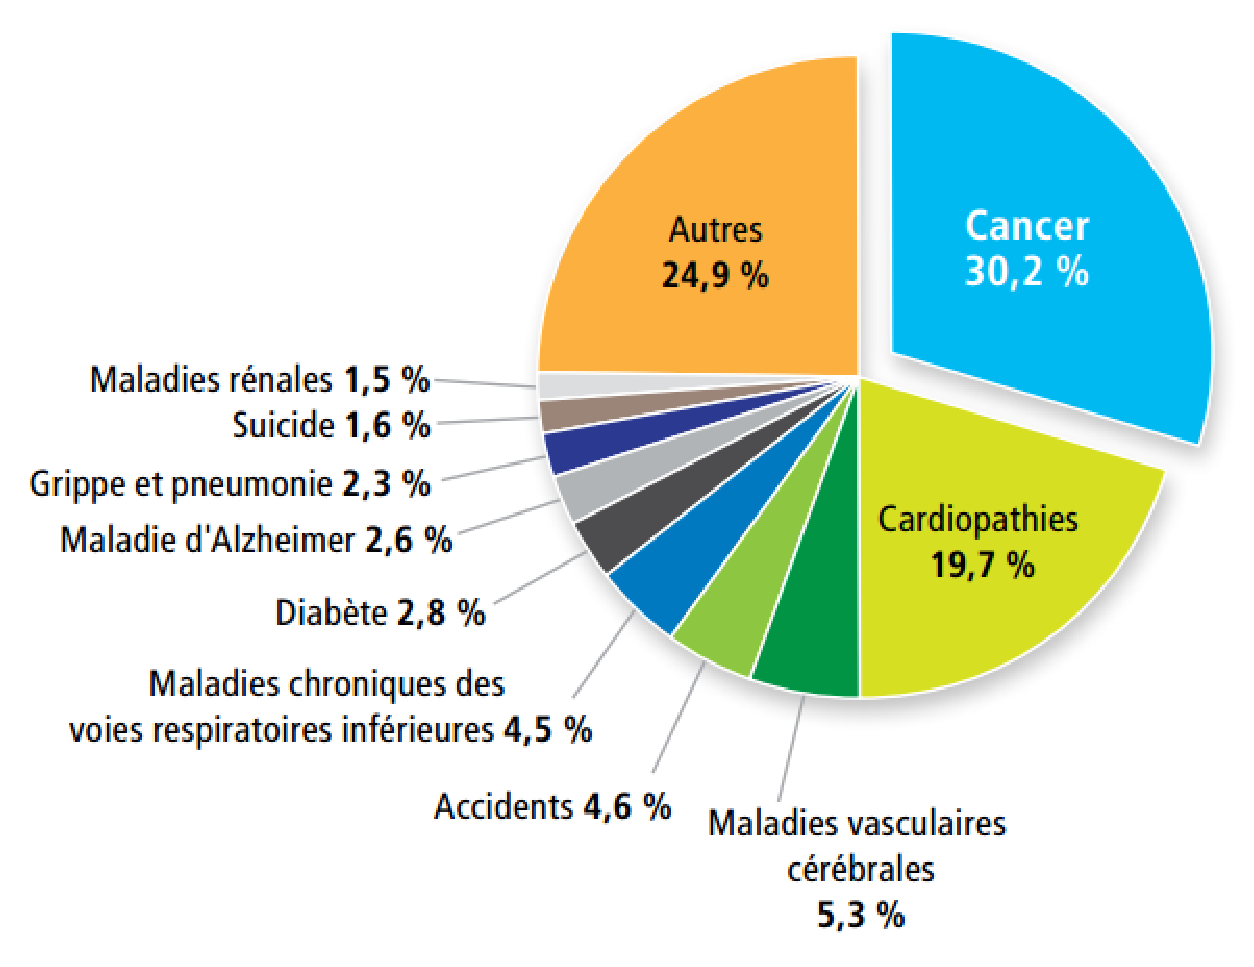
\includegraphics[width=7.3cm,height=5.5cm]{FigureStatCancer1.eps}
\caption{\label{FigureStatCancer1} Taux de mortalité au Canada en 2012, toutes causes confondues.}
\end{figure}
%
Les estimations sur l’incidence (respectivement pour la mortalité) pour les hommes en 2017 sont \textasciitilde 100 000 (respectivement 42 600) nouveaux cas. La projection de nouveaux cas en 2017 pour le cancer de la prostate est 20,7\%, suivi du cancer colorectal (14.5\%) et le cancer des poumons et bronches (14\%). Les chiffres sans doute alarmants présentés ci-dessus, aussi bien sur le plan mondial que national, peuvent expliquer la grande mobilisation observée dans le monde pour la recherche sur le cancer; recherches orientées soit dans le perfectionnement des méthodes de traitements actuellement utilisées en clinique, ou dans le développement de nouvelles possibilités thérapeutiques.
%
\subsection{Anatomie et physiologie}
La prostate fait partie du système génital masculin. Chez les jeunes hommes, elle a la taille d’une noix qui augmente progressivement de volume à la fin de la quarante et début de la cinquante. Elle joue un rôle important pour la fertilité de l’homme, notamment, en participant à la formation et la maturation des spermatozoïdes. Sa localisation lui confère également un rôle dans le bon fonctionnement de l’appareil mictionnel étant donné qu’elle est étroitement liée aux deux sphincters qui assurent une bonne continence urinaire. Comme le montre la figure \ref{FigureProstate} \cite{ImageProstate}, la position de la glande prostatique est dans le petit bassin. Sur sa partie supérieure appelée base, repose la partie inférieure de la vessie. Elle est localisée en arrière du pubis et devant le rectum. Les organes à risques primordiaux qui compromettent la dosimétrie pour le cancer de la prostate sont la vessie, le rectum et l’urètre dont une partie est contenue dans la prostate (urètre prostatique).
%
\begin{figure}[ht]
\centering
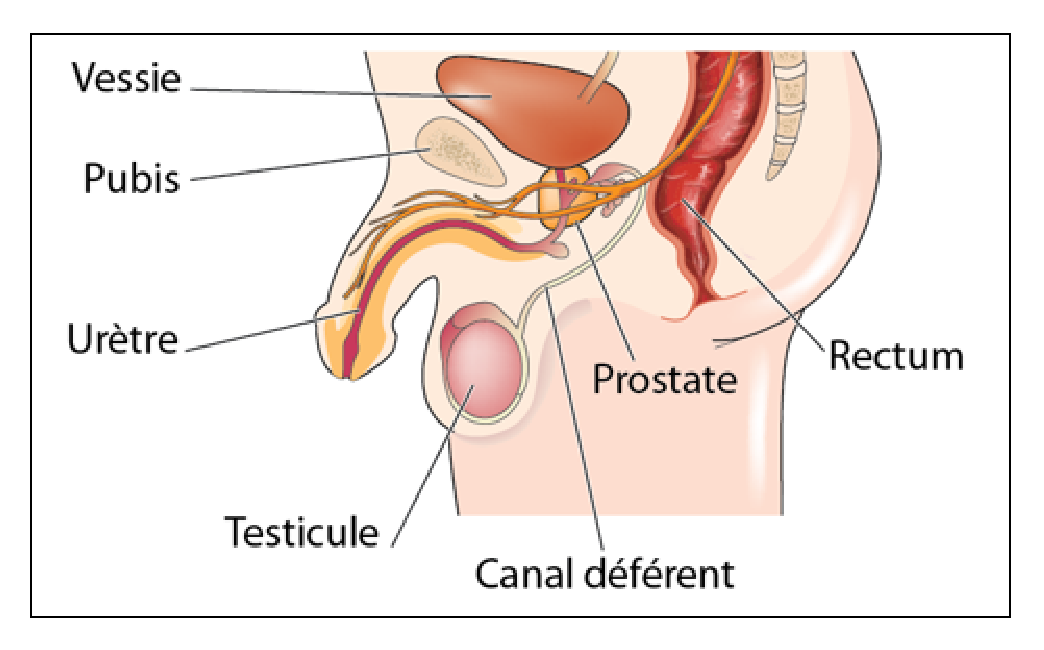
\includegraphics[width=8.5cm,height=6.5cm]{FigureProstate.eps}
\caption{\label{FigureProstate} Anatomie de la prostate et sa localisation par rapport à la vessie et le rectum.}
\end{figure}
%
\subsection{Diagnostique}
L’approche standard pour le diagnostic du cancer de la prostate repose sur la combinaison des résultats d’un test d’antigène prostatique spécifique (APS) \nomenclature{APS}{Antigène Prostatique Spécifique}, le toucher rectal (TR) \nomenclature{TR}{Toucher Rectal} permettant de vérifier la taille et la forme de la prostate, une échographie transrectale (ETR) \nomenclature{ETR}{Échographie Transrectale} ou une biopsie. Il existe une certaine complémentarité entre les différents examens cités ci-dessus; par exemple, le médecin peut faire recours à une ETR pour le diagnostic du cancer de la prostate si l’APS est élevé ou si une région anormale a été détectée lors du TR.   La connaissance du stade du cancer est un élément clé dans cette phase de dépistage, puisque celle-ci détermine le choix de la modalité de traitement, ainsi que le pronostic sur la survie du patient. Cette stadification clinique est effectuée par les médecins en s’appuyant sur le système international TNM \cite{Sobin} dans lequel, \enquote{T} désigne le type de la tumeur, \enquote{N} la présence de la tumeur dans les ganglions lymphatiques et \enquote{M} la présence de la tumeur dans d’autres régions éloignées (métastases). Le tableau \ref{StadificationProsatate} ci-dessous résume cette stadification clinique pour les différents types de tumeurs et les détails de la classification N et M relatifs à leur caractère envahissant peuvent être consultés dans les travaux de Sobin et al.\cite{Sobin}. La stadification TNM est toujours associée au score de Gleason \cite{Chen, Salomon} créé dans les années 1960-1970 et redéfini en 2005, score qui fait référence au degré d’agressivité du cancer de la prostate.
%
\begin {table}[ht]
%\begin {center}
\caption{Stadification clinique du cancer de la prostate en fonction du type de la tumeur.}
\label{StadificationProsatate} 
\renewcommand{\arraystretch}{1.4}
	\begin{tabular}{p{5.5cm} p{9.0cm}}
		\toprule[1.3pt]
        \hline
        Stadification clinique                   &      Description   \\ 
        \hline
        T1               			   & Ce stade concerne les tumeurs de petites tailles se limitant à la prostate, invisibles à l'imagerie et pour lesquelles, il est impossible de palper par le biais du toucher rectal. Il s’agit d’un stade qui ne produit généralement aucun symptôme.                                  \\ 
        T2               			   & La tumeur est détectable par le toucher rectal, mais limitée à la prostate.                               \\ 
        T3               			   & Ce stade concerne les tumeurs pour lesquelles les cellules cancéreuses se sont propagées au-delà de la prostate, mais localisables dans les régions qui entourent la glande.                                \\
        T4               			   & Tumeurs pour lesquelles les cellules cancéreuses se sont propagées au-delà de la prostate dans les structures avoisinantes (sphincter externe, rectum, muscles releveurs de l’anus ou paroi pelvienne).                                \\ 
        M               			   & Il s’agit d’un stade pour lequel la tumeur s’est propagée dans les régions éloignées (métastase), au-delà de la prostate (os, foie, poumons) par l’intermédiaire du système lymphatique et/ou par la circulation sanguine.                                 \\ 
        \bottomrule[1.3pt]
	\end{tabular} 
	%\end {center}
\end {table}
%
\subsection{Place de l'imagerie pour la curiethérapie de la prostate HDD}
Ces dix dernières années ont été marquées par des avancées technologiques qui ont rendu possible l’utilisation de l’imagerie prostatique dans le processus de détection, localisation et stadification du cancer de la prostate, en complément de l’APS, le TR, l’ETR ou la biopsie. Les principales modalités d’imagerie telles que le scanner, l’échographie, l’IRM et le PET sont actuellement utilisées pour la localisation des cellules cancéreuses et la détermination de leur extension dans les structures éloignées de la prostate (métastases), la stadification, le guidage en temps réel de l’implantation des cathéters dans la glande, ainsi que la surveillance active du patient. Les paragraphes suivants sont consacrés à la description succincte de quelques-unes de ses techniques, ainsi que leurs principales utilisations.
%
\subsection*{\textbf{Échographie prostatique}}
L’échographie est la technique d’imagerie la plus ancienne et reste largement parmi les techniques les plus utilisées dans le processus de prise en charge du cancer de la prostate. Les indications de cette technique sont, entre autres, le guidage en temps réel du prélèvement des échantillons de tissus prostatiques pour la biopsie et l’implantation des cathéters dans la prostate, une délinéation claire de la prostate ainsi que la détermination de son volume \cite{Sarkar, Taneja, Dubinsky, Kirkham, Holm2002}. Le principe physique de la technique repose sur la mesure des ondes mécaniques de compression se propageant dans un milieu tissulaire. La propagation de ces ondes à l’interface de deux tissus ayant des propriétés acoustiques différentes obéit aux lois analogues à celles de l’optique ondulatoire (réflexion, réfraction, diffusion et absorption). Le signal qui résulte de la partie réfléchie de l’onde est recueilli par un transducteur (émetteur et récepteur d’impulsions ultrasonores), traité et synthétisé en ton de gris des tissus pour produire une image statique ou dynamique. L’impédance acoustique qui est une caractéristique propre à chaque tissu, et responsable de l’imagerie échographique est donnée par l’équation \eqref{eqn:imp} dans laquelle, $\rho \left(kg/m^{3}\right)$ est la densité des tissus et $c \left(m/s\right)$ la vitesse du son  qui varie en fonction du type de tissu dans lequel la propagation a lieu.
%
\begin{equation}\label{eqn:imp}
	z = \rho \times c
\end{equation}
%
Les différences de densité et de vitesse de propagation à l’interface des tissus sont donc des propriétés fondamentales pour la génération des échos et le contraste dans le processus de formation de l’image échographique. Cependant, les systèmes médicaux approximent généralement la vitesse des ondes dans les milieux biologiques à celle des tissus mous, soit 1540 m/s \cite{Bushberg}, seule la densité est donc prise en compte pour la différenciation des différents tissus. Les coefficients de transmission (T) et réflexion (R) d’une onde acoustique arrivant normalement à l’interface de deux tissus d’impédances acoustiques z$_{1}$ et z$_{2}$ sont donnés par l’équation \eqref{eqn:reflex_Trans},
%
\begin{equation}\label{eqn:reflex_Trans}
	T = \frac{4z_{1}z_{2}}{\left(z_{1}+z_{2}\right)^{2}}, \qquad R = 1-T
\end{equation}
%
L’équation \eqref{eqn:reflex_Trans} explique la nécessité de l’utilisation d’un gel entre le transducteur et la peau, aux interfaces muscle-air; la transmission étant \textasciitilde 100\% en l’absence du gel \cite{ EPoulin}. L’inconvénient majeur de l’échographie est son contraste tissulaire limité entre le tissu cancéreux et bénin, limitation qui est grandement améliorée par l’imagerie par résonance magnétique.
%
\subsection*{\textbf{Imagerie par résonance magnétique}}
L’imagerie par résonance magnétique (IRM) présente un avantage de produire des images anatomiques avec une résolution en contraste relativement élevée, ce qui permet un meilleur diagnostic du cancer de la prostate. L’IRM anatomique (pondération T$_{2}$) est généralement associée à l’IMR fonctionnelle (séquences de perfusion et de diffusion) pour les examens cliniques de routine \cite{Horwitz}. Une telle combinaison qui est connue sous le nom de l’IMR multiparamétrique, conduit à des résultats plus fiables que les images pondérées T$_{2}$ seulement pour le diagnostic initial, le bilan d’extension métastatique, la présence de grade de Gleason élevé et la surveillance active du patient. Le principe physique de l’IRM repose sur les propriétés magnétiques de la matière. En effet, le corps humain est constitué en grande partie (environ 70\%-80\% du poids du corps) par les molécules d’eau (H$_{2}$O). Les noyaux d’atomes d’hydrogène sont constitués d’un proton qui, du point de vue magnétique, sont assimilables à des petits moments magnétiques de spin ($\mu$). En l’absence d’un champ magnétique externe, l’orientation de ces moments magnétiques est aléatoire dans la matière, ce qui conduit à une aimantation macroscopique (M) nulle. L’application d’un champ magnétique externe B$_{0}$ fait tourner les moments magnétiques de spin autour de la direction de B$_{0}$ et chaque moment décrit un cône de révolution autour de cette direction, ce qui fait apparaître une aimantation longitudinale M$_{z}$ et transversale M$_{xy}$. En présence de du champ B$_{0}$, le processus d’acquisition de l’image passe d’abord par une phase d’excitation par une onde radiofréquence (RF) à la fréquence dite de Larmor ($\nu_{0}$, fréquence de résonance du système) donnée par l’équation \eqref{eqn:FLarmor1} dans laquelle $\gamma$ représente le rapport gyromagnétique.
%
\begin{equation}\label{eqn:FLarmor1}
	\nu_{0}= \frac{\gamma}{2\pi}B_{0}
\end{equation}
%
Cette excitation va créer une situation de déséquilibre dans laquelle, l’aimantation longitudinale va décroitre et la composante transversale va croitre. L’intensité et la durée de l’impulsion RF déterminent l’angle de basculement. À la fin de l’impulsion RF, l’aimantation revient à sa position d’équilibre (phénomène de relaxation) tout en émettant un signal (courant induit dû à la décroissance exponentielle de M$_{xy}$) qui est recueilli par des antennes réceptrices. Le retour à l’équilibre se fait pendant un intervalle de temps T$_{2}$ pour l’aimantation transversale et T$_{1}$ pour l’aimantation longitudinale. T$_{2}$ est caractéristique de chaque tissu, ce qui permet de différentier les différents tissus excités. Cependant, le signal recueilli provient de tout l’échantillon, d’où la nécessité d’une technique de codage par application d’un gradient de champ magnétique dans la même direction que B$_{0}$ (gradient de sélection de coupe G$_{z}$) donnée par la relation :
%
\begin{equation}\label{eqn:Gradient}
	B(z)= B_{0}+G_{z}z
\end{equation}
%
La fréquence de résonance du système prend donc la forme de l’équation \eqref{eqn:FLarmor2}, ce qui permet de sélectionner le volume anatomique à explorer et d’analyser que le signal provenant de ce dernier.
%
\begin{equation}\label{eqn:FLarmor2}
	\nu_{z}= \frac{\gamma}{2\pi}B(z)
\end{equation}
%
La position de chaque point dans le volume anatomique excitée est par la suite encodée par application d’un grandirent de codage en phase et en fréquence dans l’espace de fourrier. Ce codage spatial en fréquence et en phase permet par la suite, moyennant une transformation de Fourier du signal, de reconstruire l’image de la coupe. Les détails complémentaires sur le principe physique de l’IRM peuvent être consultés dans la littérature \cite{Bushberg, Grover, HENDEE}. Les deux inconvénients majeurs de l’IRM sont la nature statique des images reconstruites et le coût d’acquisition de la technologie élevée.
%
\subsection*{\textbf{Scanner abdomino-pelvien}}
Les images CT continuent à avoir leur place dans le processus de prise en charge du cancer de la prostate. Dans la phase diagnostique, ils permettent la recherche de métastases ganglionnaires chez les patients à risque élevé ou intermédiaire. Ces images sont également déterminantes lors de la phase de planification, notamment pour la reconstruction des cathéters et le calcul prévisionnel de la dose. Le principe physique de cette technique repose sur l’atténuation des photons émis par un tube à rayons X. En effet, lors de la traversée d’un faisceau de rayons X dans un milieu d’épaisseur $x$, les photons subissent plusieurs types d’interactions physiques avec les atomes du milieu, conduisant à leur absorption ou leur diffusion. Si l’on désigne par I$_{0}$ l’intensité du faisceau à l’entrée du milieu, l’intensité de ce dernier à la sortie après un parcours d’épaisseur $x (cm)$ est régit par une loi d’atténuation exponentielle donnée par l’équation \eqref{eqn:APhotons},
%
\begin{equation}\label{eqn:APhotons}
	I(x)= I_{0} exp\left(-\mu x\right)
\end{equation}
%
$\mu (cm^{-1})$ est le coefficient d’atténuation linéaire qui dépend du numéro atomique du milieu, sa densité et l’énergie du rayonnement incident. Techniquement, le scanner est une chaîne radiologique constituée d'un tube à rayons X et un ensemble de détecteurs disposés en couronne. Au cours de l’acquisition, l’ensemble tube-détecteurs tourne autour du patient pendant que la table avance en continu à vitesse constante (acquisition hélicoïdale), ou avance après l’acquisition des données d’une coupe (acquisition séquentielle). Les détecteurs transforment l’énergie radiante des photons X en signal électrique dont l’amplitude est proportionnelle à l’intensité du faisceau incident. Un profil d’atténuation regroupe la totalité des signaux électriques générés par tous les détecteurs pour un angle de rotation donné. Plusieurs profils d’atténuation à différents angles de rotation sont enregistrés, échantillonnés et numérisés. Ces données sont ensuite rétro-projetées dans une matrice de reconstruction, puis transformées en image.  En effet, la matrice de données est composée de n lignes et  n colonnes, chaque élément de cette matrice est un pixel contenant une valeur d’atténuation ou de densité dans l’échelle des gris. Les coefficients d’atténuation des différents tissus sont normalisés à celui de l’eau et exprimés en unités Hounsfield (UH), en l’honneur de Sir Godfrey Hounsfield qui a été l’un des principaux innovateurs de la technologie CT, selon l’équation \eqref{eqn:Hounsfield},
%
\begin{equation}\label{eqn:Hounsfield}
	UH\left(x, y, z\right)= 1000 \left[\frac{\mu\left(x,y,z\right)-\mu_{eau}}{\mu_{eau}}\right]
\end{equation}
% 
$\mu\left(x,y,z\right)$ est la valeur moyenne du coefficient d’atténuation linéaire pour un élément de volume (voxel) du tissu dans le patient, à la position $(x, y, z)$ et $\mu_{eau}$ le coefficient d'atténuation linéaire de l'eau pour le spectre des rayons X utilisé. Une telle normalisation conduit à UH$_{eau}=0$, -1000 (air), 280 à 230 (tissus adipeux).
%
\section{Planification du traitement en radiothérapie}
De façon générale, les TPS sont utilisés en radiothérapie pour générer la balistique du traitement permettant d’obtenir une distribution de dose prescrite et uniforme dans le volume cible, tout en minimisant l’irradiation des tissus sains alentour \cite{Thomadsen1, Venselaar, Gerbaule}. La prise en charge d’un patient pour un traitement en radiothérapie est subdivisée en plusieurs étapes, la première étant la phase du diagnostic (acquisition d’images diagnostiques, stadification de la tumeur, bilan d’extension, score de Gleason, etc.). Cette première phase va conduire à la décision de traiter et au choix de la modalité de traitement si le diagnostic est positif. La deuxième phase consiste en l’acquisition des images permettant le contourage du volume cible et les OARs environnants à l’aide des modalités d’imagerie telles: le CT, l’IRM, l’échographie, etc. Le processus de contourage du volume cible devant recevoir la dose prescrite est guidé par les recommandations de la commission internationale des unités et mesures radiologiques (ICRU) dans ces rapports 50 et 62 \nomenclature{ICRU}{International Commission on Radiation Units and Measurements} \cite{ICRU50, ICRU62}. Ces recommandations définissent un vocabulaire cohérent sur la définition des volumes cibles, reconnu et compris au niveau de chaque institution, et au niveau international. Les principaux volumes définis dans ces recommandations sont :
%
\begin{itemize}[label=\textbullet, font=\LARGE]
\item \textbf{Volume tumoral macroscopique (GTV)} : \nomenclature{GTV}{Gross Tumour Volume} \newline
Il est constitué par l’ensemble des lésions tumorales, mesurables, palpables ou visibles avec une des modalités d’imagerie actuelle. 
%
\item \textbf{Volume cible anatomoclinique (CTV)}: \nomenclature{CTV}{Clinical Target Volume}\newline
Il comprend le volume anatomique dans lequel on veut éradiquer la maladie (GTV) et les extensions microscopiques des cellules cancéreuses qui peuvent être considérées avec une certaine probabilité comme pertinentes pour le traitement. Il s’agit d’une expansion géométrique autour du GTV pour tenir compte des incertitudes anatomocliniques.
%
\item \textbf{Volume cible prévisionnel (PTV)}: \nomenclature{PTV}{Planning Target Volume }\newline
Il s’agit d’un concept géométrique introduit pour les besoins de la planification et de l’évaluation. Il est défini pour assurer avec une probabilité cliniquement acceptable que la dose prescrite est délivrée dans le CTV. Ce volume vise à tenir compte des variations de la position du CTV, de sa forme et de ses dimensions; variations dues aux mouvements du patient ou de ses organes (respiration, battements cardiaques, remplissage de la vessie ou du rectum, déglutition). Il tient également compte des incertitudes liées à l'imperfection de la balistique du traitement.
%
\end{itemize}
%
Cette phase de courage des volumes d’intérêt est suivie du calcul prévisionnel de la distribution de dose qui sera délivrée au patient avec un TPS. Il s’agit de la phase durant laquelle toute la balistique du traitement est mise en place.\newline
Dans le cas particulier de la planification du cancer de la prostate en curiethérapie HDD, l’ordre des étapes décrites ci-dessus est quelque peu modifié. Après la phase diagnostique conduisant à la décision de traiter en curiethérapie HDD, le radio-oncologue procède à la mise en place des cathéters dans la glande prostatique à l’aide d’un gabarit sous guidage échographique. L'implantation des cathéters se fait au bloc opératoire, sous anesthésie générale. Par la suite, une série d’images est prise au CT, ces images visent deux objectifs principaux :
%
\begin{itemize}[label=\textbullet, font=\LARGE]
	\item Permettre le contourage de toutes structures anatomiques d'intérêt, notamment, la prostate, l'urètre, la vessie et le 	rectum.
    %
	\item Permettre la reconstruction des cathéters. En effet, les cathéters sont distinguables des tissus biologiques, car ils 	sont faits d’un matériau CT compatible pour la réduction des artéfacts métalliques et ils contiennent de l’air.
    %
\end{itemize}
%
Contrairement à la radiothérapie externe, la planification avec le TPS en curiethérapie HDD consistera à déterminer les positions de la source radioactive dans chaque cathéter (dwell positions) et le temps d’arrêt de la source à chacune des positions (dwell time). En planification inverse, les objectifs cliniques du traitement, c’est-à-dire, la couverture du CTV et la limitation de la dose aux OARs sont introduits dans le TPS et servent de point de départ pour trouver le plan optimal (meilleure combinaison dwell position et dwell time). Il s’agit d’un processus itératif au cours duquel, l’algorithme de calcul implanté dans le TPS explore l'espace des solutions (plans de traitement réalisables) et le planificateur adopte le plan qui satisfait le mieux les objectifs cliniques. Les sections \ref{sssec:TG-43} et \ref{sssec:optimis} qui suivent sont consacrées à la présentation du formalisme TG-43 et une brève description de quelques algorithmes d’optimisation implantés dans les TPS.
%
\subsection{Formalisme du calcul de dose: AAPM TG-43}\label{sssec:TG-43} 
\nomenclature{AAPM}{American Association of Physicists in Medicine}
En 1995, le groupe de travail N$^{o} 43$ \cite{AAPMTG-43} de l'American Association of Physicists in Medicine (AAPM) a publié un rapport sur la dosimétrie des sources utilisées en curiethérapie interstitielle. Ce rapport, suivi de ces mises à jour publiées en 2004 et 2017 \cite{AAPMTG-43R1, AAPMTG-43R2} présentent le formalisme de calcul de dose utilisé dans tous les TPS actuels. Il convient cependant de souligner que le formalisme TG-43 a été initialement développé pour la dosimétrie des sources en curiethérapie bas débit de dose telles que l'${}^{125}$I et le ${}^{103}$Pd, mais ce dernier est largement accepté sur le plan international et utilisé pour la dosimétrie des sources à haute énergie pour la curiethérapie HDD et débit de dose pulsé \cite{Venselaar}. Ces recommandations introduisent de nouvelles quantités physiques telles que : le débit de kerma de référence ($S_{k}$), la constante de débit de dose ($\Lambda$), la fonction de dose radiale ($g(r)$), la fonction d’anisotropie ($F(r, \theta)$) et la fonction géométrique ($G(r, \theta)$). Le formalisme permet de calculer la distribution de dose en tous points d’un plan passant par l’axe longitudinal de la source, le milieu étant considéré comme infini, homogène et constitué d’eau. La figure \ref{FigureTG-43} montre le système de coordonnées utilisé pour le calcul de la dose en tout point $P(r, \theta)$.
%
\begin{figure}%[h]
\centering
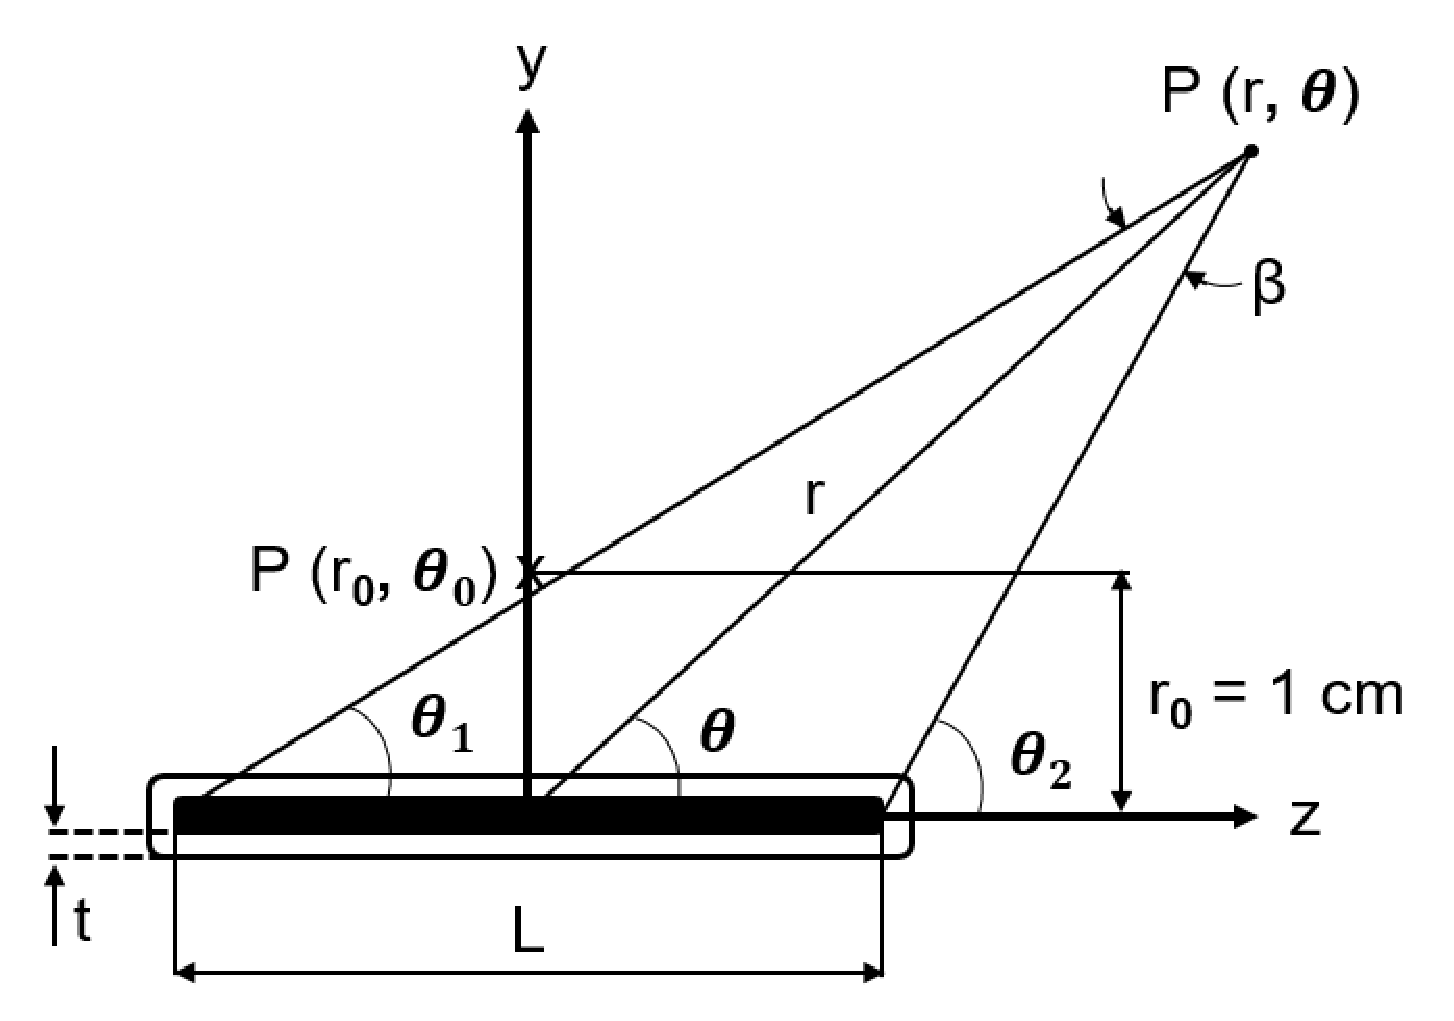
\includegraphics[width=8.0cm, height=6.0cm]{FigureTG-43.eps}
\caption{\label{FigureTG-43} Système de cordonnées utilisé pour le calcul de dose dans le formalisme TG-43 (Nath et al., 1995).}
\end{figure}
%
Le débit de dose $\stackrel{.}{D} (r, \theta)$ dans l’approximation d’une source linéaire est donné par l’équation générale,
%
\begin{equation}\label{eqn:DoseRef}
	\stackrel{.}{D}\left(r,\theta\right)=S_{k}.\Lambda . \frac{G_{L}\left(r,\theta\right)}{G_{L}\left(r_{0},\theta_{0}\right)}.g_{L}\left(r\right).F\left(r,\theta\right)
\end{equation}
%
dans laquelle les différents paramètres signifient :
%
\renewcommand{\arraystretch}{1.5}
\begin{longtable}{p{1.5cm} p{13.4cm}}
r & La distance du centre de partie active de la source au point de calcul $P(r, \theta)$. \\
%
$r_{0}$ & La distance de référence, 1 cm dans le plan transverse de la source à l’angle $\theta = 90^{0}$.\\
%
$S_{k}$ & Le débit de kerma de référence dans l’air exprimé en $\mu Gym^{2} h^{-1}$ et généralement mesuré à 1 m du centre de la source dans le plan transverse de celle-ci. Il représente la puissance de la source. \\
%
$\Lambda$ & La constante de débit de dose : $\Lambda (cGy h^{-1} U^{-1})$ avec $U=\mu Gym^{2} h^{-1}$   permet la conversion du débit de kerma dans l'air au débit de dose dans l'eau au point de référence $P(r_{0}, \theta_{0})$.\\
%
$G_{L}(r, \theta)$ & La fonction géométrique : elle permet d’améliorer la précision des calculs due à l’interpolation des valeurs à partir des données tabulées de la constante de débit de dose à des points discrets. Du point de vue physique, cette fonction apporte une correction de l’effet de la loi de l’inverse carré de la distance, au détriment des phénomènes d’atténuation et de diffusion. \\
%
$g_{L}(r)$ & La fonction de dose radiale, elle prend en compte la diminution du débit de dose sur l’axe traverse de la source due uniquement aux phénomènes de diffusion et d’absorption. \\
%
$F(r, \theta)$ & La fonction d’anisotropie : la variation angulaire des phénomènes d'absorption et de la diffusion des photons, aussi bien dans la capsule contenant la source que dans la source elle-même est prise en compte à différentes distances, par la fonction d'anisotropie. \\
%
\end{longtable}
%
\newpage 
La dose totale en chaque point $i$ dans le volume d’intérêt est obtenue en sommant la contribution de la dose provenant de la position $j$ de la source dans tous les cathéters, suivant l’équation :
%
\begin{equation}\label{eqn:DoseTot}
D_{i}=\sum_{j}\stackrel{.}{D}\left(r_{ij}, \theta_{ij}\right)t_{j}
\end{equation}
%
où $t_{j}$ est le temps d’arrêt de la source aux positions $j$. Cette équation ne prend pas en compte la décroissance radioactive au cours de l’irradiation, hypothèse valide si la durée de l’irradiation est assez petite par rapport à la période radioactive de la source. Bien que ce formalise soit implanté dans les TPS actuels, les méthodes d’optimisation varient d’un TPS à un autre, ce qui conduit à des précisions différentes dans le calcul de la distribution de la dose. La section \ref{sssec:optimis} ci-dessous présente quelques méthodes d’optimisation implantées dans les TPS actuels.
%
\subsection{Revue des méthodes d'optimisation}\label{sssec:optimis} 
La phase d’optimisation est un processus au cours duquel on vise à déterminer la meilleure combinaison des dwell positions et dwell times conduisant à une distribution de dose satisfaisant le mieux les objectifs cliniques. Deux méthodes d’optimisation peuvent être utilisées à cet effet : l’optimisation directe (planification conventionnelle) et l’optimisation inverse. En optimisation directe, le planificateur définit manuellement une première combinaison des dwell positions et dwell times, la dose est calculée et évaluée. Une telle approche nécessite très souvent un test de plusieurs combinaisons de paramètres d’optimisation jusqu’à l’obtention d’une distribution de dose qui satisfasse les exigences relatives à la prescription. En optimisation inverse, le point de départ est définit par les objectifs cliniques, c’est-à-dire, la couverture minimale du CTV et les limites de doses aux OARs et l’algorithme d’optimisation se charge de déterminer la meilleure combinaison des dwell positions et dwell times permettant d’attendre les objectifs fixés. L’introduction des objectifs cliniques au TPS conduit à la construction d’une fonction de coût et le planificateur est souvent amené, de façon itérative, à modifier les pénalités de cette fonction pour chaque organe d’intérêt. Le calcul itératif est ensuite laissé à l’ordinateur jusqu’à la satisfaction des objectifs cliniques, ou lorsque la fonction de coût totale aura atteint sa valeur minimale globale. Les trois algorithmes d’optimisation commercialisés par la compagnie Elekta et implantés dans le TPS Oncentra Brachy (Elekta Brachytherapy, Veneedal, The Netherlands) pour la curiethérapie de la prostate à l’HDQ sont brièvement décrits ci-dessous :\newline
%
\begin{itemize}[leftmargin=0pt, label=\textbullet, font=\LARGE]
\item[] \textbf{IPSA} (Inverse Planning by Simulated Annealing) \nomenclature{IPSA}{Inverse Planning by Simulated Annealing}\newline
L’algorithme IPSA est un outil d’optimisation qui repose sur le principe du recuit simulé utilisé en métallurgie pour améliorer la qualité d’un solide. En métallurgie, la méthode consiste à chercher un état d’énergie minimale correspondant à une structure plus stable d’un métal. En partant d’une haute température dans laquelle le métal est dans l’état liquide, on applique un schéma de refroidissement progressif qui permettra au métal de retrouver sa forme solide la plus stable. L’algorithme IPSA a été développé par Etienne Lessard et Jean Pouliot \cite{ELessard, lessard@2001} dans le cadre d’une collaboration scientifique entre le Centre hospitalier universitaire de Québec et l’Université de Californie à San Francisco. Le processus d’optimisation commence d’abord par la traduction mathématiquement des exigences du médecin en objectifs de dose. Ces objectifs sont des valeurs quantitatives qui définissent des plages de dose acceptables pour un organe donné, ainsi que leur importance relative par rapport aux autres critères cliniques. Ils convertissent la dose délivrée D$_{i}$ selon l’équation \eqref{eqn:DoseTot} en tout point $i$ d’un organe donné, en une valeur de pénalité W$_{i}$ par la relation:
%
\begin{equation}\label{eqn:Penalite}
    W_{i} = \begin{cases}
               m_{min}\left(D_{i}-D_{min}\right)               & \qquad si \quad D_{i} < D_{min} \\
               0                                               & \qquad si \quad D_{min} ≤ D_{i} ≤ D_{max} \\	
               m_{max}\left(D_{i}-D_{max}\right) 			   & \qquad si \quad D_{i} > D_{max} 
           \end{cases}
\end{equation}
%
Les différents paramètres de l'équation \eqref{eqn:Penalite} ci-dessus sont illustrés dans la figure \ref{FigurePenalite}. 
%
\begin{figure}[!ht]
\centering
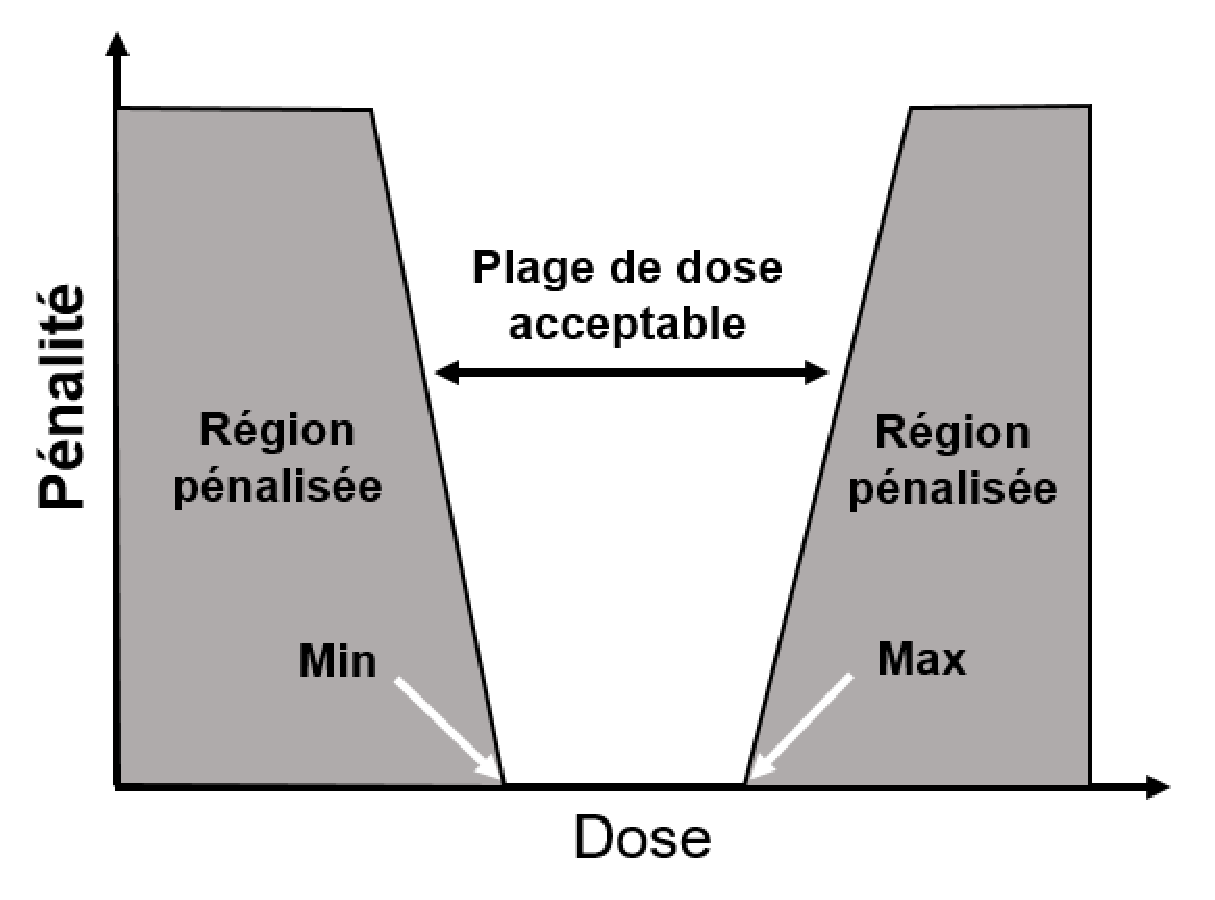
\includegraphics[width=7.5cm, height=6.0cm]{FigurePenalite}
\caption{\label{FigurePenalite} Illustration des différentes régions de dose acceptable et pénalisée.}
\end{figure}
%
D$_{min}$ et D$_{max}$ sont respectivement la valeur minimale et maximale délimitant la plage de dose acceptable. Pour la couverture du CTV par exemple, une dose dans la plage acceptable correspond à une pénalité nulle et à l’extérieure de celle-ci, à une pénalité qui augmente avec un taux égal à m$_{min}$ et m$_{max}$, respectivement pour toute dose D$_{i}$ < D$_{min}$ et D$_{i}$ > D$_{max}$. Le contrôle par le planificateur sur l’ajustement des pentes m$_{min}$ et m$_{max}$ lui permet donc de fixer les importances relatives entre les différents critères cliniques. Plus la pente est élevée, plus la pénalité est forte pour la dose se situant à l’extérieur de la plage acceptable. IPSA permet ainsi de définir deux types de contraintes, à savoir, la contrainte de dose à la surface et dans le volume. Particulièrement pour le CTV, une contrainte de dose à la surface va forcer la conformité de la dose dans son volume, et la contrainte de dose en volume permettra le contrôle de l’homogénéité. On définit une fonction de coût globale qui est la somme de toutes les pénalités W$_{i}$ de la dose en chaque point $i$  pour les contraintes de surface et/ou de volume pour chaque volume d’intérêt (CTV, urètre, vessie, rectum). Cette fonction décrit mathématiquement les objectifs cliniques et est utilisée pour l’évaluation de la distribution de dose; plus cette dernière est proche de la distribution idéale, moins élevée sera la fonction de coût (minimum global).\newline.
%
\item[] \textbf{HIPO} (Hybrid Inverse Planning and Optimization) \nomenclature{HIPO}{Hybrid Inverse Planning and 				Optimization}\newline
Il s’agit d’un algorithme d’optimisation hybride, développé en 2005 pour la planification des traitements en curiethérapie HDD \cite{Karabis}. Le caractère hybride tient du fait que l’algorithme utilise deux méthodes de calcul: (1) le recuit simulé qui est une méthode empirique (métaheuristique) pour optimiser la distribution des cathéters, et (2) une méthode déterministe basée sur le gradient (L-BFGS) \nomenclature{L-BFGS}{Limited-memory Broyden-Fletcher-Goldfarb-Shanno} pour l’optimisation de la distribution de dose. La construction de la fonction coût est basée sur les contraintes de dose en volume et celle-ci pénalise les valeurs de dose qui sont extérieures à la plage de dose acceptable pour chaque structure. Les bornes inférieure ($f_{inf}$) et supérieure ($f_{sup}$) de cette plage de dose sont définies par l’équation \eqref{eqn:FL} pour le CTV et l’équation \eqref{eqn:FH} pour le CTV, les OARs et les tissus normaux (NT), c'est-à-dire, les tissus situés à l'extérieur du CTV et pour lesquels aucun OAR n'est définit: 
%
\newcommand{\vect}[1]{\boldsymbol{#1}}
\begin{equation}\label{eqn:FL}
f_{inf}(\mathbf{x})=\frac{1}{n}\sum^{n}_{i=1}\Theta\left(D_{inf}-d_{i}(\mathbf{x})\right)\left[D_{inf}-d_{i}(\mathbf{x})\right]
\end{equation}
%
\begin{equation}\label{eqn:FH}
f_{sup}(\mathbf{x})=\frac{1}{n}\sum^{n}_{i=1}\Theta\left(d_{i}(\mathbf{x})-D_{sup}\right)\left[d_{i}(\mathbf{x})-D_{sup}\right]
\end{equation}
%
$n$ est le nombre de points distribués dans le CTV, NT et OARs. D$_{inf}$ et D$_{sup}$ sont respectivement la borne inférieure et supérieure de la plage de dose acceptable. $\mathbf{x}$ est un vecteur de variables indépendantes assujetties à l’optimisation (nombre de cathéters, dwell positions, dwell times, etc.), d$_{i}(\mathbf{x})$ la dose calculée au point $i$ du volume d’intérêt et $\Theta$ la fonction de Heaviside \cite{Pokharel} définit par l’équation \eqref{eqn:Transition}: 
%
\begin{equation}\label{eqn:Transition}
    \Theta (\beta) = \begin{cases}
              1              & \qquad si \quad \beta > 0 \\
              0,5            & \qquad si \quad \beta = 0 \\	
              0 			 & \qquad si \quad \beta < 0
           \end{cases}
\end{equation}
%
La fonction de coût global utilisée par l'algorithme HIPO est la somme pondérée de f$_{inf}$ et f$_{sup}$ définit pour chaque volume d'intérêt (CTV, volume boost, OARs), selon l'équatiom:
%
\begin{equation}\label{eqn:FGlobal}
f=w_{1}f^{CTV}_{inf}+w_{2}f^{CTV}_{sup}+w_{3}f^{NT}_{sup}+\sum^{OARs}_{j=1}w_{j+3}f^{jOAR}_{sup}
\end{equation}
%
Un des avantages de l’algorithme HIPO est sa capacité à bloquer les positions de certains cathéters en les retirant du processus d’optimisation et le contrôle des temps d’arrêt élevés \cite{EPoulin}.\newline
%
\item[] \textbf{DVHO} (Dose-Volume Histogram based Optimization) \nomenclature{DVHO}{Dose-Volume Histogram based 					Optimization}\newline
La méthode d’optimisation DVHO est une méthode qui repose sur les objectifs de dose ($f_{inf}, f_{sup}$) tels que définis dans les équations \eqref{eqn:FL} et \eqref{eqn:FH} pour chaque volume d’intérêt. La minimisation de la valeur de la fonction de coût se fait donc avec le même algorithme que HIPO, mais avec une approche de calcul différente. En effet, le planificateur définit les objectifs de dose directement sur les histogrammes dose-volume (DVH) \nomenclature{DVH}{Dose-Volume Histogram} et l’algorithme DVHO se charge de réduire de façon itérative, le volume recevant une dose inférieure à $f_{inf}$ et supérieures à $f_{sup}$ pour le CTV (réduction des points chauds et froids), et celui recevant une dose supérieure à $f_{sup}$  pour les OARs, ceci dans l’objectif de générer les DVHs proches des objectifs cliniques. Un complément descriptif de cet algorithme peut être trouvé dans l’ouvrage de Dimos Baltas \cite{Baltas}, ainsi que son évaluation comparativement à l’algorithme HIPO dans les travaux de Pokharel et al.\cite{Pokharel}.
\end{itemize}
% 
\subsection{Outils d'évaluation d'un plan}
La qualité d’un plan du point de vue de la radiobiologie est déterminée par deux indices, la probabilité de contrôle tumoral, TCP (Tumor Control Probability) \nomenclature{TCP}{Tumor Control Probability} \cite{Okunieff} et la probabilité de complication des tissus normaux, NTCP (Normal Tissue Complication Probability) \nomenclature{NTCP}{Normal Tissue Complication Probability} \cite{Lyman, Niemierko, Emami}. Cependant, la plupart des TPS ne permettent pas encore d’accéder en temps réel à ces indices au cours d’un processus de planification de traitement,  ces deux indices sont donc noyés dans l’évaluation de la dosimétrie physique. Du point de vue physique, l’évaluation de la qualité d’un plan en radiothérapie inclut les aspects relatifs à la couverture du CTV, l’homogénéité de la dose dans celui-ci et la dose délivrée aux OARs. L’évaluation peut se faire qualitativement et quantitativement. L’évaluation qualitative est faite par une visualisation des courbes d'isodoses sur chaque coupe CT, indépendamment de la modalité de traitement (détection des points chauds et froids). Particulièrement en curiethérapie, l’évaluation quantitative repose sur un ensemble d’indices tels que \cite{Kehwar, Prabhakar, Anbumani, Saw}:\newline
%
\begin{itemize}[leftmargin=0pt, label=\textbullet, font=\LARGE]
\item[] \textbf{Indice de couverture} (CI : Coverage Index) \nomenclature{CI}{Coverage Index}\newline
Fraction du volume cible (CTV)  qui reçoit une dose supérieure ou égale à la dose de référence D$_{ref}$.
%
\begin{equation}\label{eqn:CI}
CI=\frac{V_{D_{ref}}}{V_{CTV}}
\end{equation}
%
\item[] \textbf{Indice volumique externe} (EI:  External Volume Index) \nomenclature{EI}{External Volume Index}\newline
Volume des tissus normaux (NTV$_{D_{ref}}$) qui reçoit une dose supérieure ou égale à la dose de référence D$_{ref}$, normalisé au volume du CTV.
%
\begin{equation}\label{eqn:EI}
EI=\frac{NTV_{D_{ref}}}{V_{CTV}}
\end{equation}
%
\item[] \textbf{Indice relatif d’homogénéité} (DHI: Relative Dose Homogeneity Index) \nomenclature{DHI}{Relative Dose Homogeneity Index}\newline 
Volume du CTV qui reçoit une dose dans la plage 1,0 à 1,5 fois la dose de référence, normalisé au volume du CTV qui reçoit une dose supérieure ou égale à la dose de référence.
%
\begin{equation}\label{eqn:DHI}
DHI=\frac{V_{D_{ref}}-V_{1,5D_{ref}}}{V_{D_{ref}}}
\end{equation}
%
\item[] \textbf{Indice volumique de surdosage} (ODI: Overdose Volume Index) \nomenclature{ODI}{Overdose Volume Index}\newline
Rapport entre le volume cible qui reçoit une dose supérieure ou égale à deux fois la dose de référence, et le volume cible qui reçoit une dose supérieure ou égale à la dose de référence.
%
\begin{equation}\label{eqn:ODI}
ODI=\frac{V_{2D_{ref}}}{V_{D_{ref}}}
\end{equation}
%
\item[] \textbf{Pourcentage de non conformité} (DNR : Dose Non-uniformity Ratio) \nomenclature{DNR}{Dose Non-uniformity Ratio}\newline
Volume du CTV qui reçoit une dose supérieure ou égale 1,5 fois la dose de référence, normalisé au volume du CTV qui reçoit une dose supérieure ou égale à la dose de référence.
%
\begin{equation}\label{eqn:DNR}
DNR=\frac{V_{1,5D_{ref}}}{V_{D_{ref}}}
\end{equation}
%
\end{itemize}
Un implant idéal correspond à une situation où CI = 1, EI = 0, DHI = 1, ODI = 0 et DNR = 0. En plus de ces indices définis ci-dessus, la qualité des plans est également analysée à l’aide des DVHs (DVH cumulatif et/ou différentiel), le type le plus utilisé étant le DVH cumulatif (forme intégrale). Le DVH cumulatif est la représentation graphique de la distribution de dose à l’intérieur d’un certain volume (CTV, OARs). Pour construire un DVH cumulatif, on procède d’abord à la discrétisation de la dose en de petits intervalles [D$_{i}$, D$_{i+1}$] appelés classes de dose auxquelles correspond un volume V$_{clas}$. Chaque point de l’histogramme a pour coordonnée sur l’axe des abscisses, la valeur du centre de la classe $i$ et pour ordonnée, son volume ou le pourcentage du volume qui reçoit une dose supérieure ou égale à la valeur de la dose de cette classe. Le DVH cumulatif permet donc quantifier sur son graphe, le pourcentage du volume d’intérêt recevant au moins une dose donnée, ce qui rend possible l’analyse rapide sur la couverture du CTV et le degré par lequel les OARs sont épargnés. D’autre part, plusieurs études ont montré la corrélation des DVHs avec la toxicité \cite{Fiorino, Rodrigues, Taussky, Geinitz}.  Les différents indices décrits précédemment peuvent également être extraits des DVHs, c’est-à-dire, V$_{x}$: le volume recevant au moins un pourcentage $x$ de la dose de prescription et D$_{x}$: la dose reçue par un pourcentage $x$ du volume. En choisissant des classes de dose assez petites, un DVH cumulatif prend l’apparence la figure \ref{DVH}  ci-dessous.
%
\begin{figure}[!ht]
\centering
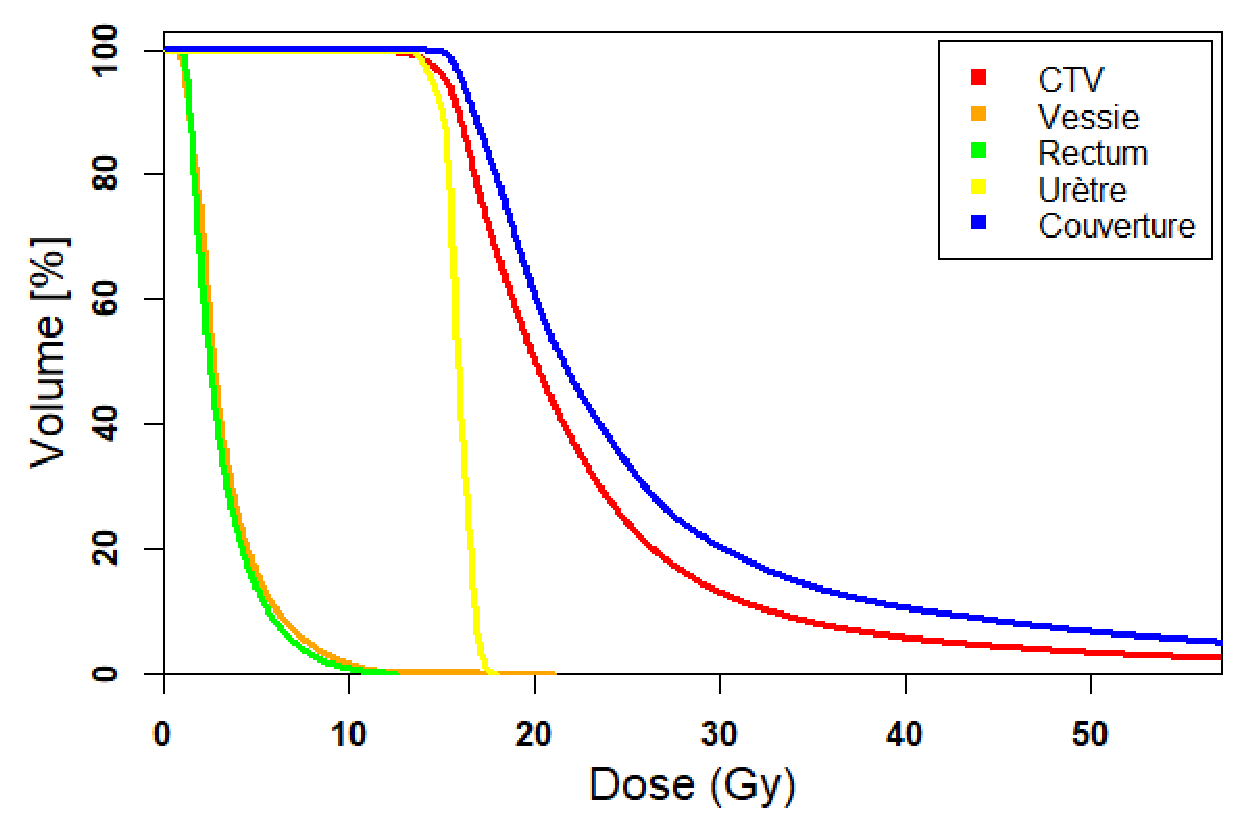
\includegraphics[width=9.0cm, height=6.5cm]{DVH.eps}
\caption{\label{DVH}Exemple d’un DVH cumulatif pour une prostate traitée en curiethérapie HDD en une séance de 15Gy, en complément à la radiothérapie externe (boost).}
\end{figure}
%
L’inconvénient majeur de cet outil est l’absence totale de l’information spatiale, c’est-à-dire, aucune localisation géométrique des volumes extraits des DVHs n’est possible, d’où la complémentarité de cet outil avec ceux décrits précédemment.
%
\newpage
\section{Description du projet de recherche}
Le présent projet porte sur la curiethérapie de la prostate HDD dont le développement a eu un regain d’intérêt dans les années 1980, après que Halm et al. \cite{Holm2002} aient démontré dans leurs travaux que la radiographie ultrason transrectal pouvait être utilisée pour guider la réalisation des implants prostatiques avec une meilleure précision. Cette approche est utilisée aujourd’hui par plusieurs centres de radiothérapie pour les traitements en curiethérapie HDD avec les projecteurs de sources équipés de sources d’Iridium-192 \cite{Stromberg, Mate, Borghede, Hoskin, Demanes, Blasko}. La réalisation des objectifs cliniques en termes de conformité de la dose au volume cible et limitation de la dose aux tissus et organes à risques (OARs) \nomenclature{OAR}{Organe à risque (Organs At Risk)} dépend d’une part, de la précision avec laquelle les cathéters sont implantés dans la glande, et d’autre part, de la méthode d’optimisation utilisée par le TPS. Les premières méthodes d’optimisation traditionnelles les plus utilisées étaient l’optimisation géométrique et l’optimisation par points de dose \cite{Ezzel, Thomadsen, Edmundson1, Edmundson2}. Un des points caractéristiques communs à ces deux méthodes est la nécessité d’une forte interaction entre le planificateur et le TPS, \nomenclature{TPS}{Système de planification de traitement (Treatment Planning Systems)} car ce dernier doit essayer plusieurs combinaisons de positions actives au sein de chaque cathéter, ainsi que les poids respectifs associés à chacune des positions, afin d’obtenir une distribution de dose satisfaisante, c’est-à-dire, qui respecte les objectifs cliniques. Cette dépendance, non seulement augmente la durée de la planification, mais conduit aussi à un plan final dont la qualité dépend du jugement et de l’expérience du planificateur. Le développement de la planification inverse avec l’algorithme IPSA \cite{ELessard, LessardP, Lessard2004} a permis l’automatisation de certaines tâches. Cette classe d’algorithme est caractérisée par la définition d’une fonction de coût qui reflète les objectifs cliniques et les contraintes de dose aux tissus sains (section \ref{sssec:optimis}). L’interaction entre le planificateur et le TPS se trouve ainsi réduite, car l’algorithme IPSA détermine automatiquement les positions à activer au sein de chaque cathéter (dwell positions), ainsi que le temps d’arrêt à chacune des positions (dwell time). Cependant, le processus d’optimisation demeure itératif et la qualité du plan reste dépendante du jugement du planificateur et de son expérience, puisque la solution optimale calculée par l’algorithme reste dépendante de la combinaison des pénalités que le planificateur a imposées à chaque objectif et/ou contrainte. Les outils d’évaluation d’un plan (isodose, DVH, etc.) \nomenclature{DVH}{Histogrammes doses-volumes (Dose Volume Histogram)} reposent essentiellement sur les recommandations de la couverture de dose dans le volume cible, et la limite de celle-ci aux OARs, recommandations contenues dans les publications de certains organismes internationaux tels que le RTOG 0924 \cite{ RTOG} \nomenclature{RTOG}{ Radiation Therapy Oncology Group}  ou de l’American Brachytherapy Society (ABS) \nomenclature{ABS}{American Brachytherapy Society}\cite{ABS}. Ces recommandations sont basées sur les études d’inférence statistiques, et donc, ne prennent pas en compte les variations des paramètres géométriques inter-patients qui ont un impact sur le compromis à réaliser, entre la couverture du volume cible et la minimisation de la dose aux OARs. De plus, il n’existe aucun outil objectif permettant au planificateur de juger de la qualité du compromis obtenu dans l’atteinte des objectifs cliniques. On pourrait donc penser de ce qui précède que, quelles que soient la méthode d’optimisation utilisée et l’expérience du planificateur, le plan de traitement obtenu suite à un tel processus de planification, bien qu’il soit conforme aux objectifs cliniques, n’est pas nécessairement le plus optimal qu’il serait possible d’obtenir. Les insuffisances décrites ci-dessus suggèrent la nécessité de développer de nouveaux outils d’aide à la planification, d’où l’intérêt de ce projet dont l’objectif est d’introduire un nouveau concept de contrôle qualité en curiethérapie de la prostate HDD, grâce à l’analyse de frontière stochastique (AFS) \nomenclature{AFS}{Analyse de Frontière Stochastique} qui est une méthode économétrique \cite{Dennis}. L’application de l’AFS dans ce contexte conduira à la construction des modèles d’aide à l’optimisation des plans, grâce aux paramètres géométriques inter-patients. Ces modèles auront également un pouvoir prédictif sur les paramètres dosimétriques d’intérêt qui guident le processus de planification. Plusieurs études réalisées en radiothérapie par modulation d’intensité (IMRT) \nomenclature{IMRT}{Radithérapie par modulation d’intensité (Intensity Modulated Radiation Therapy)} ont montré que de telles corrélations (dose-paramètres géométrique) étaient possibles et pouvaient conduire à l’amélioration de la qualité des plans de traitement en IMRT \cite{LachanceB, KevinLM, MargieAH, Marie-Chantal}. Les modèles développés constitueront également un outil objectif dans l’évaluation de la qualité du compromis obtenu à la fin d’un processus de planification (couverture du volume cible vs minimisation de la dose aux OARs).
%
\section{Organisation du mémoire}
%\addcontentsline{toc}{section}{Organisation du mémoire}
Le présent travail est organisé en quatre parties. Après une introduction (chapitre 1) qui présente brièvement l'origine de la radiothérapie, et particulièrement la curiethérapie, les concepts d'assurance et contrôle qualité, la présentation du cancer de la prostate (incidence, mortalité, diagnostic et aspects dosimétriques), et la description des objectifs du présent projet, suivra le chapitre 2 consacré à la présentation du formalisme de l’analyse de frontière stochastique et son exploitation dans le cadre de ce projet pour l’optimisation des plans en curiethérapie de la prostate HDD. Un article résumant les résultats principaux de ce travail pour soumission au Brachytherapy Journal fait partie du chapitre 3, et une conclusion ainsi que des développements futurs du projet pour ces aspects cliques clôturent ce travail dans sa quatrième partie.
%          % introduction
\chapter{Modèles d'analyse de frontière stochastique pour l'optimisation des plans en curiethérapie HDD} \label{chapitre2} %  numéroté
\lettrine[nindent=0em,lines=2]{L}{}a Garantie de la qualité d’un traitement en curiethérapie nécessite la mise en place d’un programme de contrôle et de maintenance à plusieurs étages du processus de traitement. Rappelons de façon succincte que la qualité d’un traitement se mesure par l’habilité à traduire correctement les objectifs du traitement défini par le radio-oncologue en dose prescrite au volume cible tout en assurant la protection des OARs alentour. Sans être exhaustif, les grandes étapes permettant d’assurer et de maintenir la qualité des traitements consistent en: (1) la vérification des caractéristiques physiques des sources, (2) la vérification du fonctionnement des projecteurs de source ainsi que, (3) la vérification des systèmes de planification des traitements.
%
\begin{itemize}[label=\textbullet, font=\LARGE]
\item \textbf{Vérification des caractéristiques physiques}\newline
La vérification du certificat d’étalonnage des sources est une étape importante dans la démarche du maintien de la qualité. En effet, plusieurs études menées dans le but de comparer les caractéristiques physiques des sources fournies par les constructeurs à celles réellement mesurées ont permis de déceler des variations non négligeables; ces variations sont à l’origine des recommandations sur la vérification systématique du certificat de calibration des sources dès leur réception\cite{Baltas@1999, Elfrink@2002, Venselaar@1995}. Cette vérification peut porter, entre autres, sur la nature de la source proprement dite, le contrôle de conformité du certificat de calibration, l’homogénéité ainsi que la vérification de l’activité de chacune des sources avec une tolérance dans la variabilité de ± 10\% \cite{HaieMeder@2002}. La plupart des centres, en occurrence l’HDQ, utilisent les valeurs mesurées au sein de leurs services comme valeurs de référence dans le système de dosimétrie.
\\
%
\item \textbf{Vérification du fonctionnement des projecteurs de sources }\newline
Les projecteurs de sources jouent deux rôles fondamentaux dans le processus de planification, notamment, la radioprotection et de la dosimétrie. En curiethérapie HDD, ils sont responsables d’exécuter la programmation de la position de la source dans les différents cathéters implantés dans le CTV. Les tests recommandés pour assurer le bon fonctionnement d’un projecteur de source sont divers, parmi lesquels, la vérification de la précision de la position de la source au sein des cathéters d’une part \enquote{dwell position}, et d’autre part, la vérification sur la sélection du canal approprié tel que programmé lors de la planification. Le groupe de travail de l’AAPM TG-56 \cite{Nath@1997} recommande une précision sur la position de la source de ± 2 mm relative au système de référence de l’applicateur, et une tolérance de ± 2\% dans la vérification des temps d’irradiation à chacune des positions \enquote{dwell time}.
%
\item \textbf{Vérification des systèmes de planification des traitements}\newline
La vérification indépendante du calcul optimisé de la dose par un TPS avec une technique manuelle de calcul permettant de détecter des erreurs significatives avant chaque traitement constitue toujours un défi pour les physiciens, compte tenu de la contrainte sur le délai qui sépare le processus de planification et la délivrance de la dose au patient. Plusieurs approches de vérification ont été proposées dans la littérature \cite{Thomadsen@1992, Kubo@1992, Saw@1998} dont une consiste à considérer un point assez éloigné de l’implant de telle sorte que l’effet cumulatif des sources dans l’implant soit assimilable à une source ponctuelle; l’approximation de l’inverse carré de la distance peut ainsi être appliquée pour le calcul manuel afin de comparer le résultat à la valeur prédite par le TPS. En 2006, Rupak et al.\cite{Rupak@2006} ont proposé une méthode de vérification basée sur les DVHs. Bien que la précision de l’algorithme d’optimisation implémenté dans le TPS ait été évaluée lors de la phase du commissionnement de ce dernier, ce calcul indépendant permet cependant de vérifier, entre autres que les caractéristiques physiques des sources qui ont servi au calcul de la dose sont correctement prises en compte au cours de la planification (nature de la source, activité, date de traitement, décroissance radioactive), et qu’un éventuel bug dans le TPS n'a pas affecté le calcul de la dose.
\end{itemize}
%
La présentation succincte ci-dessus ne couvre certainement pas tous les aspects du contrôle de la qualité des plans en curiethérapie HDD, mais donne une idée sur l’approche classique recommandée dans la littérature et unanimement adoptée par les centres de radio-oncologie pour garantir la qualité des traitements. Cette approche est cependant complètement différente de celle adoptée dans le présent travail, bien que celle-ci se focalise également sur l’aspect de l’amélioration de la qualité des plans. L’approche basée sur l’AFS sur laquelle s’appuie le présent projet est un nouveau concept que nous introduisons en physique et doit être perçue comme complément à l’approche classique brièvement présentée ci-dessus; les deux ayant pour objectif global de garantir le contrôle tumoral sans délivrer de doses inutiles aux OARs.
%
\section{Formalisme de frontière stochastique}
L’analyse de frontière stochastique (AFS) \nomenclature{AFS}{Analyse de Frontière Stochastique} est une méthode développée en économie pour évaluer les performances d’une entreprise. La méthode repose sur la modélisation du processus de production permettant de prédire la quantité maximale d’extrants qui peut être produite, sur la base d’un vecteur d’intrants pour une technologie donnée. Aigner et al.\cite {aigner@2004} et Meeusen et al.\cite {meeusen@2004} furent les premiers pionniers à s’investir dans ce processus de modélisation, en proposant indépendamment et simultanément, un modèle de frontière qui prend en considération à la fois les éléments considérés comme exogènes au processus de production d’une entreprise, et les éléments représentés par l’efficience technique. La représentation mathématique d’une telle approche est donnée par l’équation \eqref{eqn:Frontiere},
%
\begin{equation}\label{eqn:Frontiere}
	y_{i} = f(x_{i}; \beta) + \epsilon_{i},  \quad \epsilon_{i} = v_{i} \mp u_{i}
\end{equation}
%
dans laquelle $y_{i} $ est un vecteur d’extrants pour la firme $ i $, $x_ {i} $ un vecteur d’intrants et $\beta $, un vecteur de paramètres à déterminer au cours du processus d’optimisation. Le terme d’erreur $\epsilon_ {i} $ est décomposé en deux composantes, un terme $v_{i}$ purement aléatoire et symétrique modélisant tous les facteurs qui ne sont pas sous le contrôle de l’entreprise, mais qui peuvent influencer la productivité de celle-ci (température, prix des matières premières, fluctuation du cours des actions, ou tout simplement la chance). Les $v_{i} $ sont supposés être iid selon N$(0, \sigma^{2}_{v})$. Cette composante aléatoire peut avoir une influence positive ou négative dans la productivité de l’entreprise en la déplaçant respectivement au-dessus ou au-dessous de sa frontière. $u_{i}\geq 0$ est un terme d’efficience technique associé aux facteurs contrôlables par la firme (efficacité ou la compétence des employés). $u_{i}$ est supposé indépendant de $v_{i}$ et distribué selon une loi normale tronquée positive, $N^{+}(0, \sigma^{2}_{u})$. Si les facteurs contrôlables par la firme sont correctement gérés, celle-ci devrait atteindre sa productivité maximale donnée par la frontière [$f(x_{i}; \beta) + v_{i}$]. Les signes $\mp$ dans l’équation \eqref{eqn:Frontiere} correspondent respectivement à une frontière de production et à une frontière de coût. La frontière de production prédit le maximum d’extrants sur la base d’un ensemble d’intrants, alors que la frontière de coût est associée à la minimisation des coûts de la production, c’est-à-dire, elle détermine le maximum de dépense devant être associée à une productivité maximale donnée. La forme analytique de la fonction $f(x_{i}; \beta)$ la plus utilisée dans la littérature est la fonction de Cobb-Douglas \cite{cobb@2004} donnée par l’équation \eqref{eqn:Chp2Cobb}:
%
\begin{equation}\label{eqn:Chp2Cobb}
	y_{i} = c \times \prod_{i} x^{\propto_{i}}_{i}
\end{equation}
%
dans laquelle $c > 0$  et $\alpha_{i} \in \Re$. La figure \ref{FrontiereCTV} ci-dessous illustre un exemple d’une frontière de production. La région mise en évidence en jaune identifie les firmes qui sont économiquement efficientes (productivité maximale atteinte pour un même vecteur d’intrants).
%
\begin{figure}[ht!]
\centering
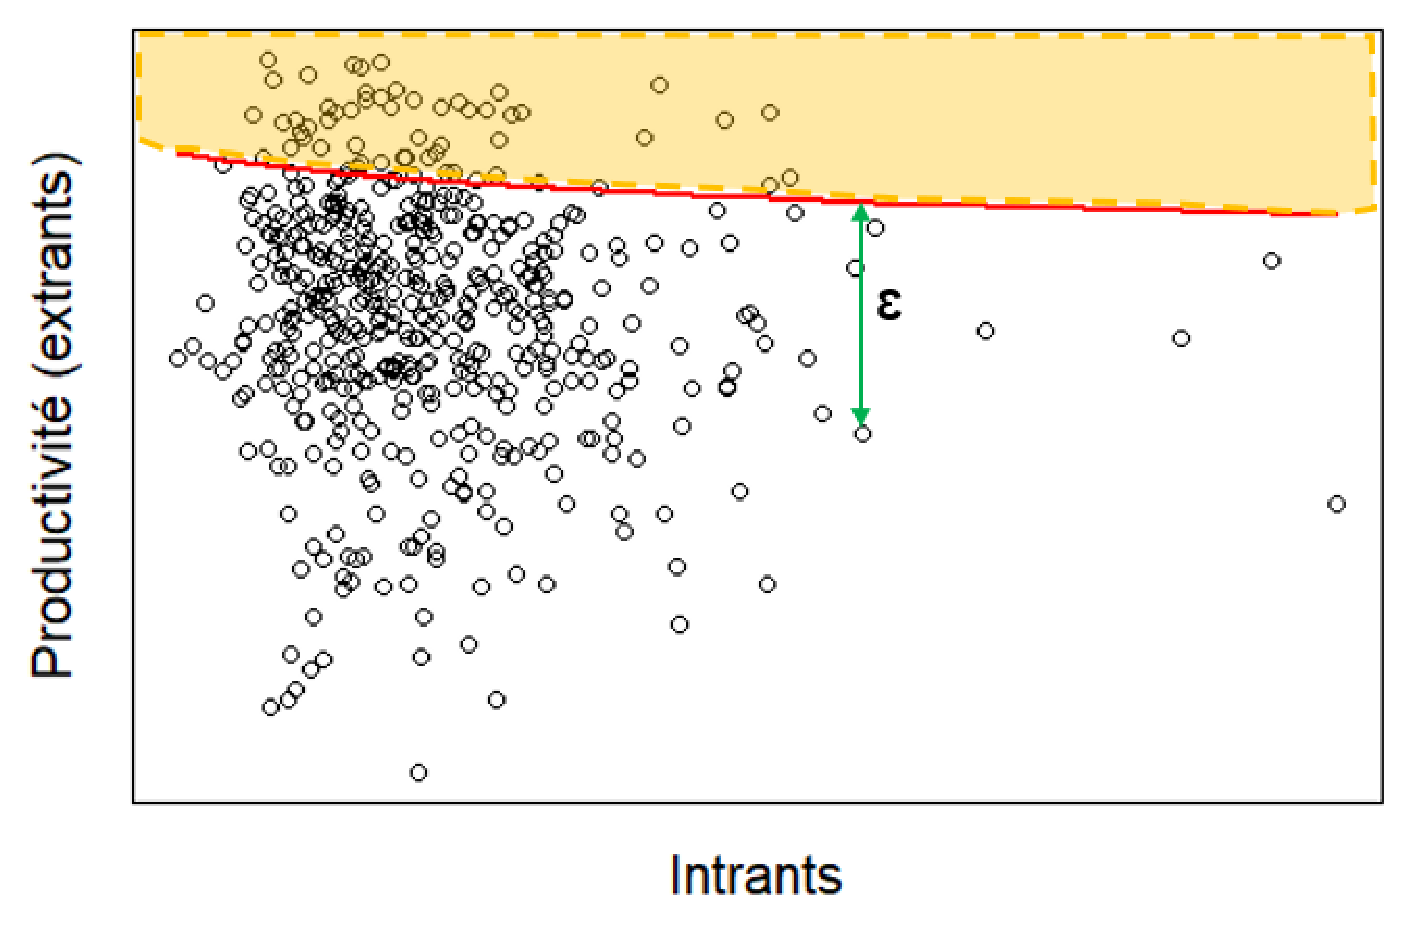
\includegraphics[width=8.5cm,height=5.8cm]{FrontiereCTV}
\caption{\label{FrontiereCTV} Illustration graphique de la frontière de production. $\epsilon$ est la distance entre la production d'une entreprise donnée par rapport à sa valeur prédite par la frontière.}
\end{figure}
%
La densité de probabilité conjointe, $f(u, v)$, sous l'hypothèse de l'indépendance des deux distributions $(u, v)$ est donnée par la relation:
%
\begin{equation}\label{eqn:fs1a}
f(u, v)=\frac{1}{\pi\sigma_{u}\sigma_{v}}exp\left[-\left(u^{2}/2\sigma^{2}_{u}\right)-\left(v^{2}/\sigma^{2}_{v}\right)\right]
\end{equation}
%
Dans le cas d'une frontière de production, en remplaçant $v$ par $u-\epsilon$ dans l'équation \ref{eqn:fs1a} et en intégrant dans le domaine de variabilité de $u$, c'est-à-dire, $[0, +\infty[$, on obtient la densité de probabilité de $\epsilon$ donnée par l'équation (\ref{eqn:fs2a}),
%
\begin{equation}\label{eqn:fs2a}
f\left(\epsilon_{i}\right) = \frac{2}{\sigma\sqrt{2\pi}}\left[1-\Phi\left(\frac{-\epsilon_{i}\lambda}{\sigma}\right)\right]exp\left(\frac{-\epsilon^{2}_{i}}{2\sigma^{2}}\right)
\end{equation}
%
dans laquelle, $\sigma = \sqrt{\sigma^{2}_{u}+\sigma^{2}_{v}}$ représente la largeur de la distribution, $\lambda=\sigma_{u}/\sigma_{v}$ son asymétrie, ou une mesure de la variabilité relative des deux sources d’erreurs. $\Phi\left(.\right)$ est la fonction de répartition d’une loi normale centrée réduite. Les différentes valeurs de $\lambda$ déterminent la nature de la frontière. Lorsque $\lambda = 0$, seule la composante aléatoire gouverne la distribution donnée par l’équation (\ref{eqn:fs2a}) et la frontière devient un simple ajustement. Une valeur élevée de $\lambda$ ($\lambda \rightarrow +\infty$) signifie que les facteurs qui sont sous le contrôle de l’entreprise sont dominants dans le manque de la production maximale, la frontière prend alors un caractère déterministe et la distribution de l'équation (\ref{eqn:fs2a}) devient celle d’une loi normale tronquée négative. L’espérance mathématique et la variance de $\epsilon$ sont décrits respectivement par les équations (\ref{eqn:fs3a}) et (\ref{eqn:fs4a}),
%
\begin{equation}\label{eqn:fs3a}
E\left(\epsilon\right)=E\left(u\right)=-\sqrt{\frac{2}{\pi}}\sigma_{u}
\end{equation}
%
\begin{equation}\label{eqn:fs4a}
V\left(\epsilon\right)=V\left(u\right)+V\left(v\right)=\left(\frac{\pi-2}{\pi}\right)\sigma^{2}_{u}+\sigma^{2}_{v}
\end{equation}
%
Les équations similaires pour une frontière de coût peuvent être déduites des équations (\ref {eqn:fs1a}-\ref{eqn:fs4a}) en y remplaçant $\epsilon $ par $ -\epsilon $. La figure \ref {DensiteProb} ci-dessous illustre la forme de la densité de probabilité de la variable $\epsilon$ donnée par l'équation (\ref{eqn:fs2a}), respectivement pour une frontière de production (a) et une frontière de coût (b).
%
\begin{figure}[ht!]
  \centering
  \subfloat[Frontière de production]{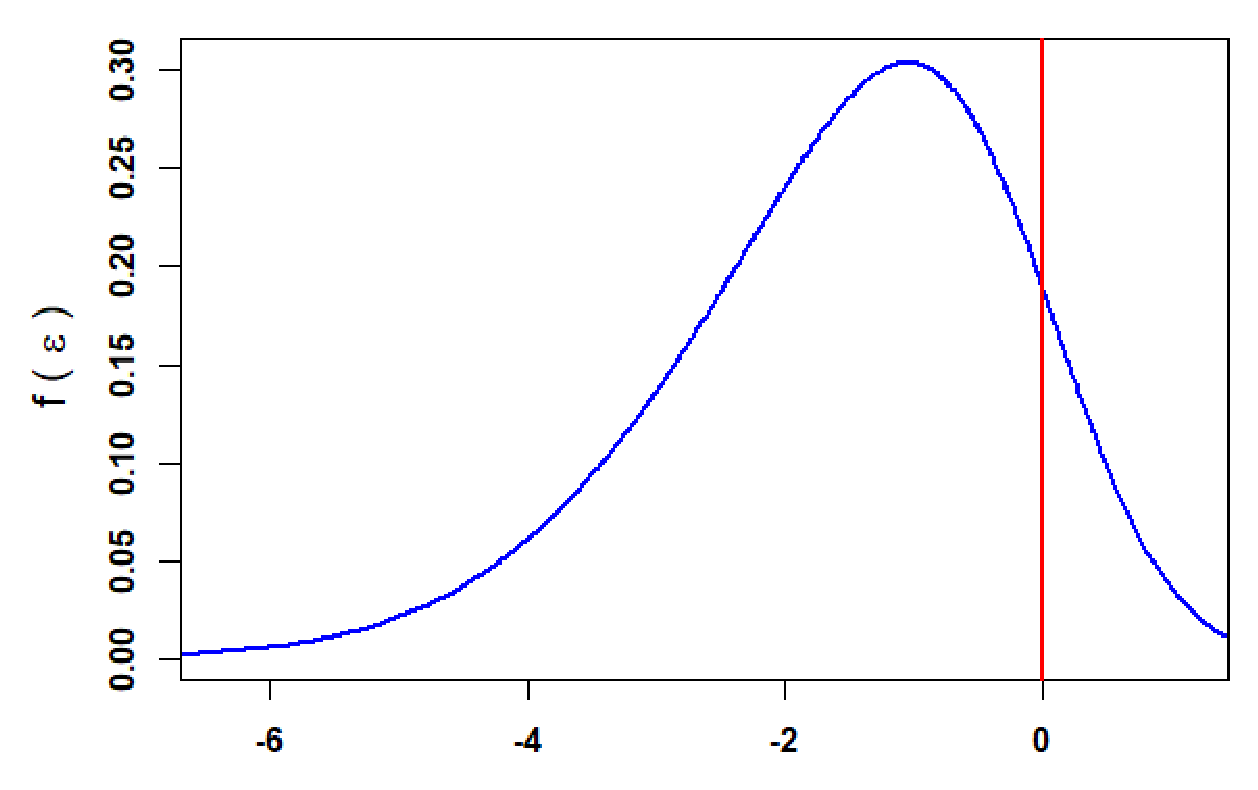
\includegraphics[width=7.1cm,height=5.2cm]{DensiteProbA}\label{fig:f1}}
  \hspace{0.5cm}
  \subfloat[Frontière de coût ]{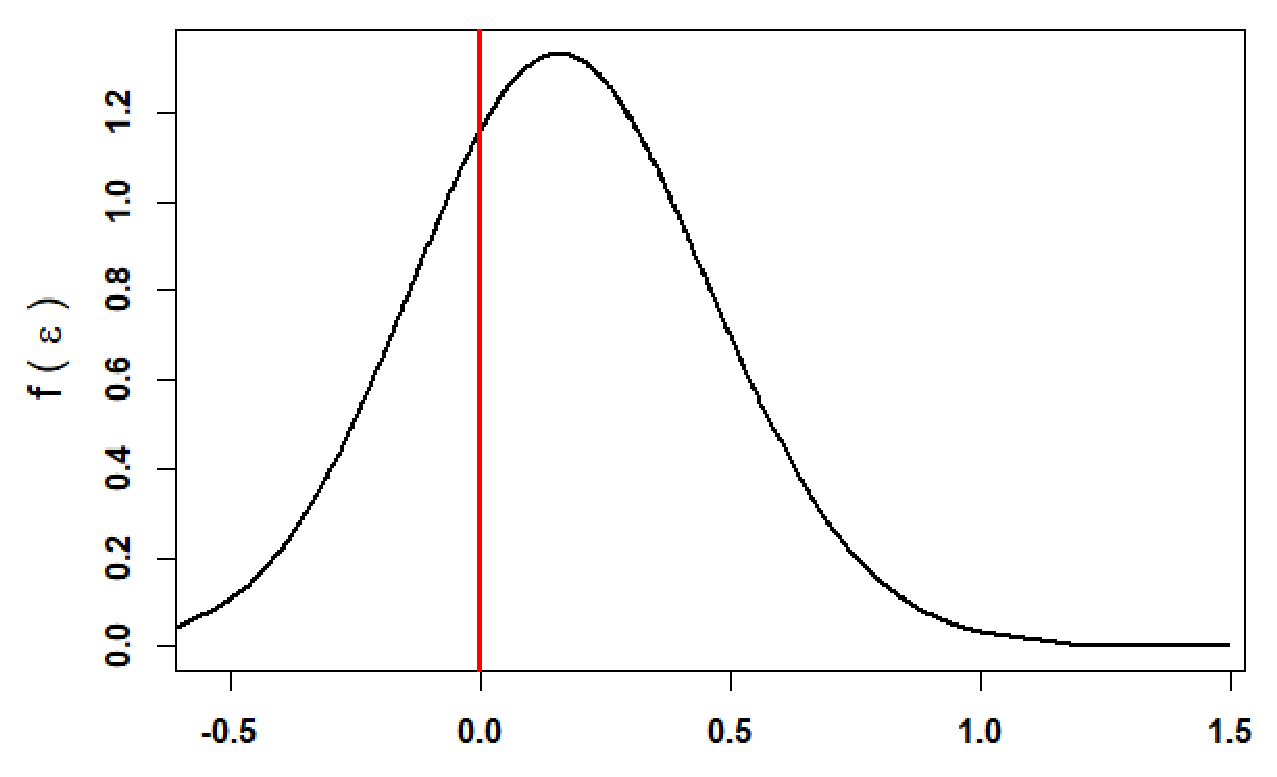
\includegraphics[width=7.2cm,height=5.2cm]{DensiteProbB}\label{fig:f2}}
\caption{\label{DensiteProb} Illustration d'une distribution tronquée négative (a) et tronquée positive (b). Les deux cas correspondent au scénario pour lequel la composante déterministe $u$ de $\epsilon$ est dominante.}
\end{figure}
%
L’utilisation de ce formalisme d'AFS dans le contexte de l’optimisation des plans en curiethérapie HDD repose dans le développement des modèles de frontière de production pour les paramètres dosimétriques que l’on cherche à maximiser au cours de la planification (couverture du CTV), et de frontières de coût pour ceux qui sont sujets à la minimisation (OARs). La forme analytique de la frontière présentée dans l’équation (\ref{eqn:Chp2Cobb}) a été modifiée dans son application. En effet les paramètres géométriques $x_{i}$ de cette équation ont été remplacés par un profil géométrique construit sous forme d’une combinaison linéaire desdits paramètres, suivant l’équation (\ref{eqn:Chp2Cobb2})
%
\begin{equation}\label{eqn:Chp2Cobb2}
	y_{i} = c\times \left(\sum_{i}\beta_{i}x_{i}\right)^{\alpha}
\end{equation}
%
Le passage de l’équation (\ref{eqn:Chp2Cobb}) à l’équation (\ref{eqn:Chp2Cobb2}) qui s’est fait sans perte d’informations contenues dans les modèles ($\sigma_{u}, \sigma_{v}$), présente l’avantage de visualiser les frontières dans un graphique à deux dimensions lorsque le nombre de paramètres géométriques impliqué dans le processus de modélisation est supérieur à deux.
%
\section{Application à l'optimisation des plans en curiethérapie de la prostate HDD}
\subsection{Acquisition des échantillons}
La première phase de la modélisation a consisté en l’acquisition de deux échantillons indépendants. Un premier échantillon de 495 patients qui a servi dans la construction des modèles, correspond aux patients traités dans la plage mars 2013 - juillet 2016, et un deuxième échantillon de 100 patients traités en 2011 qui a servi de test. Les deux échantillons sont des patients traités en curiethérapie de la prostate HDD, en une fraction de 15 Gy, en complément après une radiothérapie externe. L'optimisation de la dosimétrie de ces patients s'est faite avec l'algorithme IPSA implémenté dans le TPS Oncentra Brachy (Elekta - Brachy, Veenendaal, The Netherlands).
%
\subsection{Description et extraction des paramètres géométriques} \label{Parag}
\subsubsection{Volume des structures (CTV, OARs)}
L’extraction des volumes des différentes structures (CTV, vessie, rectum et urètre) a été faite manuellement à partir du TPS pour les 100 premiers patients du premier échantillon. Le programme 3D Slicer a été utilisé pour faciliter l’extraction de ces volumes pour le reste des plans (premier et deuxième échantillon). L’extraction des paramètres géométriques s’est effectuée en deux étapes. Dans la première étape, les DVH des différents plans ont été extraits manuellement à partir de 3D Slicer et un script sous Python a permis l’automatisation de l’extraction des paramètres géométriques sur lesdits DVH. Le niveau de précision des volumes ainsi calculés a d’abord été évalué en comparant les valeurs calculées avec ceux extraits manuellement du TPS pour les 100 premiers patients. Pour le CTV, la vessie et le rectum, les écarts relatifs moyens des différents volumes calculés, entre le TPS et 3D Slicer sont respectivement de de 2,02\% ($\sigma = 0,578 $), 1,14\% ($\sigma = 0,544 $) et 1,90\% ($\sigma = 1,11 $). Pour le volume de l’urètre, l’écart absolu moyen entre 3D Slicer et le TPS est de 0,14 ($\sigma = 0,024 $). L’application des différents modèles de régression présentés dans la figure \ref{ModeleRegres} pour le calcul des volumes du CTV, du volume de la vessie et du volume du rectum a amélioré la précision des calculs, c’est-à-dire, la moyenne des écarts relatifs est passée des valeurs citées précédemment à 0,35\% ($\sigma = 0,24 $), 0,45\% ($\sigma = 0,55 $) et 0,93\% ($\sigma = 1,42 $), respectivement. L’écart absolu moyen pour le volume de l’urètre après correction est de 0,014 ($\sigma = 0,01 $). Ces modèles de régression ont été appliqués pour corriger toutes les valeurs des paramètres géométriques extraits des DVHs pour le reste des plans des deux échantillons.
%
\begin{figure}%[ht!]
  \centering
  \subfloat{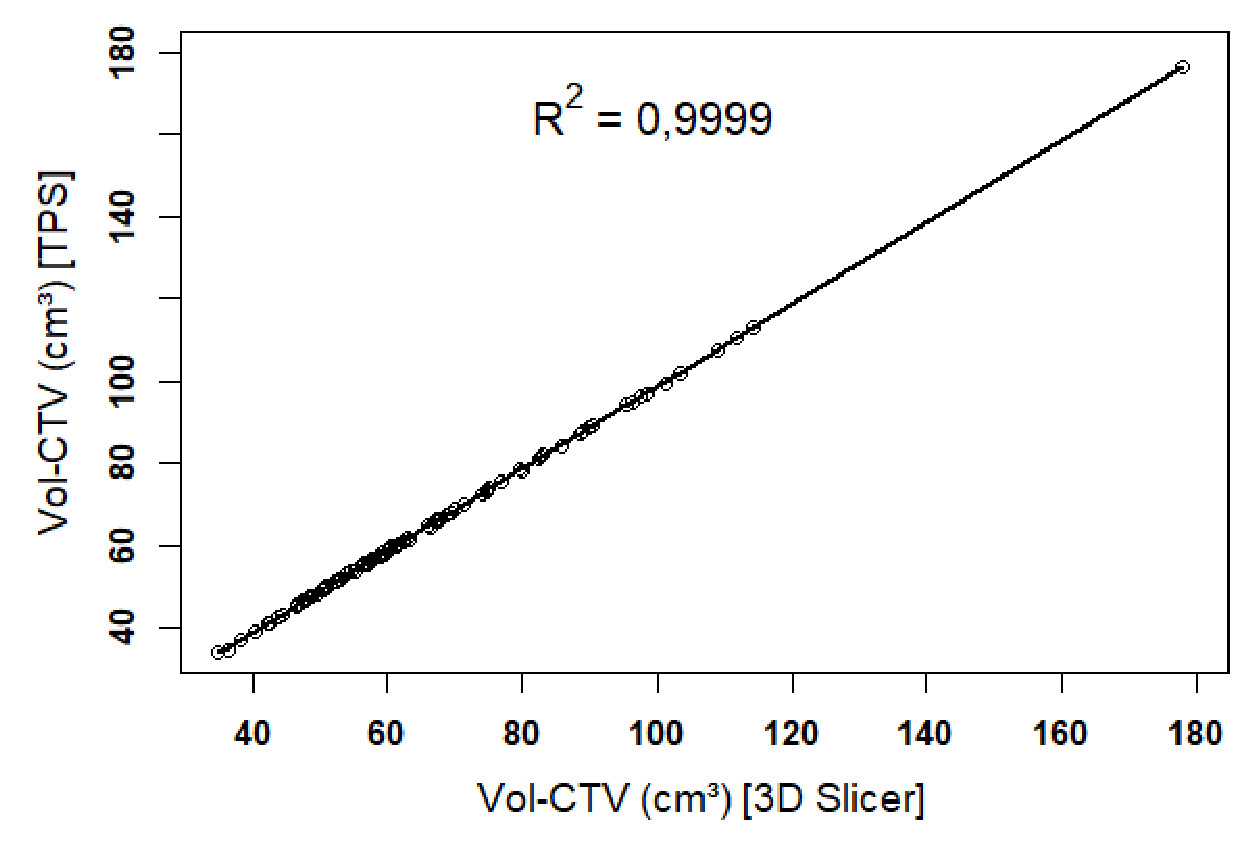
\includegraphics[width=7.2cm,height=5.2cm]{RegresCTV}\label{fig:RegresCTV}}
  \hspace{0.5cm}
  \subfloat{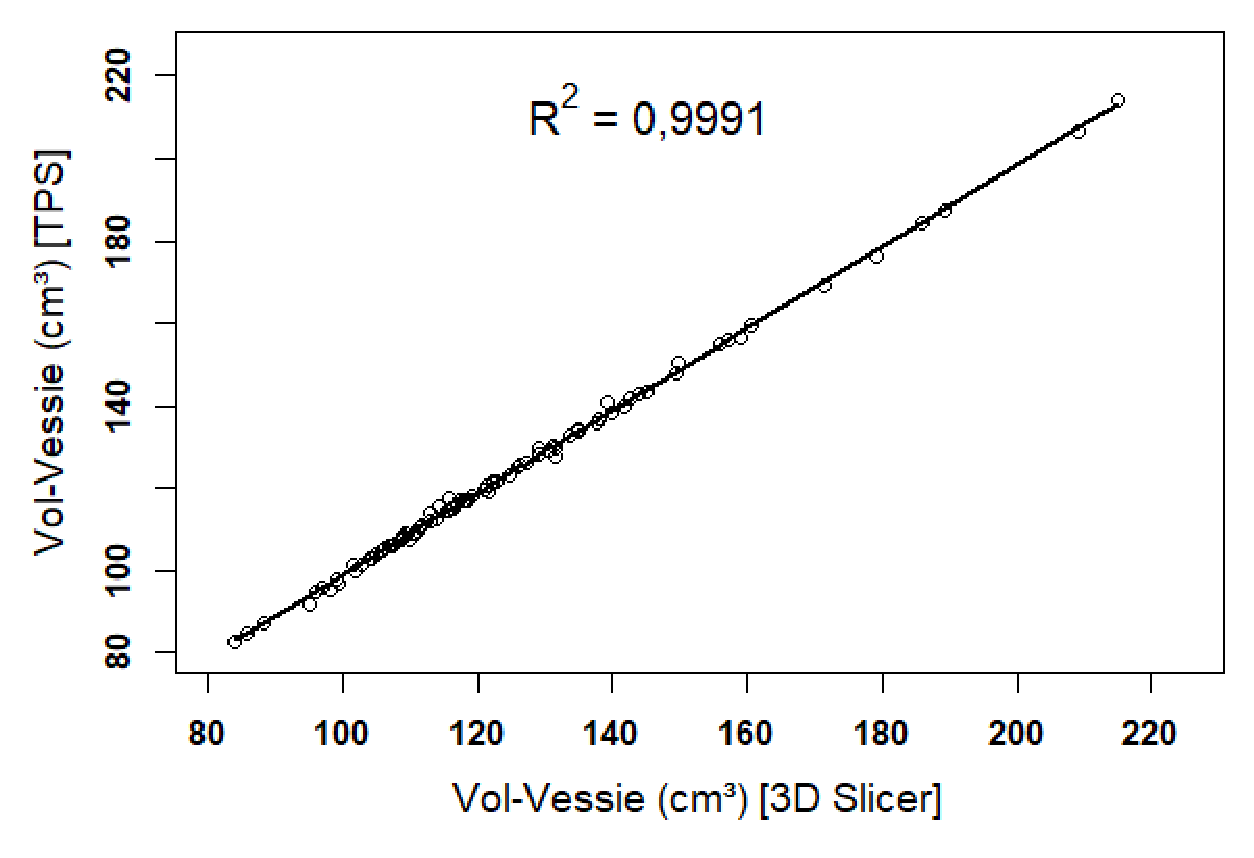
\includegraphics[width=7.2cm,height=5.2cm]{RegresVessie}\label{fig:RegresVessie}}
  \hspace{0.5cm}
  \subfloat{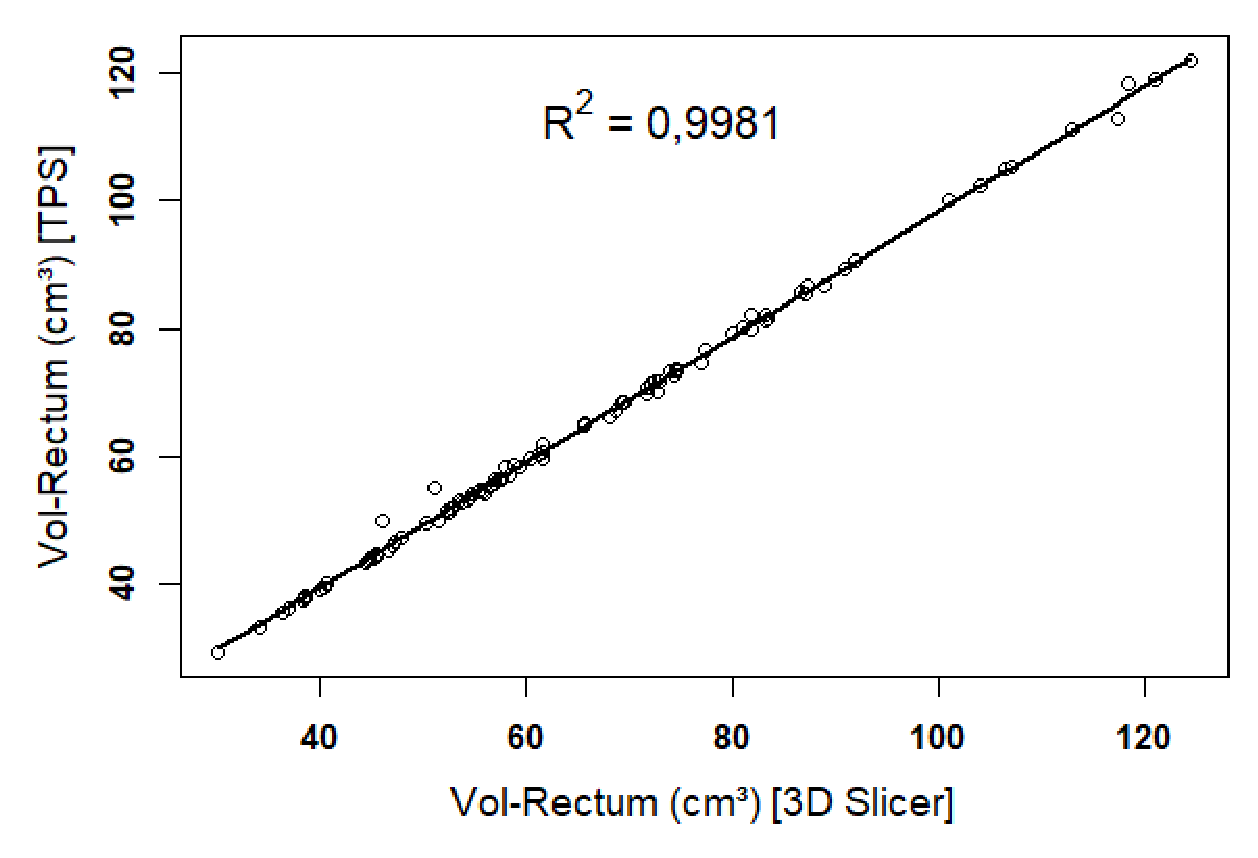
\includegraphics[width=7.2cm,height=5.2cm]{RegresRectum}\label{fig:RegresRectum}}
  \hspace{0.5cm}
  \subfloat{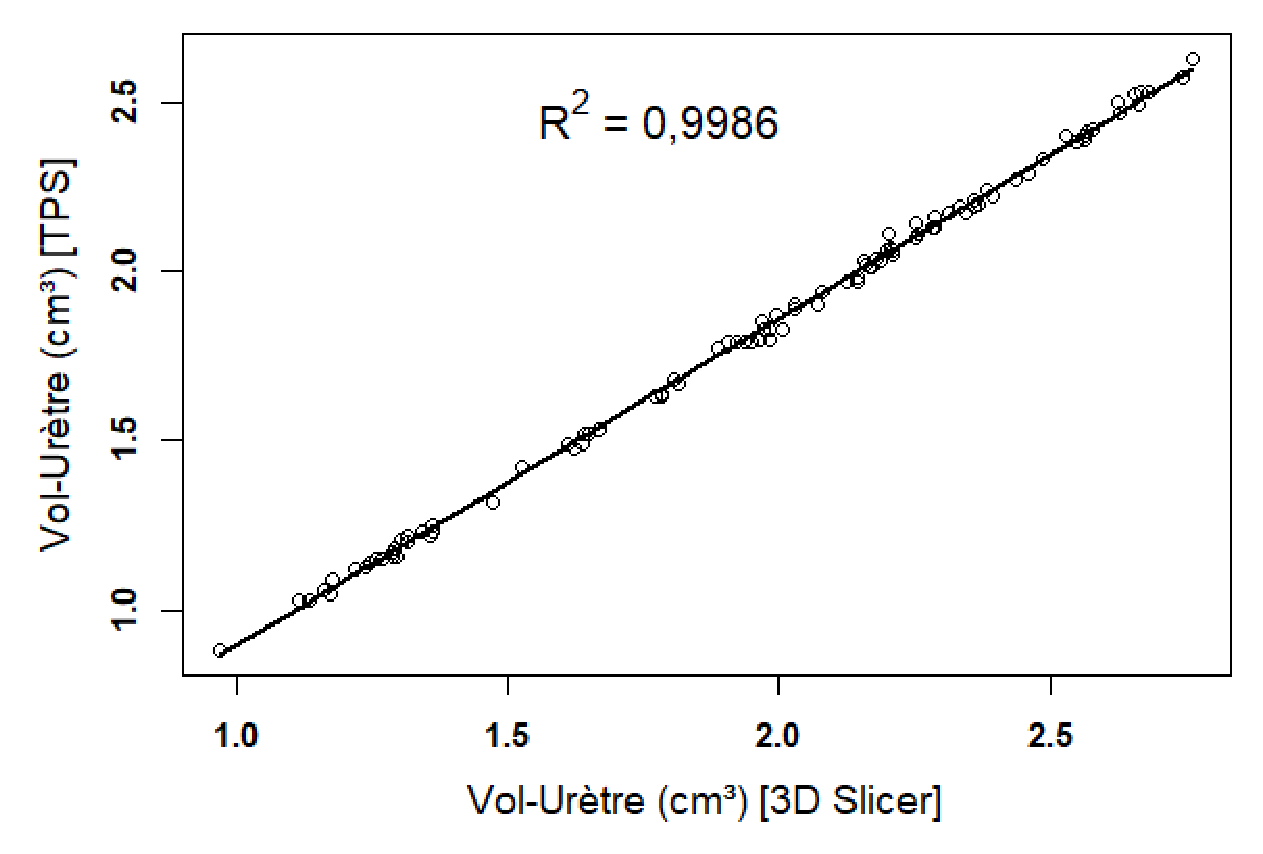
\includegraphics[width=7.25cm,height=5.2cm]{RegresUretre}    \label{fig:RegresUretre}}
  %\hspace{0.5cm}
\caption{\label{ModeleRegres} Résultats des modèles de régressions linéaires construits à partir des volumes calculés par 3D Slicer.}
\end{figure}
%
\subsubsection{Distance de Hausdorff CTV-OARs}
En mathématiques, et plus précisément en topologie, la distance de Hausdorff est un outil qui mesure l’éloignement de deux sous-ensembles d’un espace métrique sous-jacent. Celle-ci porte le nom de son inventeur, le mathématicien allemand Felix Hausdorff. Cette distance est tributaire de plusieurs propriétés qui lui confèrent son utilisation, entre autres, dans la reconnaissance des formes, la quantification des dissemblances entre deux formes géométriques, ou dans la numérisation des images. Elle a été utilisée dans le contexte du présent projet pour quantifier la distance entre le CTV et chaque OAR (vessie, rectum et urètre). Elle présente l’avance par rapport à la distance euclidienne, de quantifier la proximité relative entre deux structures tout en tenant compte de leurs formes respectives. Du point de vue formel, si on considère deux ensembles A et B bornés et non vides, la distance de Hausdorff entre les deux ensembles est le maximum de la fonction définie par l’équation (\ref{eqn:Hausdorff1}),
%
\begin{equation}\label{eqn:Hausdorff1}
	h (A, B) = max_{a\in A}\left\{min_{b\in B}\left\{d (A, B)\right\}\right\}
\end{equation}
%
dans laquelle, d (A, B) est n’importe quelle métrique entre A et B en général et en particulier, une distance euclidienne entre les deux ensembles dans le présent projet. Il convient cependant de souligner que la distance de Hausdorff est une distance orientée, c’est-à-dire, dans la plupart des cas, h (A, B) $\neq$ h (B, A), d’où la formulation plus générale donnée dans l’équation (\ref{eqn:Hausdorff2}),
%
\begin{equation}\label{eqn:Hausdorff2}
	H (A, B) = max\left\{h (A, B), h (A, B)\right\}
\end{equation}
%
\subsubsection{Divergence moyenne des cathéters}
Sous guidage échographique, les cathéters implantés dans le volume cible présentent généralement une certaine divergence entre elles; cette divergence, volontaire ou non, influence la dosimétrie. Ce paramètre a été évalué en deux étapes. Premièrement, les données permettant de reconstruire les cathéters ont été extraites des fichiers DICOM et les cathéters ont été reconstruits (figure \ref{Catheters}A), puis découpés aux dimensions de la prostate (figure \ref{eqn:Hausdorff2}B). Les points rouges représentent les positions activées au sein de chaque cathéter. Deuxièmement, la divergence moyenne des cathéters a été évaluée en calculant la pente moyenne; celle-ci a été échantillonnée dans chaque cathéter sur tous les deux (respectivement, trois points), si le nombre de points permettant de reconstruire ledit cathéter est pair (respectivement, impair). Une divergence moyenne globale a été ensuite déduite en moyennant la pente dans l'ensemble des cathéters.
%
\begin{figure}[ht!]
\centering
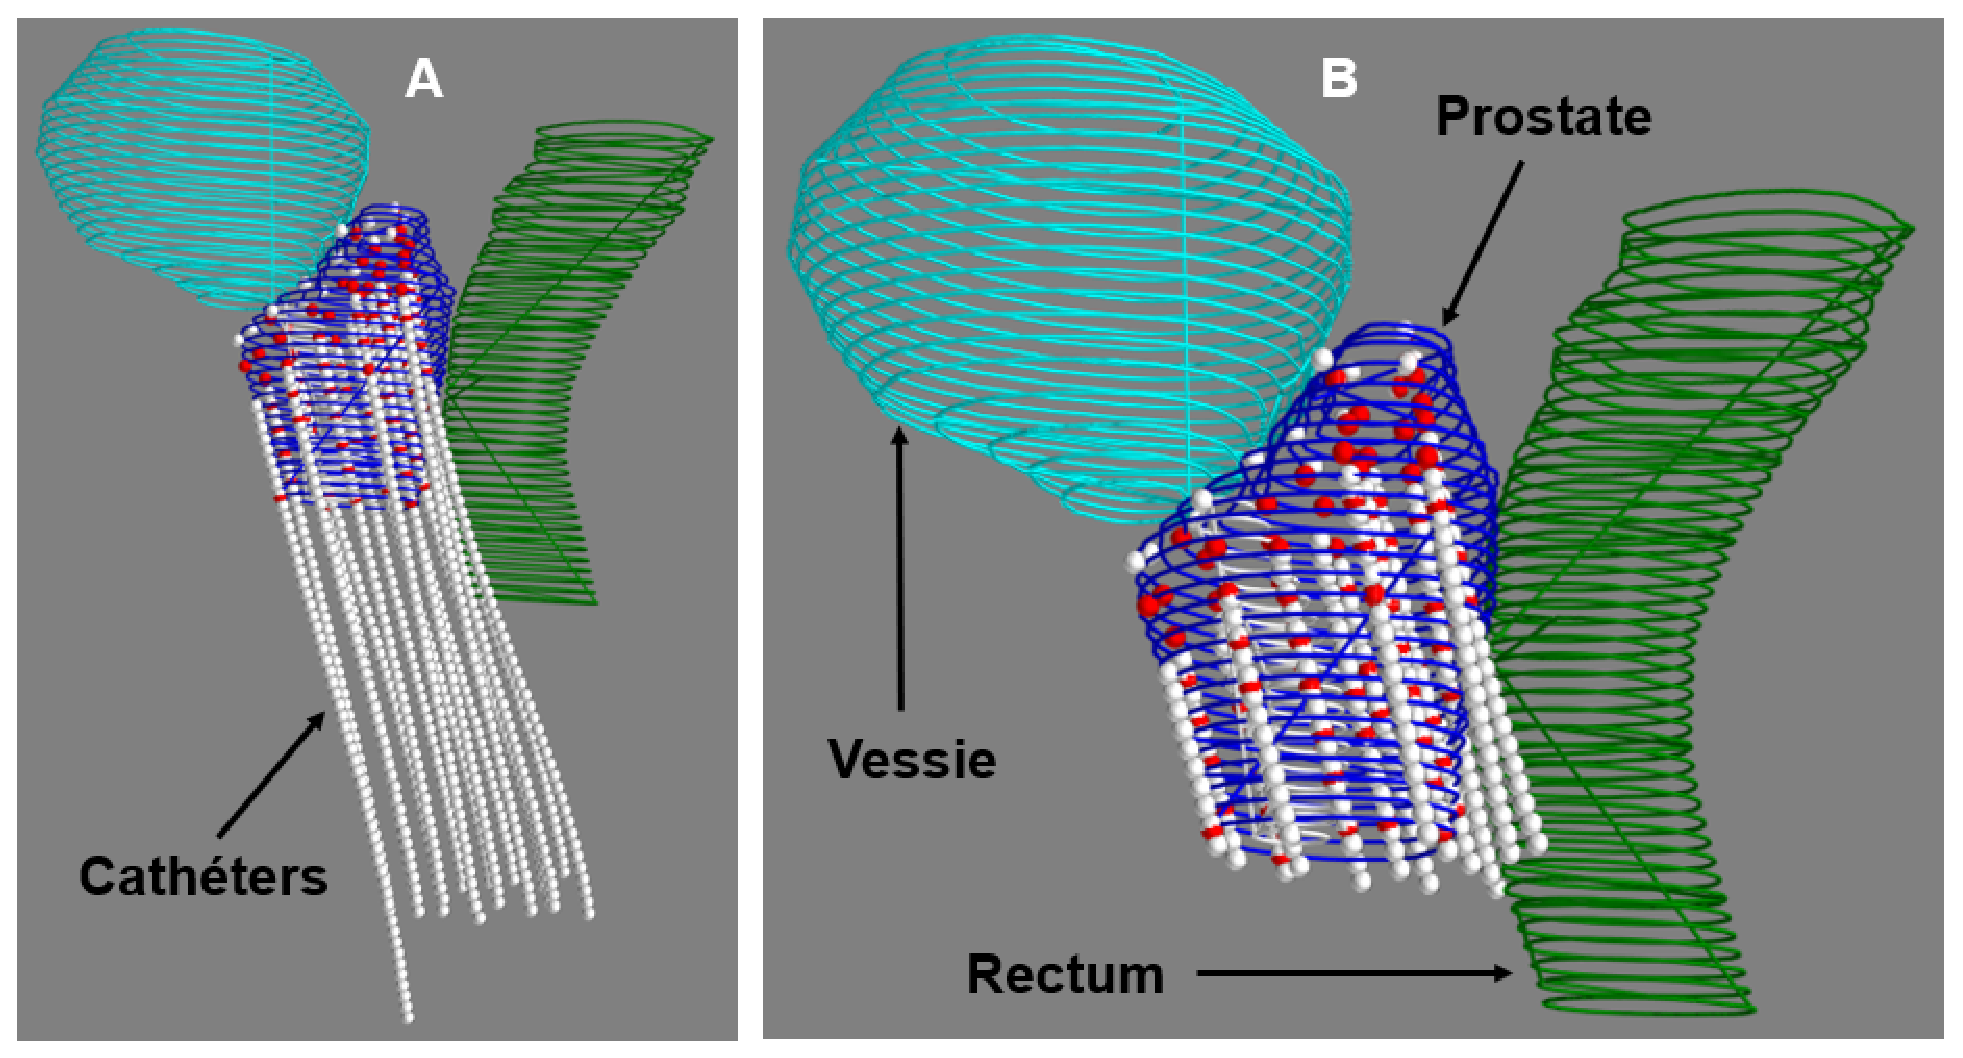
\includegraphics[width=10.5cm,height=5.8cm]{Catheters}
\caption{\label{Catheters} Illustration du processus d'évaluation de la divergence des cathéters dans le volume cible.}
\end{figure}
%
\subsection{Paramètres dosimétriques d'intérêt}
Les paramètres dosimétriques impliqués dans le processus de modélisation sont ceux qui guident le processus d'optimisation au cours de la planification, et qui sont recommandés soit par le RTOG 0924 \cite{RTOG} ou l'ABS \cite{ABS} et qui présentent une certaine variabilité inter-patients. Ces paramètres sont résumés dans le tableau \ref{IndicesDosim} ci-dessous.
%
\begin {table*}[!ht]
\captionsetup{singlelinecheck=off, skip=4pt, width =\dimexpr \textwidth-2cm\relax}%
\caption{Paramètres dosimétriques sur lesquels les modèles sont construits.}
\label{IndicesDosim} 
\renewcommand{\arraystretch}{1.4}
\vspace{-0.2cm}
\begin{center}
\begin{tabular}{llrrrrrrrrrrrr}
\toprule[1.3pt]
\hline
\multicolumn{1}{l} \textbf{Structures d'intérêts} & {} & {} & {} & {} & \multicolumn{5}{c} \textbf{Indices dosimétriques} & {} & {} \\
\cline{3-13}
\multicolumn{1}{c}{\scriptsize \textbf{}} & {} & V$_{130}$ & {} &  V$_{125}$ & {} &  V$_{100}$ & {} &  V$_{75}$ & {} &  D$_{10}$ & {} & {} \\
\hline
 \textbf{CTV} & {} & {} & {} & {} & {} & x & {} & {} & {} & {} & {} \\
\vspace{0.1cm}
%
\textbf{Vessie} & {} &  {} & {} & {} & {} &  {} & {} & x & {} & {} & {} \\
% 
\textbf{Rectum} & {} &  {} & {} & {} & {} &  {} & {} & x & {} & {} & {} \\
%
\textbf{Urètre} & {} &  x & {} & x & {} & {} &  {} & {} & {} & x & {} \\
\bottomrule[1.3pt]
\end{tabular}
\end{center}
\end{table*}
%
Pour les indices dosimétriques présentés dans le tableau ci-dessus, V$_{x}$ désigne le pourcentage du volume recevant au moins $x$\% de la dose prescrite, tandis que D$_{x}$ est la dose reçue par un pourcentage $x$ du volume irradié. L'ABS recommande une couverture minimale du CTV de 90\%, tout en minimisant la dose aux OARs (V$_{75}$ pour la vessie et le rectum < 1 cm$^{3}$) et V$_{125}$ pour l'urètre < 1 cm$^{3}$. Un réajustement de l’implant est recommandé par cet organisme si les limites de doses aux OARs pour un plan donné ne peuvent pas être obtenues. D'autre part, V$_{130}$ (respectivement D$_{10}$) qui sont des paramètres recommandés par le RTOG 0924 devraient être maintenus en dessous de 118\% de la dose de prescription (respectivement égal à zéro). Les indices dosimétriques qui ont fait l'objet de la modélisation sont V$_{100}$, V$_{75}$ et D$_{10}$; V$_{130}$ et V$_{125}$ étant nulles pour l'échantillon considéré. L'approche dans l'automation de l'extraction de ces indices dosimétriques à partir de DVHs extraits de 3D Slicer a été la même que celle présentée dans la sous-section \ref{Parag}. La figure \ref{ModeleRegresIndice} illustre les modèles de régression obtenus pour les indices dosimétriques D$_{10}$ (normalisée à la dose de prescription) et V$_{75}$ pour le rectum.
%
\begin{figure}[ht!]
  \centering
  \subfloat{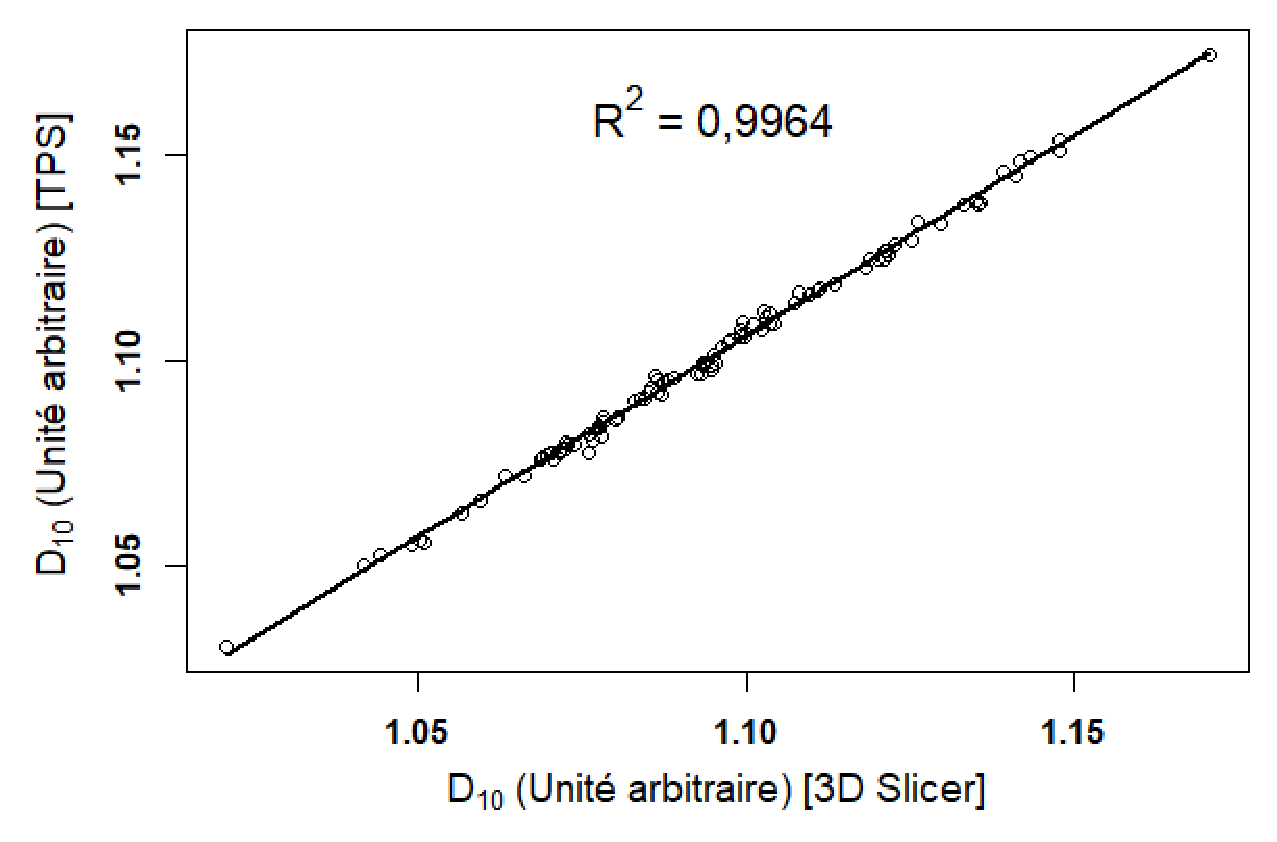
\includegraphics[width=7.2cm,height=5.2cm]{RegresD10U}\label{fig:RegresD10U}}
  \hspace{0.5cm}
  \subfloat{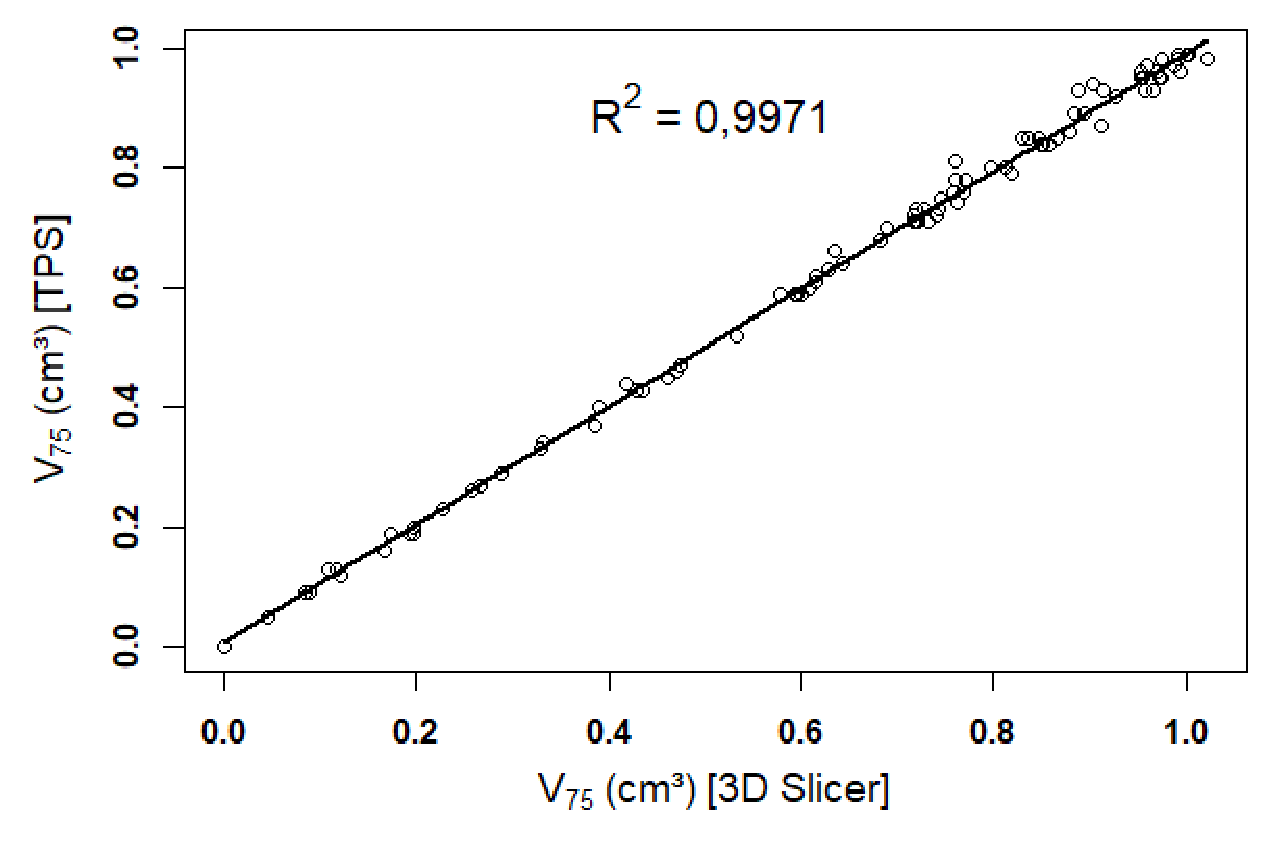
\includegraphics[width=7.2cm,height=5.2cm]{RegresV75R}\label{fig:RegresV75R}}
  \hspace{0.5cm}
\caption{\label{ModeleRegresIndice} Modèles de régression linéaire des indices dosimétriques construits à partir des DVHs extraits de 3D Slicer.}
\end{figure}
%
\section{Processus d'optimisation}
\subsection{Outil d'optimisation}
Les différentes frontières ont été optimisées avec la méthode de maximisation de la vraisemblance avec le logiciel statistique R \cite{R@2017}; le processus d'optimisation a donc consisté pour chaque modèle, à déterminer les valeurs des paramètres optimales de \enquote{c} et \enquote{$\beta$} de l'équation (\ref{eqn:Chp2Cobb2}) qui maximisent cette vraisemblance. Le logiciel R en lui-même est un logiciel de statistique gratuit et à code source ouvert (open-source). Il présente ce double avantage d'être à la fois un langage informatique (langage interprété) et un environnement de travail permettant de réaliser des analyses statistiques telles que: la statistique descriptive, les tests d’hypothèses les méthodes de régression linéaire (simple et multiple). Le logiciel R implémente plusieurs algorithmes d'optimisation, parmi lesquels, les algorithmes basés sur les gradients (Nelder-Mead ; quasi-Newton ; gradient conjugué ; BFGS quasi-Newton ; SANN) et un algorithme basé sur le recuit simulé GenSA \cite{GenSA@2012}. Les algorithmes basés sur les gradients qui sont implémentés dans la fonction \enquote{optim} dans R présentent un inconvénient majeur, leur difficulté à ne pas être piégés dans les minima locaux. D'autre part, la fonction \enquote{optim} n'offre pas la possibilité d'imposer des contraintes sur les paramètres à optimiser, exemple de $\sigma_{u} ≥ 0$ et $\sigma_{v} ≥ 0$. L’algorithme GenSA, du fait qu'il soit basé sur le recuit simulé, permet de traiter les problèmes plus complexes (fortement non linéaire); il est donc capable de sauter plusieurs minima locaux qui ne sont pas réellement optimaux. Il est également plus flexible du fait qu'il offre la possibilité de définir le domaine de variabilité des différents paramètres à optimiser tout en les imposant des contraintes.
%
\subsection{Principe d'optimisation par la méthode de maximisation de la vraisemblance}
La méthode du maximum de vraisemblance développée en 1922 \cite{Stigler@2007, Aldrich@1997} par le statisticien Ronald Aylmer Fisher est une méthode statistique qui, à partir d’un échantillon observé, permet d’inférer les meilleures valeurs des paramètres d'une distribution de probabilité. Le principe de la méthode repose dans la construction d’une fonction dite de vraisemblance que l’on cherche à maximiser par rapport aux paramètres de la distribution inconnus. Soient $x_{1}$, $x_{2}$, $x_{3}$,…, $x_{n}$, $n$ observations indépendantes d’un phénomène continu \enquote{X} gouverné par une densité de probabilité $f_{\theta}$, la fonction de vraisemblance  $L(\theta)$ est donnée par l’équation (\ref{eqn:Vraisemb}),
%
\begin{equation}\label{eqn:Vraisemb}
	L (\theta) =\prod^{n}_{i=1}f\left(x_{i}, \theta\right)
\end{equation}
%
où $\theta$ est un vecteur de paramètres inconnus à déterminer au cours du processus d’optimisation. Dans la pratique, l'équation (\ref{eqn:Vraisemb}) est linéarisée pour faciliter la recherche de la solution, ce qui conduit à l'équation (\ref{eqn:Vraisemb2}),
%
\begin{equation}\label{eqn:Vraisemb2}
\mathcal{L} = \sum^{n}_{i=1}ln\left[f\left(x_{i}, \theta\right)\right]
\end{equation}
%
L'application de ce formalisme dans la recherche des paramètres optimaux d'un modèle de FS conduit à l'équation (\ref{eqn:Vraisemb3}) dans laquelle $\varphi (.)$ (respectivement $\Phi (.)$) sont la densité de probabilité d'une loi normale centrée et réduite (respectivement sa fonction de partition).
%
\begin{equation}\label{eqn:Vraisemb3}
\mathcal{L} = \sum^{n}_{i=1}ln\left(\frac{2}{\sigma}.\varphi\left(\frac{\epsilon_{i}}{\sigma}; 0; 1\right).\left[1-\Phi\left(-\epsilon_{i}\frac{\lambda}{\sigma};0;1\right)\right]\right)
\end{equation}
%
Les contraintes imposées aux paramètres des équations (\ref{eqn:Chp2Cobb2}) et (\ref{eqn:Vraisemb3}) sont telles que $\sigma_{u} ≥ 0$ et $\sigma_{v} ≥ 0$; $c$, $\beta$ et $\alpha$ des réels. Il convient cependant de souligner qu'une valeur négative du paramètre \enquote{c} n'a pas de sens physique, toutes les observations étant positives, mais le fait d'élargir le domaine de variabilité de ce paramètre dans l'ensemble des nombres réels donne assez de marge de manœuvre à l'algorithme GenSA dans la recherche des paramètres optimaux.
%
\section{Résultats des optimisations}
\subsection{Corrélation linéaire entre les paramètres géométriques et dosimétriques}
La phase de la modélisation des FS a été précédée par une recherche de corrélation linéaire simple entre chaque indice dosimétrique d'intérêt et chaque paramètre géométrique, bien qu'une telle corrélation ne soit pas nécessaire pour que ce paramètre puisse contribuer à la construction du modèle de FS associé avec une importance statistiquement significative. En effet, les modèles de FS ne correspondent pas à des ajustements, mais plutôt en la comparaison des plans de l'échantillon, chacun ayant un profil de paramètres géométrique qui lui est propre. L'ensemble des résultats montre qu'aucune corrélation linéaire claire ne peut être dégagée entre chacun des paramètres géométriques et les différents indices dosimétriques. La figure \ref{ModeleRegresPG} illustre un exemple de la qualité de la régression entre la couverture du CTV et son volume ou entre la couverture du CTV et le volume du rectum. 
%
\begin{figure}[htt!]
  \centering
  \subfloat{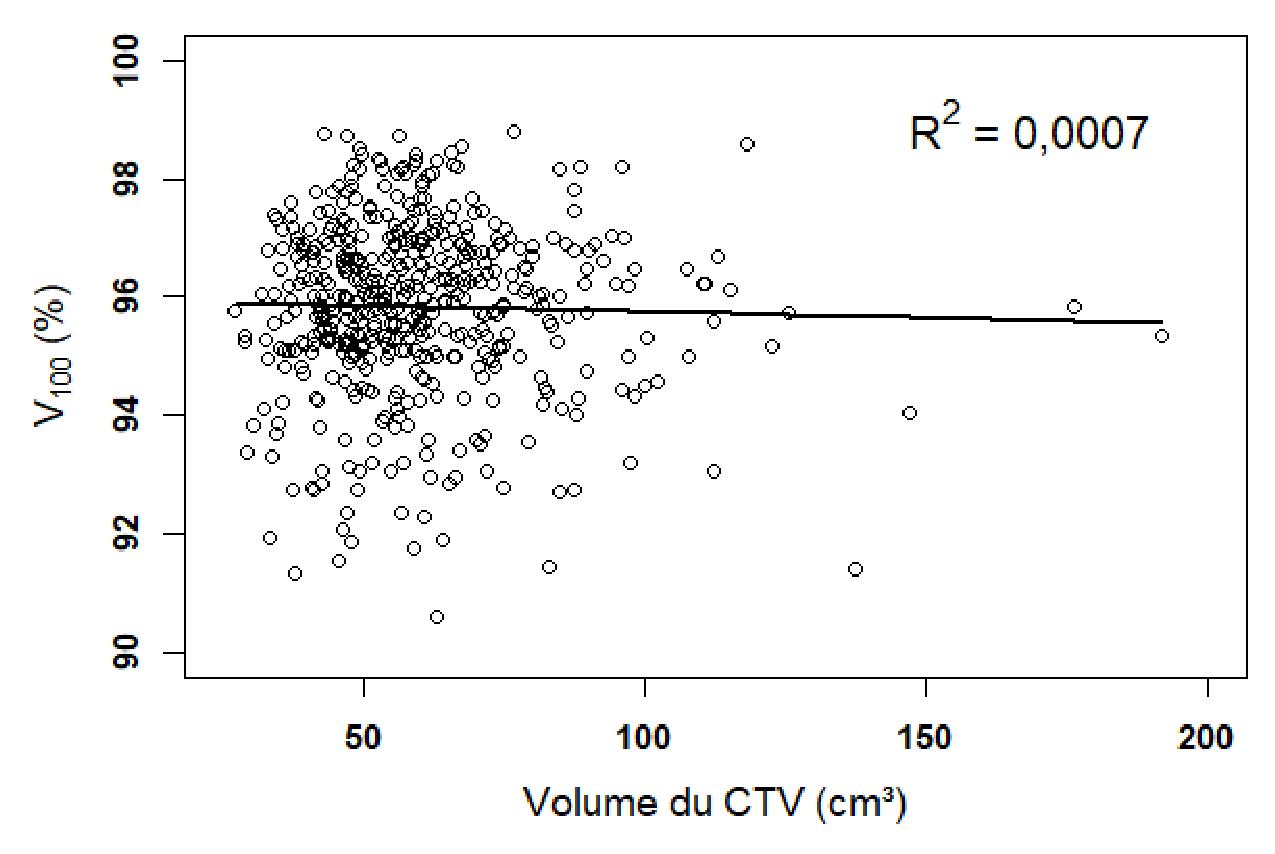
\includegraphics[width=7.2cm,height=5.2cm]{RegresV100-VolCTV}\label{fig:RegresV100-VolCTV}}
  \hspace{0.5cm}
  \subfloat{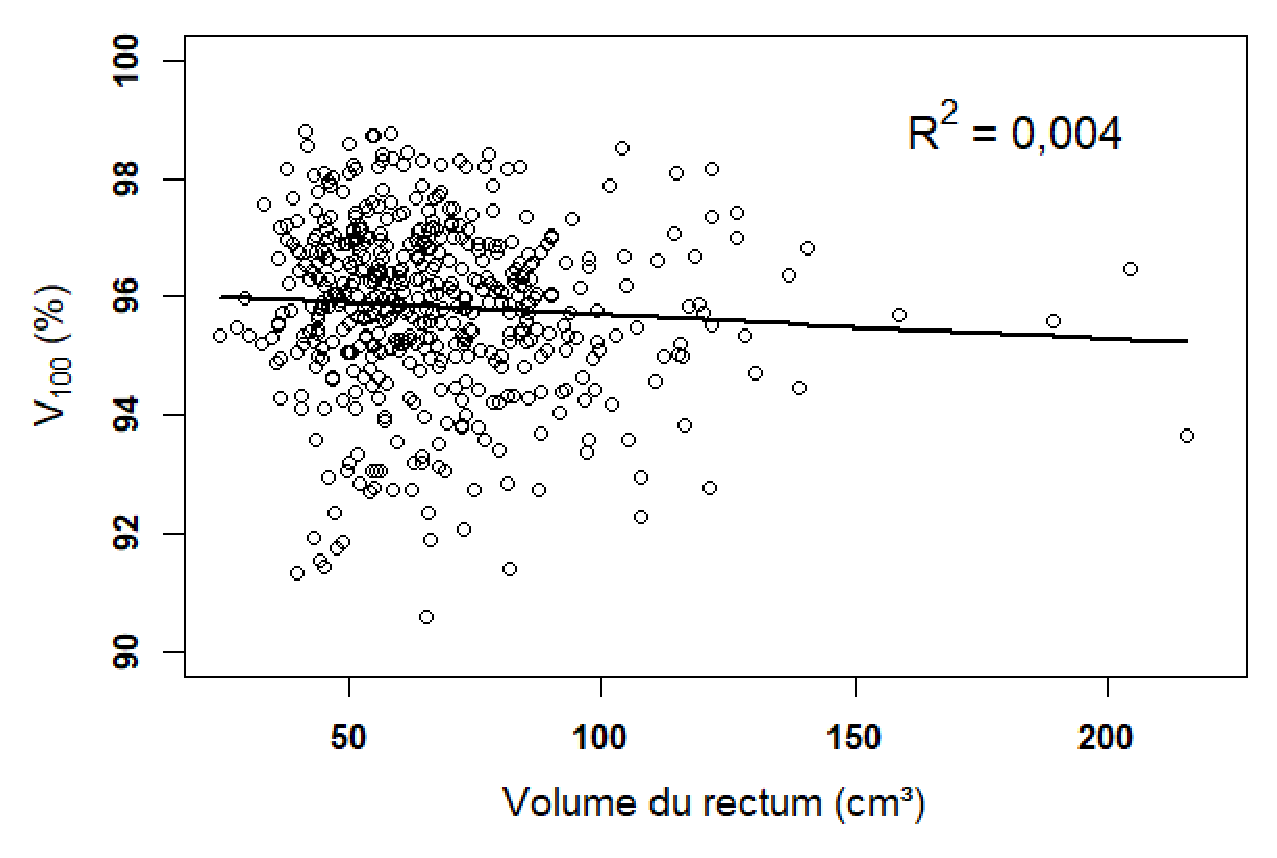
\includegraphics[width=7.2cm,height=5.2cm]{RegresV100-VolRectum}\label{fig:RegresV100-VolRectum}}
  \hspace{0.5cm}
\caption{\label{ModeleRegresPG} Modèles de régression linéaire pour la couverture du CTV en fonction du volume du CTV et le volume du rectum.}
\end{figure}
%
Le tableau \ref{coeffDeterm} résument les valeurs du coefficient détermination obtenues pour les différents modèles de régression et pour l'ensemble des paramètres géométriques.
%
\begin {table}[ht!]
\caption{Résumé de la qualité de la régression linaire simple entre chaque paramètre dosimétrique d'intérêt et les différents paramètres géométriques. Les lettres R, V et U désignent le rectum, la vessie et l'urètre, respectivement. Vol-x et Haus-x font référence, respectivement, au volume de l'organe x et à la distance de Hausdorff entre le CTV et l'organe x. P-moy est la pente moyenne des cathéters dans le CTV.}
\label{coeffDeterm} 
\renewcommand{\arraystretch}{1.4}
\begin{tabular}{llrrrrrrrrrrr}
\toprule[1.3pt]
\hline
\multicolumn{1}{l} \textbf{Modèles} & {} & {} & \multicolumn{5}{c} \textbf{Coefficient de détermination (R$^{2}$)} \\
\cline{3-10}
\multicolumn{1}{c}{\scriptsize \textbf{}} & {} & Vol-CTV & Vol-R &  Vol-V &  Vol-U & P-moy & Haus-R & Haus-V & Haus-U \\
\hline
 \textbf{V$_{100}$} & {} & 0,0007 & 0,0042 & 0,0099 & 0,0343 & 0,0012 & 0,0113 & 0,0167 & 0,0001  \\
\vspace{0.1cm}
%
\textbf{V$_{75}$ (R)} & {} & 0,0962 &  0,0063 & 0,0019 & 0,0012 & 0,0166 &  0,0 & 0,0274 & 0,0790 \\
% 
\textbf{V$_{75}$ (V)} & {} & 0,0074 &  0,0147 & 0,0060 & 0,0049 & 0,0025 & 0,0018 & 0,0207 & 0,0083  \\
%
\textbf{D$_{10}$ (U)} & {} & 0,0033 &  0,0088 & 0.0 & 0,0055 & 0,0027 & 0,0052 &  0,0141 & 0,0047 \\
\bottomrule[1.3pt]
\end{tabular}
\end{table}
%
\subsection{Modèle de FS par paramètre géométriques}
La figure \ref{ModeleFS-VolCTV} présente le résultat des modèles de FS, qualifiés de modèles de base du fait qu'ils sont optimisés avec un seul paramètre géométrique, le volume du CTV. Les plans optimaux sont ceux situés au-dessus de la frontière pour le modèle V$_{100}$ (frontière de production), et en dessous des frontières pour les autres paramètres (frontières de coût). Le modèle correspondant au paramètre V$_{75}$ pour le rectum correspond à un ajustement ($\sigma_{u} = 0$). L’interprétation de ce résultat est que l’indice dosimétrique V$_{75}$ pour le rectum est un paramètre bien optimisé en clinique, son amélioration n’est donc plus possible pour l’ensemble des plans qui constituent l’échantillon. Par contre, on observe pour les autres paramètres pour le CTV, la vessie et l’urètre, qu’un grand nombre de plans sont localisés en dessous de la frontière pour V$_{100}$, et au-dessus de la frontière pour D$_{10}$  et V$_{75}$ (vessie); ceci témoigne que ces deux paramètres dosimétriques sont améliorables pour l’échantillon considéré et peuvent être prédits pour un nouveau plan caractérisé par le volume du CTV. La figure \ref{ModeleFS-Boxplot} résume la distribution de $\epsilon$ pour V$_{100}$ et V$_{75}$ (vessie) par paramètre géométrique; les résultats sont similaires dans le cas de D$_{10}$. Les plans optimaux sont ceux pour lesquels la variable aléatoire $\epsilon$, c'est-à-dire, l'écart entre le plan optimisé par le TPS Oncentra Brachy et celui prédit par la frontière est négatif pour le CTV et positif pour la vessie et l'urètre. Cependant, ces modèles ayant comme seul paramètre géométrique, le volume du CTV, ne sont pas représentatifs de la réalité, étant donné que la couverture de la prostate est influencée par d’autres paramètres géométriques, notamment: les volumes des autres structures et leur proximité mutuelle par rapport au CTV, d'où l'intérêt de les combiner linéairement dans un modèle global.
%
\begin{figure}%[ht!]
  \centering
  \subfloat{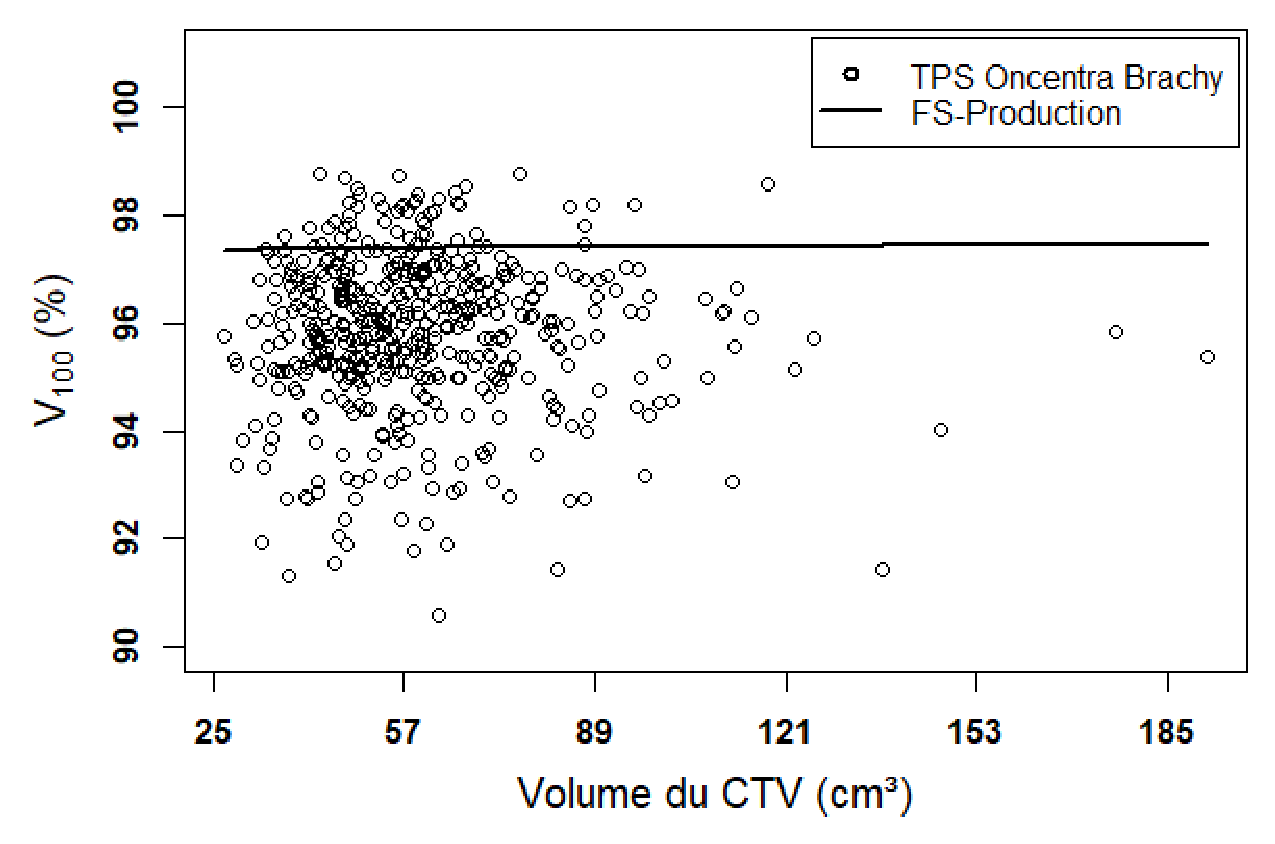
\includegraphics[width=7.2cm,height=5.2cm]{FSV100-CTV}\label{fig:FSV100-CTV}}
  \hspace{0.5cm}
  \subfloat{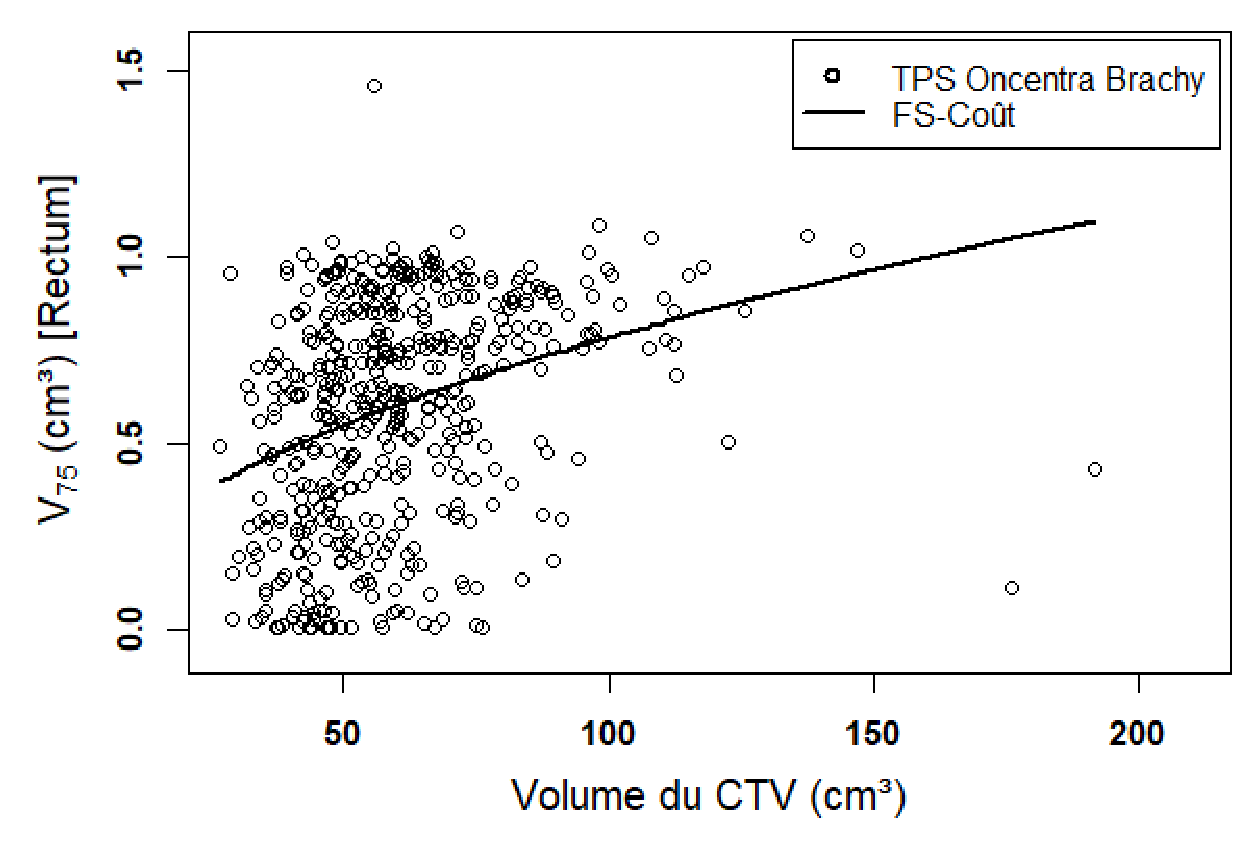
\includegraphics[width=7.2cm,height=5.2cm]{FSV75R-CTV}\label{fig:FSV75R-CTV}}
  \hspace{0.5cm}
  \subfloat{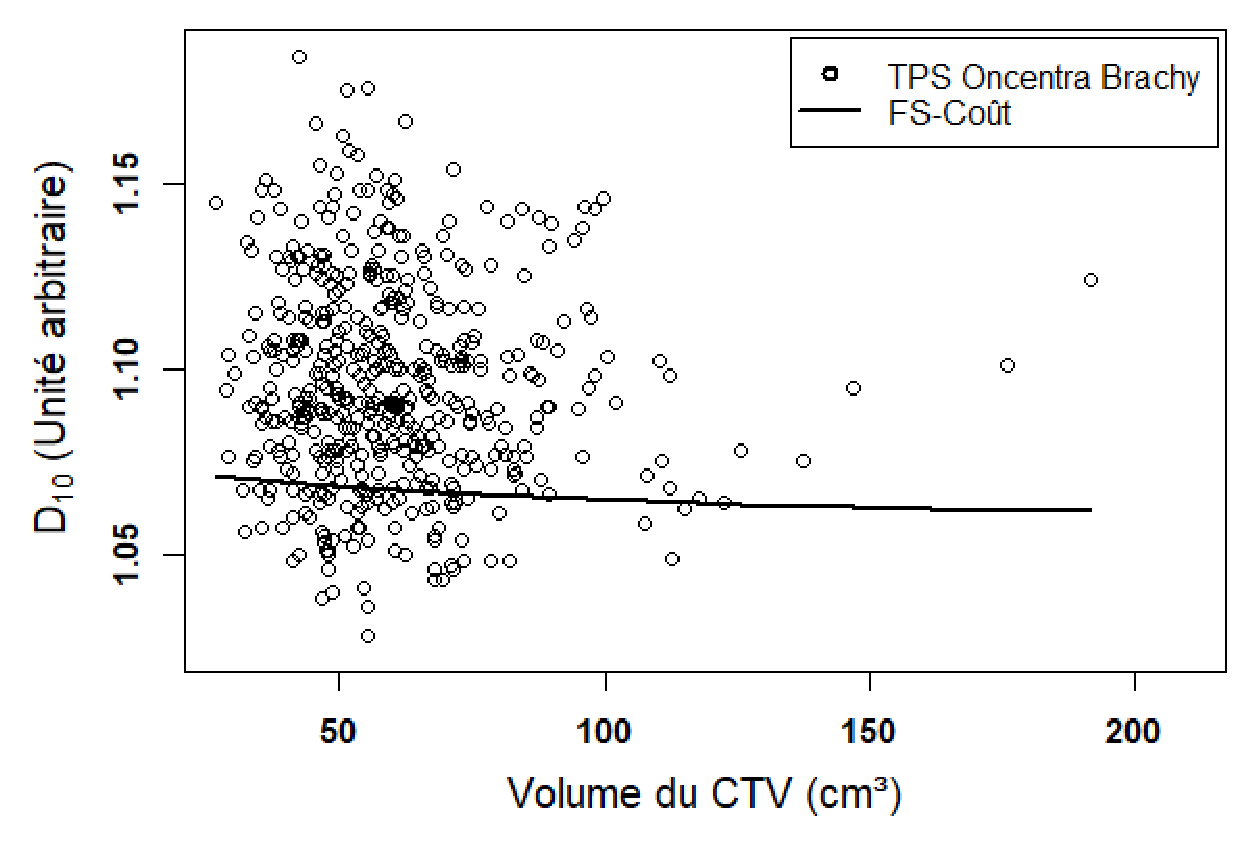
\includegraphics[width=7.2cm,height=5.2cm]{FSD10U-CTV}\label{fig:FSD10U-CTV}}
  \hspace{0.5cm}
  \subfloat{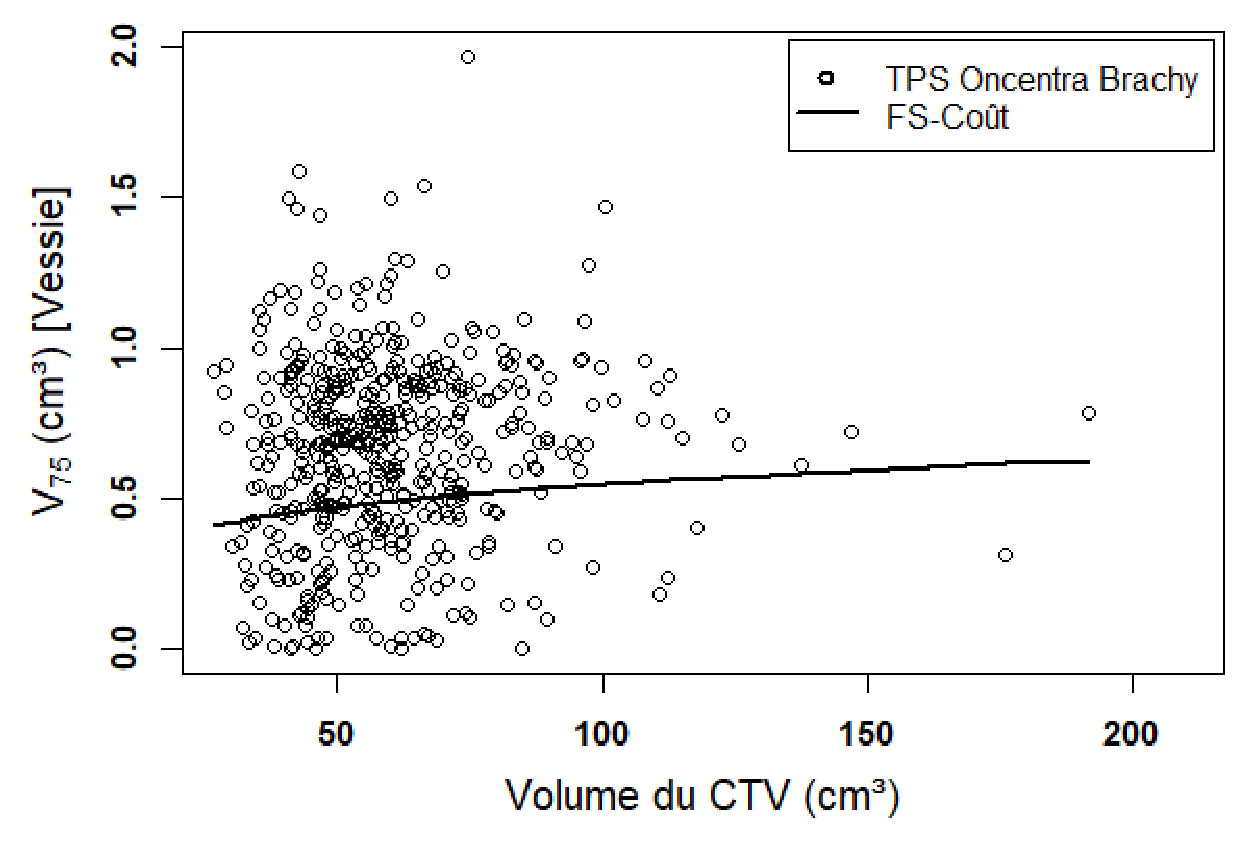
\includegraphics[width=7.2cm,height=5.2cm]{FSV75V-CTV}\label{fig:FSV75V-CTV}}
\caption{\label{ModeleFS-VolCTV} Modèles FS optimisés avec le volume du CTV pour chaque paramètre dosimétrique d'intérêt.}
\end{figure}
%
\begin{figure}[ht!]
  \centering
  \subfloat{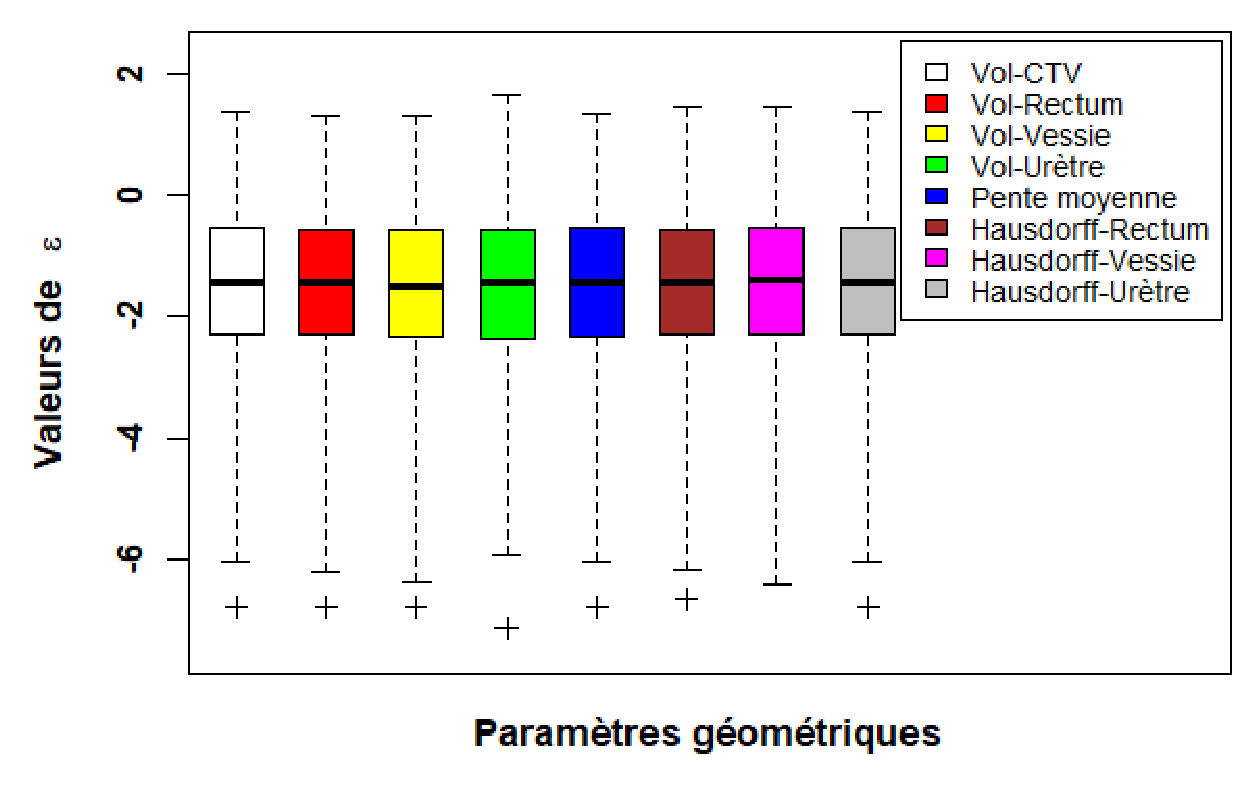
\includegraphics[width=7.2cm,height=5.2cm]{BoxplotCTV}\label{fig:BoxplotCTV}}
  \hspace{0.5cm}
  \subfloat{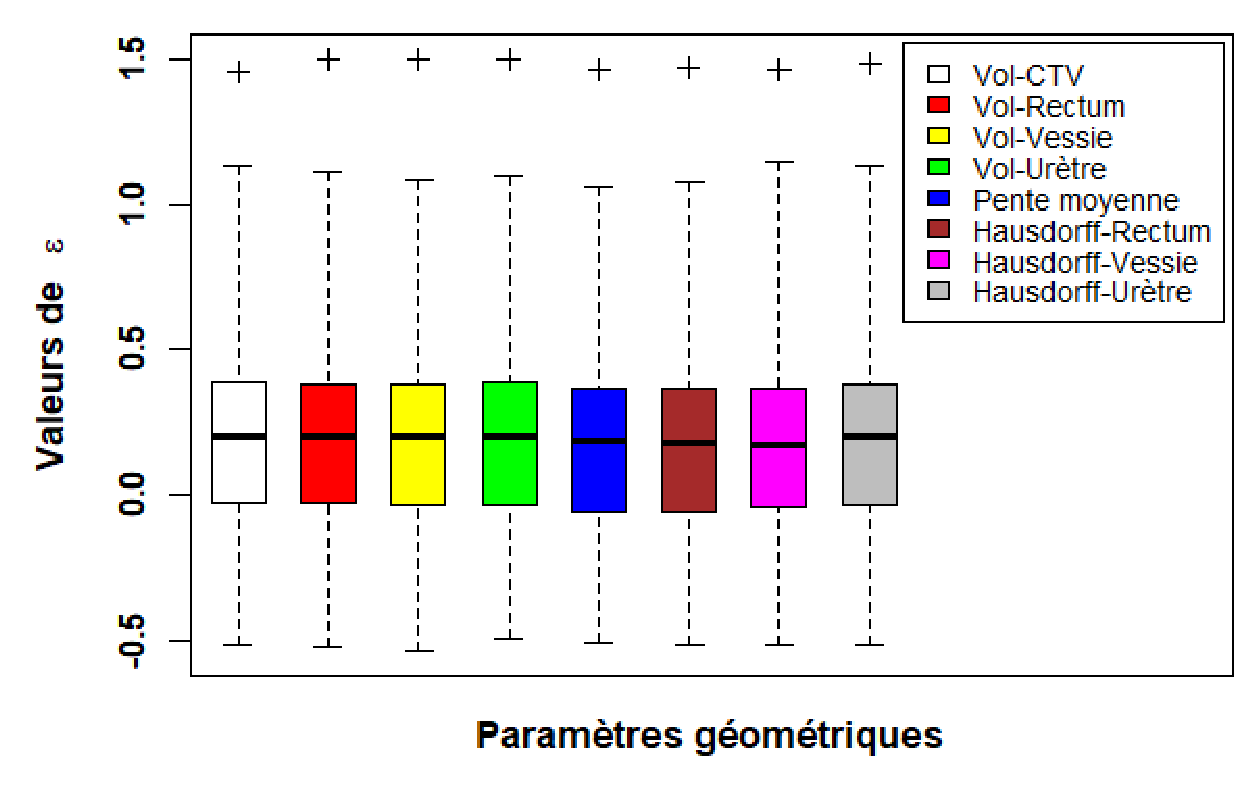
\includegraphics[width=7.2cm,height=5.2cm]{BoxplotV}\label{fig:BoxplotV}}
\caption{\label{ModeleFS-Boxplot} Distribution de $\epsilon$ pour la couverture du CTV (V$_{100}$) et l'indice dosimétrique V$_{75}$ (vessie) en fonction de chaque paramètre géométrique.}
\end{figure}
%
Les valeurs négatives de $\epsilon$ dans la figure \ref{ModeleFS-Boxplot} représentent les plans non optimaux situés en dessous de la FS de production (V$_{100}$), tandis que les valeurs positives de la même variable représentent les plans non optimaux qui sont localisés au-dessus des FS de coût (V$_{75}$, D$_{10}$).
%
\subsection{Modèle de FS complet} \label{subsec:Comb.Lineaire}
\subsubsection{Combinaison linaire des paramètres géométriques}
La construction du modèle global s’est faite en combinant tous les paramètres géométriques selon l’équation \ref{eqn:Chp2Cobb2}.  L’ajout d’un paramètre au modèle fait évoluer la vraisemblance et le test de ratio de vraisemblance donnée par l’équation \ref{eqn:P-value} a été utilisé pour statuer si la variation observée de la vraisemblance suite à l’ajout d’un nouveau paramètre géométrique est statistiquement significative à un seuil de 5\%. La valeur p (p-value) ainsi calculée a permis de déterminer si le modèle à $n$ paramètres est amélioré par rapport à celui de $n-1$ paramètres.
%
\begin{equation}\label{eqn:P-value}
LRT = -2ln\left[\frac{L_{s\left(\theta\right)}}{L_{g}\left(\theta\right)}\right]
\end{equation}
%
$L_{s\left(\theta\right)}$ et $L_{s\left(\theta\right)}$ sont respectivement la valeur de la vraisemblance pour le modèle simple (s, $n-1$ paramètres) et le modèle généralisé (g, $n$ paramètres). La distribution de probabilité du LRT (likelihood ratio test) \nomenclature{LRT}{Likelihood Ratio Test} est gouvernée par une loi du $\chi^{2}$ dont le nombre de degrés de liberté correspond à la différence entre le nombre de paramètres géométriques des deux modèles. La p-value exprimant le risque limite pour lequel on passe de l'hypothèse H$_{0}$ acceptée (le paramète ajouté améliore le modèle) à H$_{0}$ refusée, peut ainsi être calculée avec la fonction de répartition de la loi du $\chi^{2}$ \cite{P-value1,p-value2}. Les tableaux (\ref{ResumeparaFSV100} - \ref{ResumeparaFSD10}) ci-dessous résument les résultats obtenus pour ($\sigma_{u}, \sigma_{v}$), la p-value et $\mathcal{L}$ pour les trois FS (V$_{100}$, V$_{75}$ (vessie) et D$_{10}$ ). La p-value a été calculée en comparant la vraisemblance du modèle à $n$ paramètre par rapport à celui à $n-1$ paramètres (équation \ref{eqn:P-value}). 
%
\begin {table}[ht!]
\captionsetup{singlelinecheck=off, skip=4pt, width =\dimexpr \textwidth-2.5cm\relax}%
 \centering
\caption{Évolution de ($\sigma_{u}, \sigma_{v}$), la p-value et $\mathcal{L}$ en fonction du nombre de paramètres géométriques pour la couverture du CTV. Le modèle de base est constitué du volume du CTV comme paramètre géométrique.}
\label{ResumeparaFSV100}
\vspace{0.2cm}
\renewcommand{\arraystretch}{1.4}
\begin{tabular}{clrrrrrrrrrrr}
\toprule[1.3pt]
\hline
\multicolumn{1}{l} \textbf{Nombre de paramètres} & {} & \multicolumn{5}{c} \textbf{Paramètres du modèle} \\
\cline{3-10}
\multicolumn{1}{c} {géométriques \color{white} es} & {} & $\sigma_{u}$ & {} & $\sigma_{v}$ & {} & p-value & {} & $\mathcal{L}$  \\
\hline
\textbf{Modèle de base} & {} & 1,9887 & {} & 0,8252 & {} & - & {} & 874,302 &  \\
\vspace{0.1cm}
%
\textbf{2} & {} & 1,9875 &  {} & 0,8200 & {} & \textbf{0,0902} & {} & 872,867  \\
% 
\textbf{3} & {} & 1,9970 &  {} & 0,8006 & {} & 0,0159 & {} & 869,962   \\
%
\textbf{4} & {} & 1,9713 &  {} & 0,7787 & {} & 0.0 & {} & 860,949  \\
%
\textbf{5} & {} & 1,9700 &  {} & 0,7765 & {} & \textbf{0,2382} & {} & 860,253  \\
%
\textbf{6} & {} & 1,9592 &  {} & 0,7822 & {} & \textbf{ {\color{red} 0.3452}} & {} & 859,807  \\
%
\textbf{7} & {} & 1,9423 &  {} & 0,7692 & {} & 0,0007 & {} & 854,062  \\
%
\textbf{8} & {} & 1,9504 &  {} & 0,7551 & {} & 0,0492 & {} & 852,129  \\
\bottomrule[1.3pt]
\end{tabular}
\end{table}
%
Les autres paramètres géométriques sont ajoutés au modèle de base dans cet ordre: Vol-rectum, Vol-vessie, Vol-urètre, P-moyenne et Hausdorff CTV-(R, V, U). Vol-x désigne le volume de la structure $x$, P-moyenne est la pente moyenne des cathéter dans la prostate et Hausdorff CTV-(R, V, U) la distance de Hausdorff entre le CTV et le rectum (R), la vessie (V), l'urètre (U).
%
\begin {table}[ht!]
\captionsetup{singlelinecheck=off, skip=4pt, width =\dimexpr \textwidth-3cm\relax}%
 \centering
\caption{Évolution de ($\sigma_{u}, \sigma_{v}$), la p-value et $\mathcal{L}$ en fonction du nombre de paramètres géométriques pour le modèle V$_{75}$ (vessie). Le modèle de base est constitué du volume du CTV comme paramètre géométrique.}
\label{ResumeparaFSV75V}
\vspace{0.2cm}
\renewcommand{\arraystretch}{1.4}
\begin{tabular}{clrrrrrrrrrrr}
\toprule[1.3pt]
\hline
\multicolumn{1}{l} \textbf{Nombre de paramètres} & {} & \multicolumn{5}{c} \textbf{Paramètres du modèle} \\
\cline{3-9}
\multicolumn{1}{c} {géométriques \color{white} es} & {} & $\sigma_{u}$ & {} & $\sigma_{v}$ & {} & p-value & {} & $\mathcal{L}$  \\
\hline
\textbf{Modèle de base} & {} & 0,2176 & {} & 0,2810 & {} & - & {} & 122,593 \\
\vspace{0.1cm}
%
\textbf{2} & {} & 0,2279 &  {} & 0,2764 & {} & 0,0026 & {} & 120,106  \\
% 
\textbf{3} & {} & 0,2316 &  {} & 0,2743 & {} & \textbf{0,0959} & {} & 118,719   \\
%
\textbf{4} & {} & 0,2898  &  {} & 0,2504 & {} & 0,0004 & {} & 112,422  \\
%
\textbf{5} & {} & 0,2533 &  {} & 0,2624 & {} & \textbf{0,1752} & {} & 111,504  \\
%
\textbf{6} & {} & 0,2562 &  {} & 0,2610 & {} & \textbf{{\color{red} 0,6517}} & {} & 111,402  \\
%
\textbf{7} & {} & 0,3094 &  {} & 0,2396 & {} & 0,0062 & {} & 107,655  \\
%
\textbf{8} & {} & 0,2783 &  {} & 0,2466 & {} & 0,0520 & {} & 105,767  \\
\bottomrule[1.3pt]
\end{tabular}
\end{table}
%
\begin {table}[ht!]
\captionsetup{singlelinecheck=off, skip=4pt, width =\dimexpr \textwidth-2.8cm\relax}%
 \centering
\caption{Évolution de ($\sigma_{u}, \sigma_{v}$), la p-value et $\mathcal{L}$ en fonction du nombre de paramètres géométriques pour le modèle D$_{10}$. Le modèle de base est constitué du volume du CTV comme paramètre géométrique.}
\label{ResumeparaFSD10}
\vspace{0.2cm}
\renewcommand{\arraystretch}{1.4}
\begin{tabular}{clrrrrrrrrrrr}
\toprule[1.3pt]
\hline
\multicolumn{1}{l} \textbf{Nombre de paramètres} & {} & \multicolumn{5}{c} \textbf{Paramètres du modèle} \\
\cline{3-9}
\multicolumn{1}{c} {géométriques \color{white} es} & {} & $\sigma_{u}$ & {} & $\sigma_{v}$ & {} & p-value & {} & $\mathcal{L}$  \\
\hline
\textbf{Modèle de base} & {} & 0,0358 & {} & 0,0177 & {} & - & {} & -1077,419 \\
\vspace{0.1cm}
%
\textbf{2} & {} & 0,0356 &  {} & 0,0177 & {} & \textbf{0.1282} & {} & -1078,577  \\
% 
\textbf{3} & {} & 0,0357 &  {} & 0,0177 & {} & \textbf{\color{red} 0,8212} & {} & -1078,602   \\
%
\textbf{4} & {} & 0,0356 &  {} & 0,0176 & {} & \textbf{0,0574} & {} & -1080,407  \\
%
\textbf{5} & {} & 0,0356 &  {} & 0,0176 & {} & \textbf{\color{red} 0,7745} & {} & -1080,448  \\
%
\textbf{6} & {} & 0,0359 &  {} & 0,0173 & {} & \textbf{0,1177} & {} & -1081,672  \\
%
\textbf{7} & {} & 0,0344 &  {} & 0,0179 & {} & 0,0131 & {} & -1084,750  \\
%
\textbf{8} & {} & 0,0340 &  {} & 0,0182 & {} & \textbf{0.3360} & {} & -1085,213  \\
\bottomrule[1.3pt]
\end{tabular}
\end{table}
%
Les paramètres géométriques pour lesquels les p-value résumés dans les tableaux (\ref{ResumeparaFSV100} - \ref{ResumeparaFSD10}) ont une valeur assez différente de la valeur critique de 5\% généralement utilisée dans la littérature ont été supprimées du modèle global; Il s’agit des valeurs mises en évidence en rouge. Les valeurs en gras dans les mêmes tableaux quant à eux, ont été conservées du fait qu’ils sont relativement proches de la valeur critique; le choix de les conserver reste cependant suggestif.\\
Bien que le modèle V$_{75}$ associé au rectum ne présente aucune efficience technique ($\sigma_{u} = 0$), la signifiance statistique de l’ajout de paramètres géométriques supplémentaires au modèle de base a été évaluée quantitativement par la même approche que celle présentée ci-dessus pour les modèles V$_{100}$, V$_{75}$ vessie et D$_{10}$; les résultats sont résumés dans le tableau \ref{ResumeparaFSV75R}. Ces résultats montrent que seuls deux paramètres géométriques (Vol-rectum, Vol-Vessie) semblent ne pas contribuer de façon significative à l’amélioration du modèle, mais tous les paramètres géométriques ont été conservés dans le modèle global, du fait des valeurs de $\sigma_{u} \approx 0$ et $\sigma_{v}$ qui sont relativement constantes quel que soit la p-value. D’autre part, le modèle ne pouvant être utilisé sur le plan prédictif, il n’y a aucun enjeu sur le choix de conserver ou de supprimer les paramètres géométriques ayant une p-value largement supérieure à la valeur critique de 5\%.
%
\begin {table}[ht!]
\captionsetup{singlelinecheck=off, skip=4pt, width =\dimexpr \textwidth-3cm\relax}%
\centering
\caption{Évolution de ($\sigma_{u}, \sigma_{v}$), la p-value et $\mathcal{L}$ en fonction du nombre de paramètres géométriques pour le modèle V$_{75}$ (rectum). Le modèle de bas est constitué du volume du CTV comme paramètre géométrique.}
\label{ResumeparaFSV75R}
\vspace{0.2cm}
\renewcommand{\arraystretch}{1.4}
\begin{tabular}{clrrrrrrrrrrr}
\toprule[1.3pt]
\hline
\multicolumn{1}{l} \textbf{Nombre de paramètres} & {} & \multicolumn{5}{c} \textbf{Paramètres du modèle} \\
\cline{3-9}
\multicolumn{1}{c} {géométriques \color{white} es} & {} & $\sigma_{u}$ & {} & $\sigma_{v}$ & {} & p-value & {} & $\mathcal{L}$  \\
\hline
\textbf{Modèle de base} & {} & 0,0 & {} & 0,2845 & {} & - & {} & 80,165 \\
\vspace{0.1cm}
%
\textbf{2} & {} & 0,0 &  {} & 0,2845 & {} & \textbf{0,9278} & {} & 80,161  \\
% 
\textbf{3} & {} & 0,0 &  {} & 0,2845 & {} & \textbf{0,8215} & {} & 80,135  \\
%
\textbf{4} & {} & 0,0140 &  {} & 0,2824 & {} & 0,0004 & {} & 73,898  \\
%
\textbf{5} & {} & 0,0 &  {} & 0,2799 & {} & \textbf{0,0658} & {} & 72,206  \\
%
\textbf{6} & {} & 0,0193 &  {} & 0,2795 & {} & \textbf{0,2701} & {} & 71,598  \\
%
\textbf{7} & {} & 0,0 &  {} & 0,2744 & {} & 0.0 & {} & 61,861  \\
%
\textbf{8} & {} & 0,0 &  {} & 0,2712 {} & {} & 0,0011 & {} & 56.510 \\
\bottomrule[1.3pt]
\end{tabular}
\end{table}
%
Les valeurs de $\sigma_{u}$ assez élevées du tableau \ref{ResumeparaFSV100} par rapport au bruit aléatoire représenté par $\sigma_{v}$ montrent que, pour l'échantillon considéré, la couverture du CTV est améliorable pour un grand nombre de plans ayant un profil de paramètres géométriques semblables ou identiques, ceci témoigne la signature de la variabilité de la qualité des plans due au jugement et l’expérience du planificateur. Cette signature est moins prononcée pour le modèle de V$_{75}$ (vessie) pour lequel le bruit aléatoire et l’efficience technique sont du même ordre de grandeur ( tableau \ref{ResumeparaFSV75V}). Les résultats concernant le modèle D$_{10}$ (tableau \ref{ResumeparaFSD10}) montrent qu’il y a très peu de marge de manœuvre pour améliorer la dose à cet OAR ($\sigma_{u}$ très faible) à cause sa position dans la prostate. Pour le modèle V$_{75}$ (rectum), certains paramètres géométriques, en l’occurrence : le volume du rectum, le volume de l’urètre et la distance de Hausdorff CTV-Rectum, lorsque pris individuellement tel que présenté dans la figure \ref{ModeleRegres} pour la couverture du CTV, présentent une efficience technique non nulle; bien que celle-ci reste faible comparativement à celle obtenue pour modèle D$_{10}$ de l'urètre (ordre de grandeur 10$^{-2}$ - 10$^{-4}$). Cependant, cette efficience technique s’estompe dès lors que tous les paramètres géométriques sont pris en compte dans une combinaison linéaire pour la construction du modèle global. Ceci témoigne bien l’importance de la prise en compte de tous les paramètres géométriques qui influencent la dose dans cet OAR, en d’autres termes, le caractère prédictif des modèles peut être sous-estimé ou surestimé si les paramètres géométriques contenus dans le modèle ne sont pas assez représentatifs du profil géométrique réel de chaque plan.
%
\subsubsection{Modèles complets}
Chaque modèle complet a pour argument (intrants), la combinaison linéaire des paramètres géométriques jugés statistiquement significatifs sur la base de l'analyse présentée dans la sous-section \ref{subsec:Comb.Lineaire}, et le tableau \ref{GWeight} résume les valeurs des poids des paramètres géométriques $\beta{i}$ de l'équation \ref{eqn:Chp2Cobb2}.
%
\begin {table}[ht!]
\captionsetup{singlelinecheck=off, skip=4pt, width =\dimexpr \textwidth-6.3cm\relax}%
\centering
\caption{Valeurs numériques des paramètres de l'équation \eqref{eqn:Chp2Cobb2} pour les différents modèles, suivies de la statistique de $\epsilon$.}
\label{FrontierNumericalValues} 
\vspace{0.1cm}
\renewcommand{\arraystretch}{1.4}
    \begin{tabular}{crrrrrrrrrrrr}
	\toprule[1.3pt]
	\hline
        Modèles optimisés               &  c     & $\alpha$  & E$(\epsilon)$ & SD \\ 
        \hline
        V$_{100}$ (\%)       & 99,219 & -0,010 & -1,556 &  1,397  \\ 
		V$_{75}$ (B)   		 & 0,122  &  0,304   &  0,169   &   0,300  \\ 
		V$_{75}$ (R)         & 0,867  &   0,489   &  0,0   &   0,271  \\ 
		D$_{10}$ (U)         & 1,216  & -0,023    &  0,027   &   0,027 \\ 
        \bottomrule[1.3pt]
	\end{tabular} 
\end {table}
%
La densité de probabilité de $\epsilon$, dont la statistique est présentée dans le tableau \ref{FrontierNumericalValues} est illustrée dans la figure \ref{DensiteProba} pour le couverture du CTV (V$_{100}$) et la limitation de la dose à l'urètre (D$_{10}$).
%
%\vspace{-0.445cm}
\begin{figure}[ht!]
  \centering
  \subfloat[(Modèle-Couverture du CTV: V$_{100}$)]{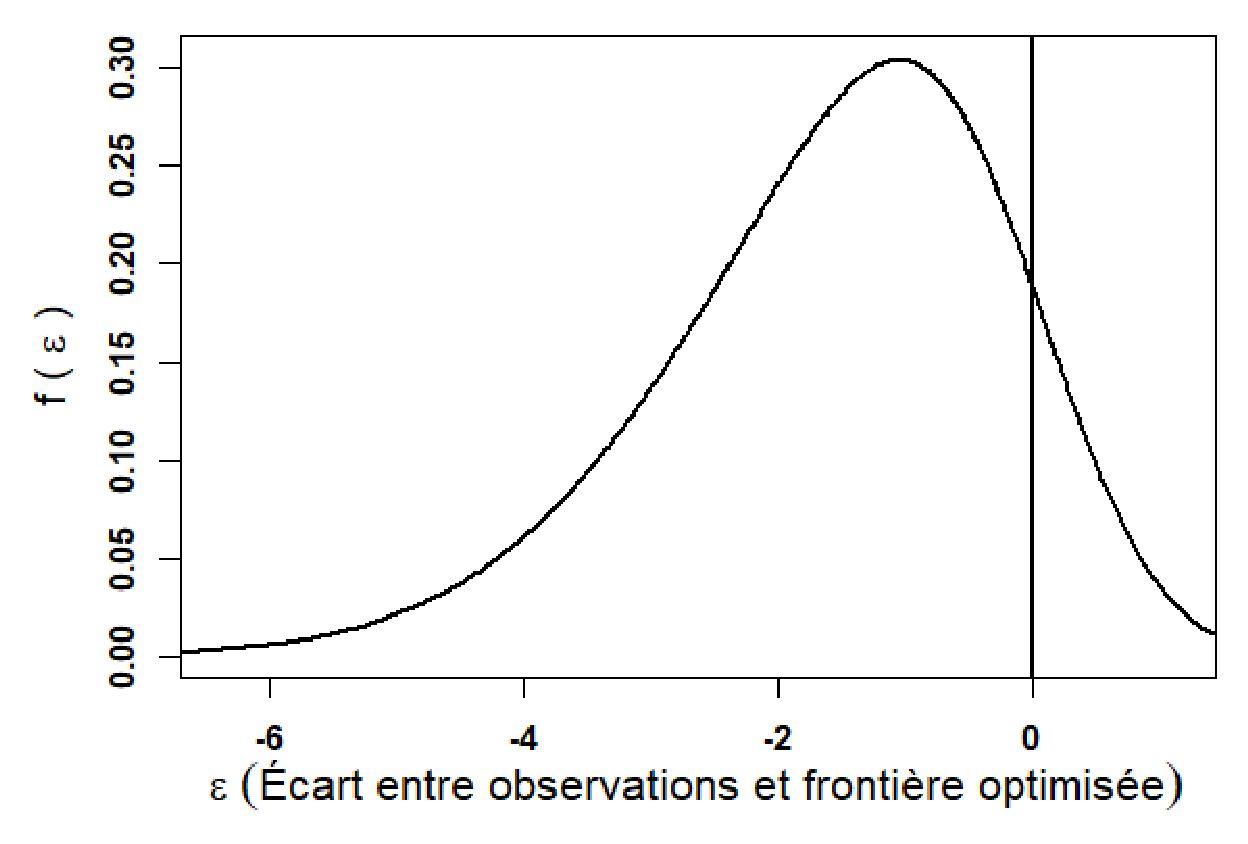
\includegraphics[width=7.2cm,height=5.2cm]{DensiteProba-CTV}\label{fig:DensiteProba-CTV}}
  \hspace{0.5cm}
  \subfloat[(Modèle-Urètre: D$_{10}$)]{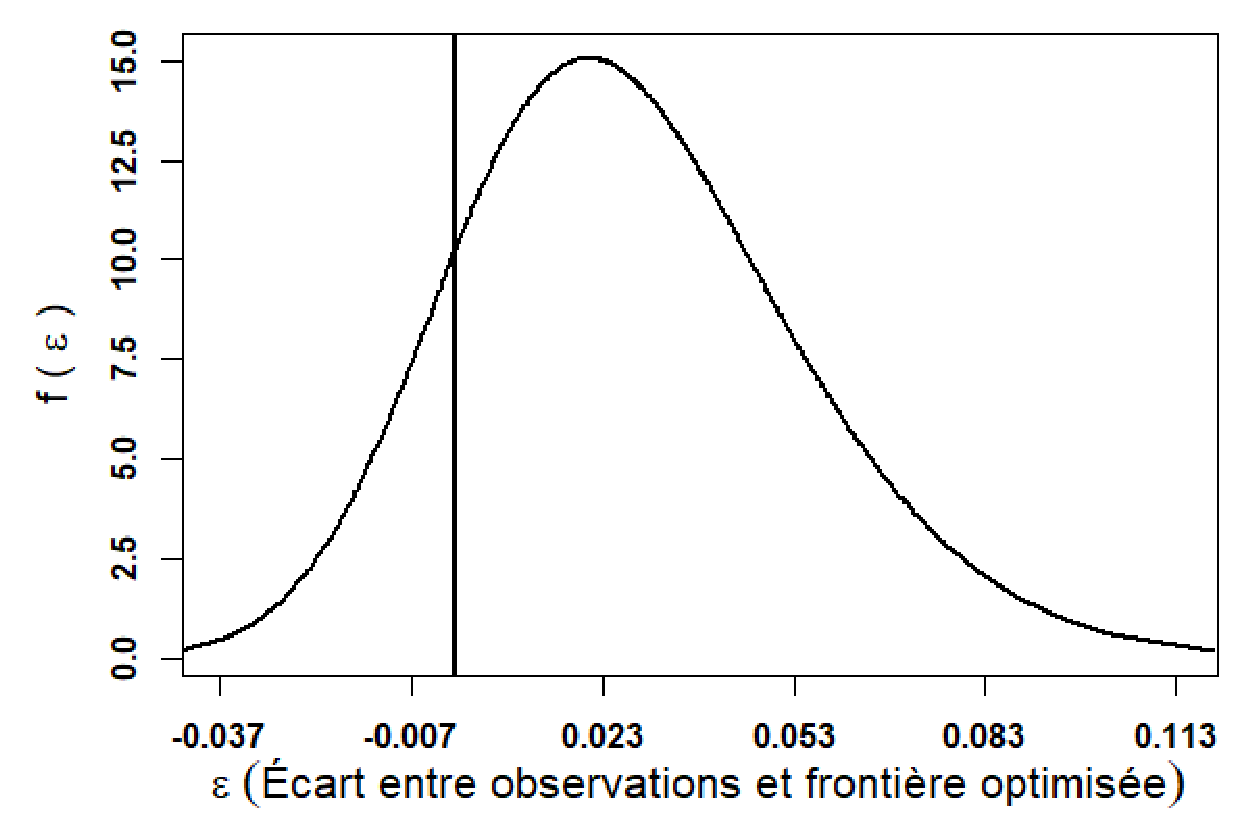
\includegraphics[width=7.2cm,height=5.2cm]{DensiteProba-D10}\label{fig:DensiteProba-D10}}
\caption{\label{DensiteProba} Illustration de la densité de probabilité moyenne relative à la combinaison linéaire des paramètres géométriques pour le modèle correspondant à la couverture du CTV (a) et à la limitation de la dose à l'urètre (b).}
\end{figure}
%
La statistique de $\epsilon$ présentée dans le tableau (\ref{FrontierNumericalValues}) et la distribution de sa densité de probabilité que l'on visualise dans figure \ref{DensiteProba} pour le modèle V$_{100}$ (respectivement D$_{10}$) sont porteurs de quelques informations. En effet, comme attendu, les deux distributions sont tronquées négatives pour V$_{100}$ (respectivement positive pour D$_{10}$) avec les domaines de variabilité compléments différents, à savoir [-6,731; 1.428] (respectivement [-0,045; 0,119]). Ces résultats montrent qu'une amélioration importante ($\epsilon$ assez grand) de la couverture du CTV est possible, comparativement aux résultats de l'urètre. La dispersion élevée autour de la moyenne E ($\epsilon$)  pour le modèle V$_{100}$, comparativement au modèle de l'urètre D$_{10}$ montre la non-uniformité de la qualité des plans pour l'échantillon considéré. Cette dispersion contient une composante liée au jugement et à l'expérience du planificateur, composante qui peut être améliorée pour de nouveaux plans par l'information prédictive contenue dans les modèles. Une analyse similaire peut être menée pour le modèle V$_{75}$ (vessie), mais la statistique de $\epsilon$ présentée dans le tableau \ref{FrontierNumericalValues} montre qu’une amélioration de ce paramètre dosimétrique est possible pour l’échantillon considéré avec une amplitude moindre et peu de variabilité inter-plan en comparaison au cas du modèle associé à la couverture du CTV (V$_{75}$, $\epsilon \in$ [-0,631; 1,493]), mais assez importante en comparaison au modèle associé à la limitation de la dose à l’urètre, D$_{10}$. Les résultats finaux pour les quatre modèles sont illustrés graphiquement dans la figure \ref{ModelGlobalFS} avec les bornes inférieures (Inf.) et supérieures (Sup.) des intervalles de confiances (IC) calculés à 95\% par la méthode Bootstrap avec 4000 Rééchantillonnages. 
%
\begin{sidewaystable}[h!]
\caption{Poids des paramètres géométriques ($\beta{i}$) optimisés pour chaque modèle. Vol-x désigne le volume de la structure $x$ et Hausd-x, la distance de Hausdorff entre le CTV et l'organe $x$; où x désigne le rectum (R), la vessie (V) et l’urètre (U). Pente-moy désigne la pente moyenne des cathéters implantés dans la prostate et SD la déviation standard des deux termes d’erreur, c’est-à-dire, l’efficience technique ($\sigma_{u}$) et le bruit aléatoire ($\sigma_{v}$).  $\beta{i}$ est exprimé en $cm^{-3}$ pour les poids associés aux volumes et en cm$^{-1}$ pour ceux correspondant à la distance de Hausdorff. La pente moyenne (Pente-moy) est une grandeur sans unité.}
\label{GWeight}
\begin{center}
\vspace{-0.5cm}
\renewcommand{\arraystretch}{1.5}
\begin{tabular}{lrrrrrrrrrrrr}
\toprule[1.3pt]
\hline
\multicolumn{1}{l} \textbf{Modèles} & {} & {} & {} & \multicolumn{4}{c} \textbf{Poids des paramètres géométriques ($\beta_{i}$)} & {} & \multicolumn{3}{c} \textbf{SD}\\
\cline{3-10}
\cline{12-13} 
\multicolumn{1}{l} \textbf{optimisés} & {} & Vol-CTV & Vol-Vessie & Vol-Rectum & Vol-Urètre & Pente-moy & Hausd-V & Hausd-R & Hausd-U & {} &  $\sigma_{u}$ & $\sigma_{v}$\\
\hline
\textbf{V$_{100}$ (CTV)} & {} & -0.058 & 0.039 & 0.013 & 3.549 & -4.996 & -0.107 & 0.023 & 0.190 & {} & 1.950 & 0.755 \\
\vspace{0.1cm}
%
\textbf{V$_{75}$ (B)} & {} & 1.756 & 0.953 & 0.654 & -33.488 & -1.731 & -1.730 & - & 0.211 & {} & 0.208 & 0.273 \\
%
\textbf{V$_{75}$ (R)} & {} & 0.007 & 0.002 & 0.001 & -0.048 & 0.441 & -0.008 & -0.002 & 0.015 & {} & 0.000 & 0.271 \\
%
\textbf{D$_{10}$ (U)} & {} & -0.305 & - & -0.950 & 60.091 & - & 3.089 & -0.493 & 2.973 & {} & 0.034 & 0.018 \\
%
\bottomrule[1.3pt]
\end{tabular}
\end{center}
\end{sidewaystable}
%
\clearpage 
CLPG (combinaison linéaire des paramètres géométriques) est le profil de paramètres géométriques caractérisant chaque plan et donné par l'équation,
%
\begin{equation}\label{eqn:ProfilPG}
	\textrm{CLPG} = \sum^{n}_{i=1}\beta_{i}x_{i}
\end{equation}
%
où $n$ est le nombre de paramètres géométriques et $\beta_{i}$ le poids des paramètres géométriques $x_{i}$ résumés dans le tableau \ref{GWeight}. Pour le modèle V$_{100}$ par exemple, CLPG est explicitement donnée par l'équation (\ref{eqn:CLPG}): 
%
\begin{multline}\label{eqn:CLPG}
\textrm{CLPG (Modèle-CTV)} = -0,058.(\textbf{Vol-CTV}) + 0,013.(\textbf{Vol-Rectum}) + 0,039.(\textbf{Vol-Vessie})\\ + 3,549.(\textbf{Vol-Urètre}) - 4,996.(\textbf{Pente-moy}) + 0,023.(\textbf{Hausd-R}) - 0,107.(\textbf{Hausd-V})\\
+ 0,190.(\textbf{Hausd-U})
\end{multline}
%
De façon analogue, le profil de paramètres géométriques (CLPG) pour les autres modèles (V$_{75}$ (vessie, rectum), D$_{10}$) sont facilement déductibles à partir de l'équation (\ref{eqn:ProfilPG}) et des valeurs des poids $\beta_{i}$ résumés dans le tableau \ref{GWeight}. Rappelons que les plans optimaux sont ceux qui sont situés au-dessus de la frontière de production (V$_{100}$) et en dessous de la frontière de coût pour les OARs (V$_{75}$, D$_{10}$).  L’analyse quantitative de la figure \ref {ModelGlobalFS} révèle que la plus grande efficience technique est obtenue pour V$_{75}$ (rectum, $\sigma_{u} = 0$). Ce résultat corrobore avec les informations recueillies auprès des physiciens, selon lesquelles, le rectum est un OAR pour lequel beaucoup d’attention est accordée pour minimiser la dose au cours de la panification, parfois au détriment de la vessie. La plus faible efficience technique est observée pour la couverture du CTV, V$_{100}$. En effet, 83\% des plans sont localisés en dessous de la frontière, avec un écart maximum de 6,4\% par rapport au plan le plus distant de la frontière. En ce qui concerne la vessie (respectivement l’urètre), \textasciitilde 50\% des plans sont situés au-dessus de la frontière de V$_{75}$ avec un écart maximum de 1,28 cm$^{3}$ (respectivement \textasciitilde 72\% des plans au-dessus de la frontière D$_{10}$ avec une différence de dose maximale 1,56 Gy). 
%
\begin{figure}[htp!]
  \centering
  \subfloat{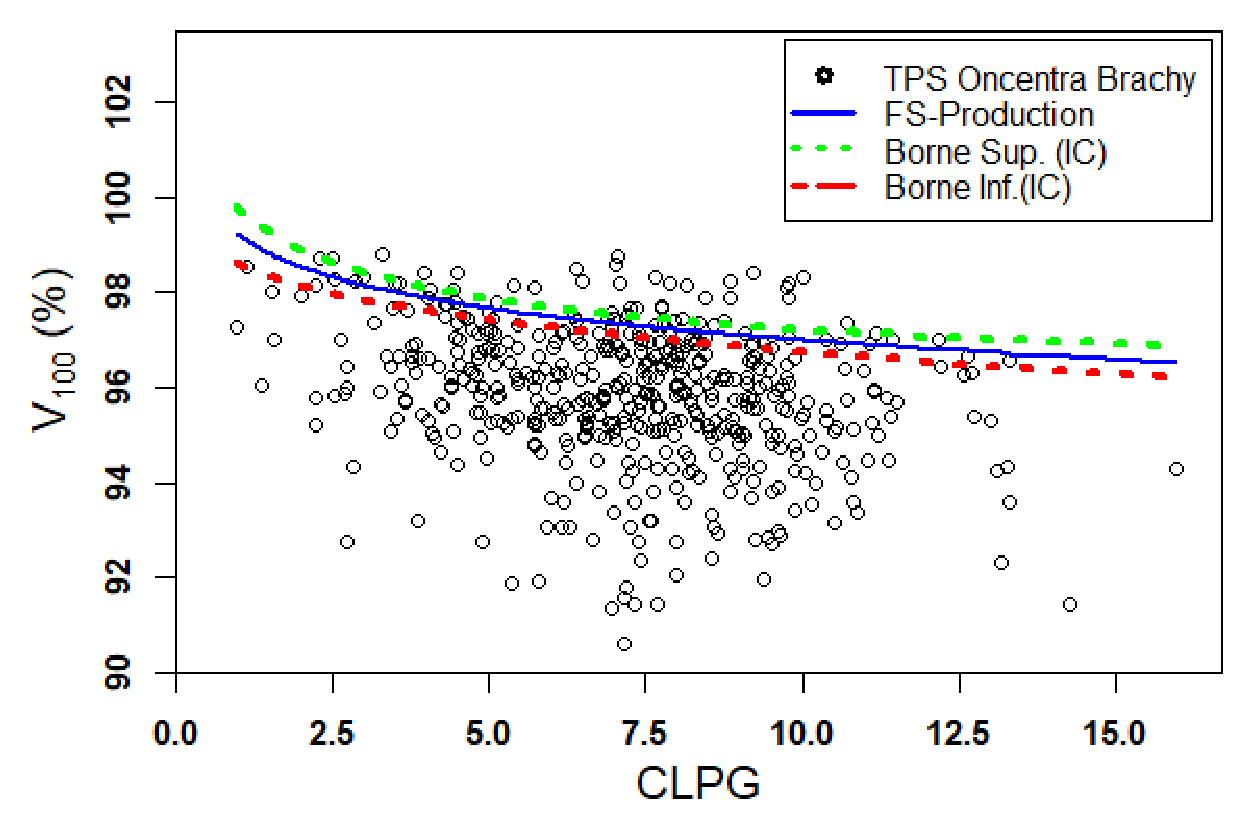
\includegraphics[width=7.2cm,height=5.2cm]{ModeleGlobalV100}\label{fig:ModeleGlobalV100}}
  \hspace{0.5cm}
  \subfloat{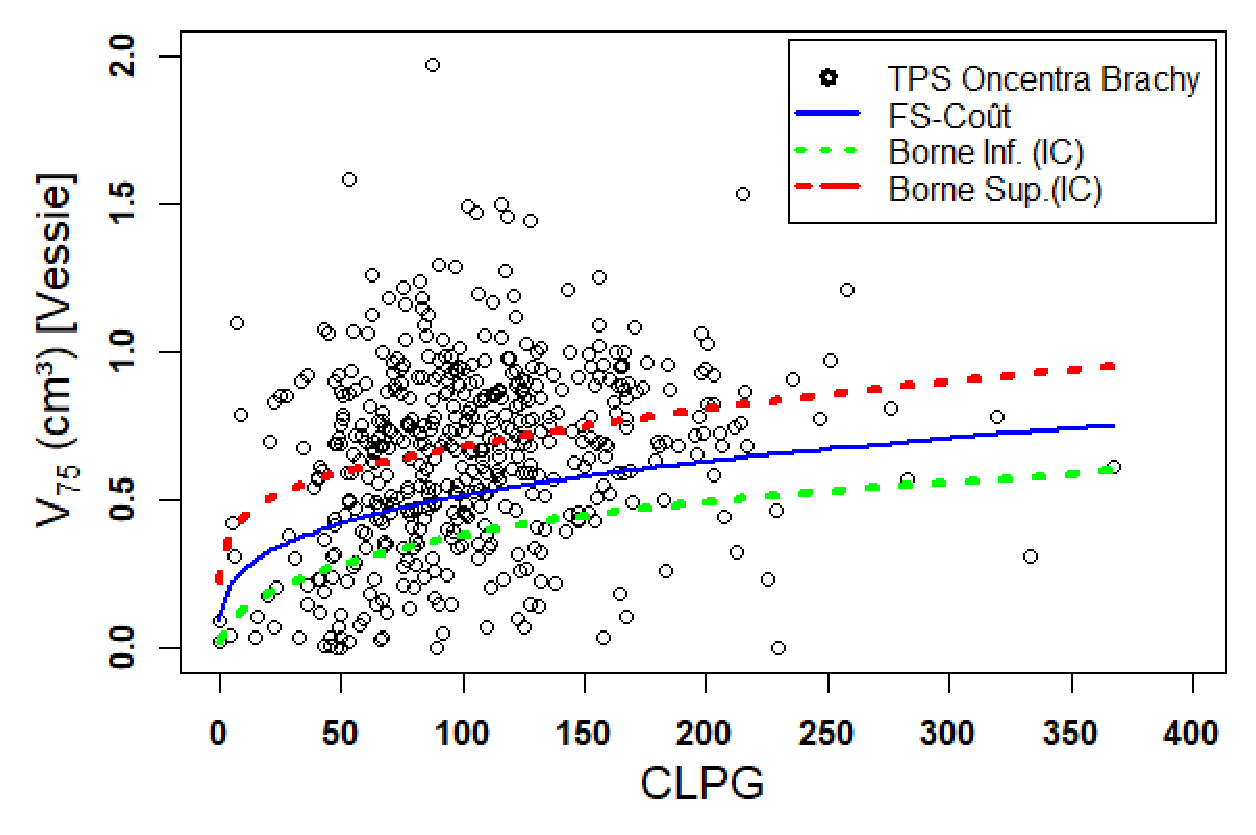
\includegraphics[width=7.2cm,height=5.2cm]{ModeleGlobalV75V}\label{fig:ModeleGlobalV75V}}
  \hspace{0.5cm}
  \subfloat{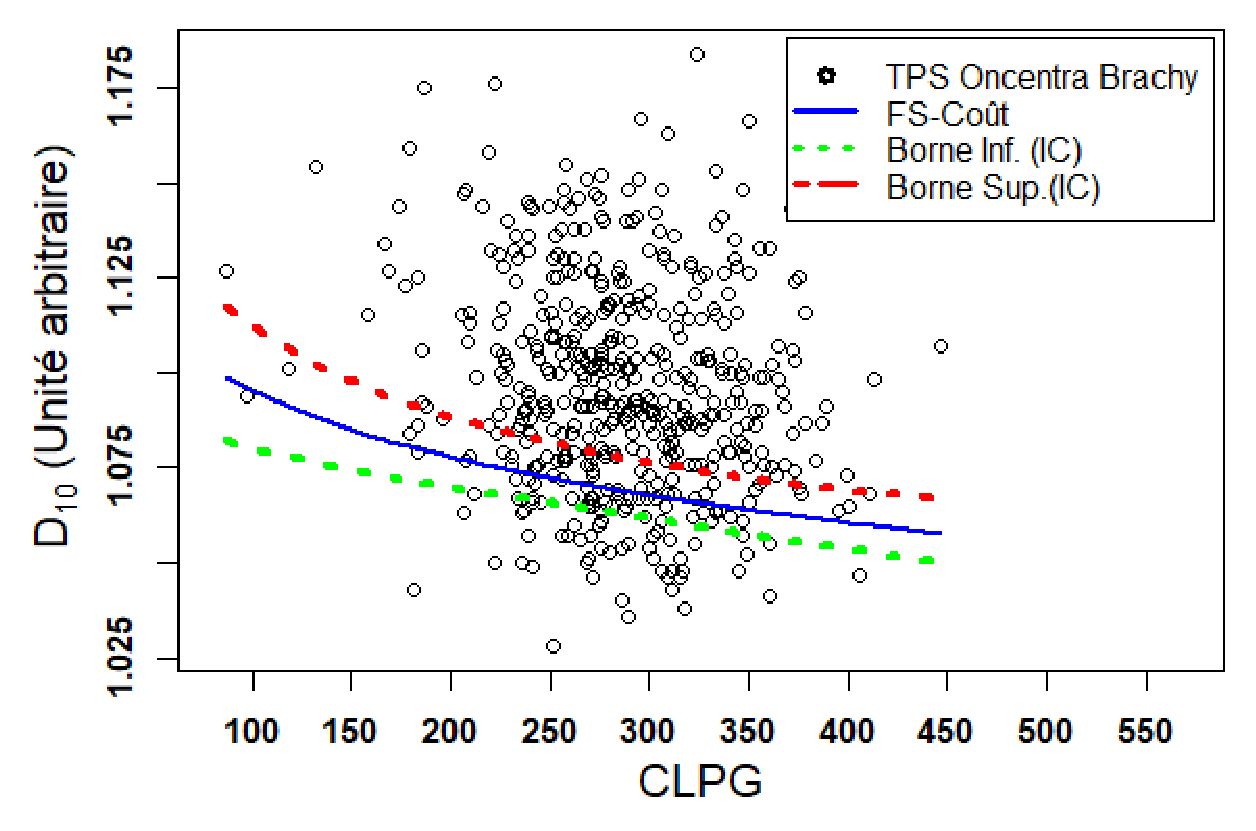
\includegraphics[width=7.2cm,height=5.2cm]{ModeleGlobalD10}\label{fig:ModeleGlobalD10}}
  \hspace{0.5cm}
  \subfloat{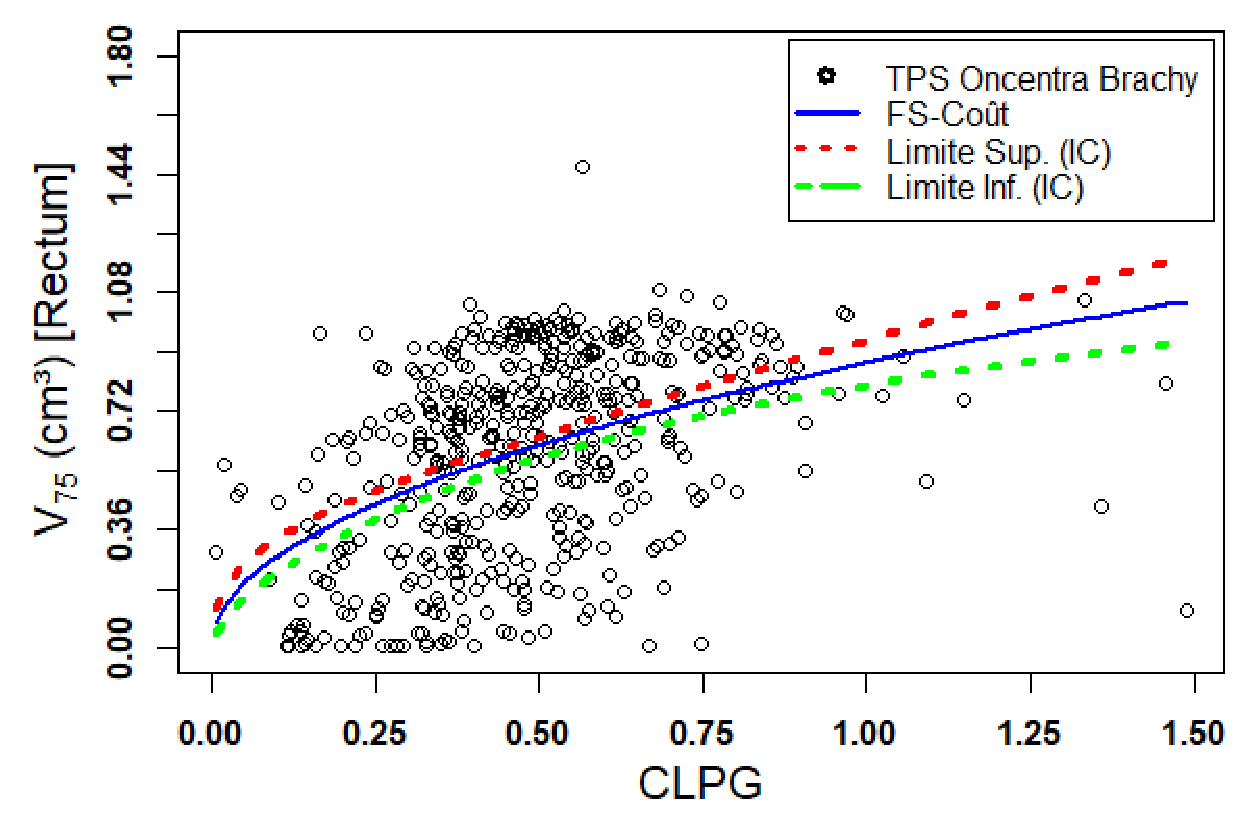
\includegraphics[width=7.2cm,height=5.2cm]{ModeleGlobalV75R}\label{fig:ModeleGlobalV75R}}
\caption{\label{ModelGlobalFS} Modèles de FS complets optimisés pour la couverture du CTV et la limitation de la dose aux OARs (vessie, rectum, urètres). CLPG est la combinaison linéaire des paramètres géométrique qui caractérise chaque plan (voir équation \ref{eqn:CLPG}.}
\end{figure}
%
Le croisement de l'ensemble de l’échantillon pour les trois modèles montre que le nombre de plans qui tombent simultanément dans les régions de confiance est de 3\%, c’est-à-dire, simultanément au-dessus de la frontière V$_{100}$ et en dessous des deux frontières V$_{75}$ (vessie) et D$_{10}$. Ce résultat témoigne le compromis auquel le planificateur est contraint de réaliser, entre la couverture maximale du CTV et la minimisation de la dose aux OARs. Cependant, le planificateur ne dispose d’aucun outil objectif lui permettant de juger sur la pertinence du compromis réalisé. Les présents modèles constituent un outil objectif et robuste pour uniformiser un tel compromis. En effet, un plan pour être considéré comme optimal du point de vue des présents modèles, doit se situer au moins sur chacune des frontières, c’est-à-dire, sur la frontière de V$_{100}$, V$_{75}$ et D$_{10}$; ceci amène à définir deux autres classes de plans, à savoir, les plans fortement optimisés pour la couverture du CTV, mais moins optimisés pour les OARs, inversement. Bien que ces plans restent cliniquement acceptables, le meilleur compromis pourrait correspondre à une situation d’équilibre pour laquelle, on diminue la couverture du CTV, ce qui va favoriser la minimisation de la dose aux OARs, tout en maintenant ledit plan sur ou au voisinage des trois frontières, inversement; 17\% des plans dans l’échantillon peuvent bénéficier d’un tel traitement tout en répondant aux objectifs cliniques.
%
\section{Analyse de l'échantillon test} \label{subsec:Echantest}
Les modèles ont été confrontés à un échantillon test constitué de 100 plans, afin d’évaluer leur capacité à détecter les plans améliorables, plans qui ne font pas partie de l’échantillon ayant servi à la construction des modèles, et par conséquent, mettre en évidence leur pouvoir prédictif. Les résultats quantitatifs détaillés sont présentés dans le chapitre 3 (section \enquote{Testing results}) qui est un projet d’article en voie de soumission. De façon succincte,  il en ressort qu’aucun plan n’a été identifié simultanément dans les régions de confiance des trois modèles. Ces modèles ont également identifié la proportion des plans qui sont améliorables du point de vue de la couverture du CTV et la minimisation de la dose aux OARs, et surtout, la proportion des plans qui peuvent bénéficier d’une augmentation de la couverture du CTV (V$_{100}$) au prix d’une augmentation de la dose aux OARs, mais en maintenant ces derniers en dessous de leurs frontières V$_{75}$ et D$_{10}$. Le pouvoir prédictif des modèles a donc été mis en évidence, ainsi qu’une limitation importante de ces derniers. En effet, le pouvoir prédictif des modèles n’est valable que dans le domaine du profil de paramètres géométriques de l’échantillon sur lequel les modèles sont construits; une proportion de cet échantillon test n’est donc pas incluse dans cette analyse, suite à cette limitation, laquelle peut être améliorée en élargissant la taille de l'échantillon sur lequel les modèles ont été optimisés. 
%
\section{Développements futurs et validation clinique} \label{developementsfuturs}
\subsection{Paramètres géométriques}
Le profil de paramètres géométriques est une donnée importante sur laquelle repose la précision des modèles. Les paramètres géométriques retenus dans ce projet ne sont certainement pas les plus exhaustifs que l’on pourrait imaginer; on pourrait élargir ceux-ci en tenant compte par exemple du gradient d’expansion du volume des OARs (vessie, rectum). En effet, en curiethérapie, les volumes contourés des OARs (vessie, rectum) ne chevauchent pas avec la prostate, mais la mesure de la vitesse avec laquelle un chevauchement aurait lieu (gradient de chevauchement) si une expansion homogène autour de la vessie et le rectum était réalisée pourrait avoir un impact sur la précision des modèles. D’autre part, la distance de Hausdorff prise en compte dans le registre des paramètres géométriques dans cette étude est la distance maximale; on pourrait tester l’impact sur les modèles avec la distance minimale, ou moyenne.
%
\subsection{Ordre des paramètres géométrique}
L’impact de chaque paramètre géométrique du modèle à $n$ paramètres par rapport au modèle à $n-1$ paramètres a été évalué par le biais du calcul de la p-value, mais dans un ordre bien déterminé (voir la section \ref{subsec:Comb.Lineaire}). Une étude sur les différentes permutations possibles en gardant le volume du CTV comme modèle de base, pourrait révéler des informations exploitables dans le sens de l’amélioration des modèles. Cependant, une telle étude va nécessiter une puissance de calcul, car pour le modèle de CTV à 8 paramètres géométriques, cela représente 5040 frontières à optimiser, le modèle de base restant fixe (volume du CTV). 
%
\subsection{\texorpdfstring{Hypothèse de normalité} {Hypothèse de normalité sur u}}
Les résultats présentés dans ce projet reposent sur plusieurs hypothèses dont l’impact sur la précision des modèles mérite d’être évalué. En effet, les modèles sont construits sur l’hypothèse de normalité sur la composante de la variable aléatoire $\epsilon$ qui mesure l’efficience technique, c’est-à-dire, $u$ est distribuée selon une loi normale tronquée positive, $N^{+}(0, \sigma^{2}_{u})$. Bien que cette hypothèse soit largement la plus utilisée dans la littérature, il convient de souligner que d’autres distributions pourraient être testées afin d’évaluer la précision des modèles avec le choix de la distribution de $u$, exemple d’une distribution normale tronquée positive de mode $\mu$ \cite{Stevenson@1980}, ou d'une distribution Gamma \cite{ Greene@1990}. 
%
\subsection{Validation clinique}
Les modèles finaux après un éventuel réajustement au niveau des paramètres géométriques, se doivent d’être validés cliniquement. Cette validation peut se faire de deux façons: (1) replanifier les plans de l’échantillon test qui ont été identifiés comme améliorables (section \ref{subsec:Echantest}), ou (2) confronter les modèles lors de la planification des nouveaux patients. Quel que soit le cas de figure, une analyse doit être faite afin d’évaluer le degré par lequel les valeurs prédites par les modèles sont atteintes ou approchées, et procéder à des ajustements au besoin.
%             % chapitre 1
\chapter{A stochastic frontier analysis for enhanced treatment quality of High-Dose-Rate brachytherapy plans} % numéroté
%
\section{Résumé} 
%
\section{Abstract} 
\noindent The purpose of the present study is to develop a quality control (QC) model based on patient-specific geometric parameters, using the stochastic frontier analysis, a method of economic modeling. The built models act as QC tool by predicting in advance (before the treatment process starts) the final dosimetry achievable for an HDR brachytherapy prostate plan. Geometric parameters involved in the modelling process are the contoured volumes (CTV, OARs), the Hausdorff distance between CTV and OARs, and a third parameter measuring the degree of non-parallelism of catheters within the target volume. Dosimetry parameters of interest are V$_{100}$ for the CTV, V$_{75}$ (bladder, rectum) and D$_{10}$ (urethra). Results show that the built models can provide valuable information on the personalization of the optimization process based on the patient geometric parameters. The impact on the quality plan due to the planner's experience variability and judgment is reduced by using these models. Furthermore, a good trade-off between the target volume coverage and OARs sparing does not longer depend on the planner's judgment, but can be achieved by moving each plan at least around their respective frontier for V$_{100}$, V$_{75}$ and D$_{10}$. The use of these models can be extended as a robust benchmarking tool for comparison of plans quality obtained from different optimization techniques, as well as, among different institutions, and for selecting optimized plans for a knowledge-based study. The overall results demonstrate that optimized plans from a TPS, even clinically acceptable, are not necessarily the best that can be achieved.\newline
\newline
\textbf{Keywords} Stochastic frontiers analysis, brachytherapy, geometric parameters, quality control, confidence intervals.\newline
%
\section{INTRODUCTION}
\lettrine[nindent=0em,lines=2]{T}{}he goal of radiotherapy is to deliver a prescribed dose to the target volume, consistent  with  maintaining  complication  rates to surrounding tissues and organs at risk (OAR) within an  
acceptable level. This can be acheived by using brachytherapy technique, the most conformal radiation therapy used to tread several kinds of cancer such as, prostate, breast and cervical. Depending of the lesions involved in the treatment process, this radiation therapy modality can be performed in many ways known as, Intra-cavity Brachytherapy, Intertitial Brachytherapy, Intraluminal Brachytherapy and surface applications \cite{podgorsak@2005, khan@2014}. High Dose Rate (HDR) brachytherapy modality use small radioactive sealed source such as Iridium-192 which is automatically handled from a remote afterloading unit. This source allows a high dose rate and the superior dose distribution in the target volume, while lowering radiation exposure to the workers in an acceptable level. However, the ability to meet clinical objectives during a treatment planning process depends on several factors, such as the accuracy of dose calculation algorithm, the optimization method used to compute dwell times at dwell positions of the radioactive source along specified applicator paths, as well as the planer’s experience variability and judgment. Most optimization methods focus on obtaining desired doses at a number of predefined points by the planner, and the treatment planning process is stopped when computed dwell time matches as closely as possible the desired doses constraints at these selected points. Besides, at the starting point of a treatment planning process, information about the maximum  clinical target volume (CTV) coverage, the trade-off between OAR sparing and CTV dose homogeneity are usually unknown in advance. In forward optimization scheme, the planner is often required to adjust manually and iteratively dwell times and weights and compares the resulting dose distribution to the clinical objectives. In an inverse optimization scheme, case of Inverse Planning by Simulated Annealing (IPSA) \cite{lessard@2001, lessard@2002,Lessard2004}, the user manually modifies the weighing factor value of the cost function until dose objectives defined for each organ are fulfilled or when the cost function has reached its global minimum value.  As a consequence, a strong interaction between the planner and the Treatment Planing System (TPS) is an important step in producing an optimized plan. Moreover, criteria of CTV coverage, as well as the dose limit to OAR guiding the treatment planning process are usually those recommended by international organizations such as the American Brachytherapy Society (ABS) \cite{ABS} or task group such as the Radiation Therapy Oncology Group. RTOG 0924 \cite{RTOG}. Since these recommendations are based on randomized clinical trials, they do not, therefore, account for patient-to-patient variability of geometric parameters which play an important role on the balance between the CTV coverage and OAR sparing. Thus, whatever the optimization method used, even though a treatment plan is consistent with clinical objectives, it is therefore possible that the latter is not the most optimal that can be achieved based on the geometric parameters of the treatment plan concerned. \newline
The original contribution of this paper is the introduction of a new concept of quality control for HDR brachytherapy plans, using stochastic frontier analysis, a method of economic modeling. The models will act as a quality control tool of treatment plans, by predicting dosimetric parameters values attainable at the starting point of the treatment planning process. These models will provide valuable indications in advance, on the level of dose reduction to OARs, as well as, the target volume coverage achievable. It is therefore expected that the plan quality will be lesser dependent of the optimization method used, the planner's experience variability and judgment. Furthermore, the planner's treatment time will be effectively managed since the planning process could be stopped at the right time.
%
\section{MATERIALS AND METHODS}
%
\subsection{Stochastic frontier analysis}
%
\subsection{Patients geometric parameters}
%
\subsection{Optimization process and models accuracy}
%
\section{RESULTS}
\subsection{Goemetric parameters selection}
%
\subsection{Modeling results}
%
\subsection{Testing results}
%
\section{DISCUSSION}
%
\section{CONCLUSION}
%
\section{Acknowledgments}
This work was partly supported by the CREATE Medical Physics Research Training Network grant of the Natural Sciences and Engineering Research Council (Grant number: 432290) and the Fellowships Program of the \enquote{Ministère de la Santé et des Services sociaux}. The authors are greatly indebted to the radiation oncology physicists Ms. Marie-Claude Lavallée and Annie Letourneau, medical physicists at the Hôtel-Dieu de Québec (Québec, Canada), for their help in  collecting patient sample for the development of this project. 

    % chapitre 3, etc.

\chapter{Conclusion}         % ne pas numéroter
%\phantomsection\addcontentsline{toc}{chapter}{Conclusion et développements futurs} % dans TdM
% * <larchamb@gmail.com> 2017-08-30T18:34:15.098Z:
% 
% > \chapter*{Conclusion et développements futurs}         % ne pas numéroter
% Voir commentaire de l'introduction: je préfère que ces sections soient numérotés
% 
% ^ <larchamb@gmail.com> 2017-08-30T18:34:49.476Z.
\lettrine[nindent=0em,lines=2]{L}{}a radiothérapie fait partie des différentes techniques principales de lutte contre le cancer, d’où sa parfaite intégration dans les différentes stratégies de traitement multidisciplinaires actuelles. Il s’agit d’une discipline qui est en constante évolution, bénéficient ainsi de nouveaux développements sur le plan de l’imagerie, de l’informatique, ainsi que des équipements de traitement. Particulièrement en curiethérapie, l’arrivée de l’imagerie échographique transrectale pour l’implantation des cathéters dans les volumes cibles fût une étape déterminante pour faire entrer la curiethérapie dans le $21^{\grave{e}me}$ siècle, suivie de l’arrivée des projecteurs de sources (curiethérapie HDD et débit de dose pulsé), et le développement de nouveaux algorithmes d’optimisation de dose. Ces mutations ont contribué à améliorer la prise en charge des patients dans l’atteinte des objectifs cliniques, mais ont aussi complexifié les pratiques, ce qui justifie l’évolution des méthodes contrôle de qualité permettant de garantir avec un niveau de confiance suffisant la cohérence d’une prescription médicale et l’exécution sécuritaire de celle-ci, afin de délivrer la dose prescrite au volume cible, tout en minimisant la dose aux tissus normaux alentour. Malgré ces évolutions remarquables, la qualité du plan qui résulte de la phase d’optimisation de la dose reste toujours tributaire de l’expérience et le jugement du planificateur. En effet, un plan pour être jugé cliniquement acceptable, doit respecter les recommandations sur la couverture du CTV (V$_{100}$ > 90\%) et les limites de dose aux OARs, à savoir, V$_{75}$ < 1 cm$^{3}$ (vessie, rectum) et (V$_{125}$ < 1 cm$^{3}$, D$_{10}$ < 118\% de la dose de prescription) pour l’urètre. On pourrait cependant se poser la question si un plan jugé clinique est forcément optimal. À partir de quel point un plan peut-il être jugé optimal dès lors qu’il est clinique? Le planificateur ne dispose d’aucun outil objectif lui permettant de répondre à cette question, il décide donc sur le caractère optimal d’un plan sur la base de son expérience et son jugement, d’où l’intérêt de ce projet; développer les modèles de frontière stochastique pour l’amélioration de la qualité des plans en curiethérapie haut débit de dose pour le cancer de la prostate. L’analyse de frontière stochastique qui est l’outil sur lequel repose le présent projet est un formalisme dont la paternité revient aux économistes. Lesdits modèles devront guider le processus de planification en prédisant, sur la base du profil de paramètres géométriques spécifiques à chaque patient, les paramètres dosimétriques qui caractérisent la couverture du CTV, ainsi que la minimisation de la dose aux OARs. Il sera donc possible grâce à ces modèles de minimiser l’impact du jugement et l’expérience propre à chaque planificateur sur la qualité du plan final. Quatre modèles ont été construits sur les paramètres dosimétriques qui présentent une variabilité inter-patient, sur la base d’un échantillon de 495 plans des patients traités en une fraction de 15 Gy sous images CT (complément de la radiothérapie externe).
Les résultats des modèles optimisés sur la base de cet échantillon montrent que ceux constituent un outil fiable pour la prédiction des paramètres dosimétriques pour le CTV, la vessie et l’urètre. Les modèles ont permis de montrer la variabilité de la qualité des plans finaux pour des patients ayant un profil de paramètres géométriques semblables. Cette variabilité est plus importante pour la couverture du CTV que pour la limitation de la dose aux OARs (vessie, urètre). Cette grande variabilité témoigne la signature du jugement et l’expérience inhérente à chaque planificateur, sur la qualité du plan final. Les présents modèles peuvent aider à minimiser cet effet, puisque ceux fournissent des informations sur la dosimétrie atteignable sur chaque patient; ce qui va motiver le planificateur à poursuivre le processus d’optimisation, afin d’obtenir ou d'approcher les indices dosimétriques prédits par les modèles, ou inversement, c’est-à-dire, arrêter le processus d’optimiser au bon moment (gestion efficace du temps). Le caractère subjectif sur le concept du meilleur compris peut également être limité grâce aux présents modèles, le meilleur compromis correspondant au cas pour lequel, chaque plan se trouverait ou serait proche des frontières des différents modèles. Le modèle optimisé pour le rectum ne contient aucune information prédictive puisque la composante de l’efficience technique est nulle. Ceci s’explique par le fait que les physiciens, sous recommandation des radio-oncologues s’évertuent beaucoup dans l’optimisation de cet organe, parfois au détriment de la vessie, ceci justifie également la faible variabilité inter-planificateur pour l’optimisation de cet organe, en comparaison avec la couverture de CTV. Outre l’information prédiction contenue dans les modèles, ceux-ci peuvent servir pour d’autres applications, par exemple, ils constituent un outil robuste dans la sélection de meilleurs plans dans un échantillon existant. \\
En conclusion, les résultats du présent projet constituent une avancée dans la démarche visant à développer des modèles plus complets et cliniquement fiables. En effet, les modèles développés doivent passer par une phase de test clinique. D’autre part, ils pourraient aussi être améliorés si les différents points soulevés dans la section (\ref{developementsfuturs}) du chapitre \ref{chapitre2} sont étudiés et intégrés dans le processus d’optimisation de ces derniers. En fin, les résultats présentés dans ce travail reposent sur un échantillon de patients sous images CT, la question quant à leurs validités sous images échographiques mérite une investigation.             % conclusion

\appendix                       % annexes le cas échéant

%\chapter{Titre de l'annexe}     % numérotée
Texte                % annexe A
\bibliographystyle{IEEEtran} 
\bibliography{references} 
%\bibliography{IEEEabrv, references} % mon fichier de base de données s'appelle references.bib
%
\end{document}
